%\documentclass[b5paper,final,11pt,fleqn,twoside]{book}

\documentclass[a4paper,twoside,12pt]{report}
\usepackage{times}
\usepackage{graphics}

\usepackage{weso}

%
% cabeceras.tex
%
% Copyright 2003, Diego Berrueta Muñoz
%
% Cabeceras comunes
%

\usepackage[T1]{fontenc}

%Glosario

\usepackage[toc,style=treenoname,order=word,counter=section]{glossaries}

\usepackage{xspace}


\usepackage{tikz,times}
\usetikzlibrary{mindmap,backgrounds}

% cambia algunas fuentes (utilidad dudosa)
\usepackage[scaled=0.92]{helvet}
\usepackage{pifont}
\usepackage{courier}

% cambia algunas fuentes en modo matemático a Palatino
\usepackage{mathpazo}

% españolización
\usepackage[spanish]{babel}
\usepackage[utf8]{inputenc}
%\extrasspanish

% gráficos y colores
\usepackage{rotating}
\usepackage{graphicx}
\usepackage{color}
%\usepackage[all]{xy}
%\usepackage{pstricks}
\usepackage{pst-node}
%\usepackage[dvips,usenames]{pstcol}
%\usepackage{pdftricks}
%\usepackage{pst-uml}  % para hacer diagramas UML
%\usepackage{rail}     % para hacer diagramas de gramáticas

% mejoras visuales
\usepackage{enumerate}
\usepackage{fancyhdr}  % para configurar los encabezados
\usepackage{fancybox}  % para hacer cajitas
\usepackage[normal,oneline,sf,bf]{caption2}
\usepackage{titlesec}  % para configurar los títulos de sección
\usepackage{paralist}


\usepackage{epigraph}

% citas, referencias e índices
\usepackage{cite}
%\usepackage{citesort}   % da errores al compilar
\usepackage{makeidx}

% incrustaciones de código fuente
%\usepackage[norules,nolineno]{lgrind}
\usepackage{verbatim}
\usepackage{listings}
%\usepackage{noweb,a4wide}


%\usepackage{textcomp}
\usepackage[right]{eurosym}

% columnas
\usepackage{multicol}

% tablas
\usepackage{longtable}
%\usepackage{ltxtable}

% impresión elegante de URLs
\usepackage{url}

\makeatletter
\def\url@pfcstyle{%
  \@ifundefined{selectfont}{\def\UrlFont{\sf}}{\def\UrlFont{\small\ttfamily}}}
\makeatother
%% Now actually use the newly defined style.
\urlstyle{pfc}


% márgenes
\usepackage[a4paper, left=30mm, right=20mm, top=25mm, bottom=25mm]{geometry}
%\usepackage[a4paper, left=20mm, right=20mm, top=25mm, bottom=25mm]{geometry}

% 
% \usepackage[a4,center,cam]{crop}
\usepackage{blindtext}

% salida en PDF navegable
%\usepackage{hyperref}
\usepackage[plainpages=false,colorlinks, linkcolor=black]{hyperref}

% quitar en versión final
%\usepackage{showkeys}   % depuración de etiquetas y referencias
%\usepackage{showidx}    % depuración de índice

% configuración del paquete "listings"

\lstset{%
        %language=Java,
	basicstyle=\footnotesize\sffamily,
	keywordstyle=\bfseries, %\color{darkred}
 	stringstyle=\itshape, %\color{violet}
 	commentstyle=\itshape, %\color{blue}
 	showspaces=false,
 	showtabs=false,
 	showstringspaces=false,
 	frame=trBL,
        frameround=tttt,
        %backgroundcolor=\color{lightyellow},
	inputencoding=utf8,
 	extendedchars=true,
 	numbers=none,
        aboveskip=0.5cm,
        belowskip=0.5cm,
        xleftmargin=1cm,
        xrightmargin=1cm,
	breaklines=true
}
\definecolor{darkred}{rgb}{0.5, 0, 0}
\definecolor{violet}{rgb}{1, 0, 1}
\definecolor{lightyellow}{rgb}{1,1,0.8}


%%%%%%%%%%%%%%%%%%%%%%%%%%%%%%%%%%%%%%%%%%%%%%%%%%%%%%%%%%%%%%%%%%%%%%
% cabeceras y pies de página (con el paquete "fancyhdr")
\headheight 15pt
%\addtolength{\headwidth}{\marginparsep}
%\addtolength{\headwidth}{\marginparwidth}
%\renewcommand{\chaptermark}[1]{\markboth{\MakeUppercase{#1}}{}}
%\renewcommand{\sectionmark}[1]{\markright{\thesection\ #1}}
%\fancyhead[LE,RO]{\textbf{\thepage}}
%\fancyhead[RE]{\textit{\leftmark}}
%\fancyhead[LO]{\rightmark}
%\fancyfoot[LCR]{}
\fancyhead{} % Todos los campos en blanco en la cabecera
\fancyfoot{} % Lo mismo al pie
\fancyhead[RO, LE]{\thepage}
\fancyhead[LO, RE]{\slshape\leftmark}
\renewcommand{\headrulewidth}{0.5pt}
\renewcommand{\footrulewidth}{0.5pt}


%%%%%%%%%%%%%%%%%%%%%%%%%%%%%%%%%%%%%%%%%%%%%%%%%%%%%%%%%%%%%%%%%%%%%%
% títulos de secciones (con el paquete "titlesec")
\titleformat{\chapter}[display]
	{\fontfamily{pag}\selectfont\Huge}
	{\LARGE\chaptertitlename\ \thechapter}{20pt}{\bfseries}
\titleformat{\section}
	{\fontfamily{phv}\selectfont\LARGE}
	{\thesection}{1em}{\bfseries}[\titlerule]
\titleformat{\subsection}
	{\fontfamily{phv}\selectfont\Large}
	{\thesubsection}{1em}{\bfseries}
\titleformat{\subsubsection}
	{\fontfamily{phv}\selectfont\large}
	{\thesubsubsection}{1em}{\bfseries}


%%%%%%%%%%%%%%%%%%%%%%%%%%%%%%%%%%%%%%%%%%%%%%%%%%%%%%%%%%%%%%%%%%%%%%
% espaciado entre párrafos
\addtolength{\parskip}{+0.2cm}


%%%%%%%%%%%%%%%%%%%%%%%%%%%%%%%%%%%%%%%%%%%%%%%%%%%%%%%%%%%%%%%%%%%%%%
% salida en PDF navegable (con el paquete "hyperref")
\hypersetup{bookmarks,
	bookmarksnumbered,
%	colorlinks, % quitar en las versiones impresas
	hyperindex,
	%linkcolor=red,
	%anchorcolor=black,
	%citecolor=green,
	citecolor=violet,
	%filecolor=magenta,
	%menucolor=red,
	%pagecolor=red,
	%urlcolor=cyan,
	pdftitle={PhD. Dissertation-Jose María Alvarez Rodríguez},
	pdfauthor={Jose María Alvarez Rodríguez}
	pdffitwindow,
	plainpages=false,
	pageanchor=false,
	pdfstartview={}}


%%%%%%%%%%%%%%%%%%%%%%%%%%%%%%%%%%%%%%%%%%%%%%%%%%%%%%%%%%%%%%%%%%%%%%
% profundidad de secciones y numeración
%\setcounter{tocdepth}{4}
\setcounter{secnumdepth}{3}


%%%%%%%%%%%%%%%%%%%%%%%%%%%%%%%%%%%%%%%%%%%%%%%%%%%%%%%%%%%%%%%%%%%%%%
% división silábica
\hyphenation{pu-bli-ca-ción con-tex-tua-li-za-ción pro-ble-mas Mi-nis-te-rio li-ci-ta-ción si-guien-tes desa-rro-llar con-tra-ta-ción pan-europea fa-ci-li-tar in-ter-opera-bility
 elec-tró-ni-ca li-ci-ta-do-ras he-te-ro-gé-neos res-trin-gi-do cons-cien-te de-sa-rro-lla-da mo-de-lo paí-ses ge-ne-ra-da
 par-ti-ci-pa-ción ad-mi-nis-tra-ti-vos bi-blio-gra-fía re-gis-tra-do-ra ad-mi-nis-tra-ti-va ca-rac-te-rís-ti-cas
 Pa-ra-le-la-men-te des-cri-ben vo-ca-bu-la-rio me-dian-te do-cu-men-to di-fe-ren-tes bi-blio-gra-fía mo-de-lo
 ve-ri-fi-ca rea-li-zar res-tric-ciones Por ejem-plo su-ge-ren-cias mo-de-los rea-li-za si-guien-do he-te-ro-gé-neas ello
 ra-zo-na-ble li-mi-ta-cio-nes reu-ti-li-cen ini-cia-ti-va va-ria-da exis-ten ob-te-ner con-ti-nua-men-te me-dian-te ins-ti-tu-ción
 pro-pues-ta pu-bli-ca-ción ca-tá-lo-go mo-ni-to-ri-za-ción vi-sua-li-za-ción mo-de-los co-rres-pon-dien-tes
 re-fe-ren-cia re-la-ti-vas par-ti-cu-lar  ele-men-to mo-de-la-do se-le-ccio-na-do pro-du-cción Re-con-ci-lia-ción des-crip-cio-nes broader-Transitive 
 de-pen-dien-do Ca-tá-lo-gos vo-ca-bu-la-rios Pro-pie-ta-rio des-plie-gue De-sa-rro-lla-dor mo-de-lar res-pues-ta si-mi-la-res rea-li-za-do SE-RI-MI 
Evol-ving ha-bi-li-tar rea-li-za-ción pu-bli-ca-ción ge-ne-ra-ción rea-li-za-ban ac-tua-li-za-ción ac-ce-so ha-cer es-tán-dar 
vo-ca-bu-la-ry con-si-de-ra-do des-cri-bir pu-bli-car pu-bli-ca-dos ta-xo-nó-mi-ca Pro-duct-on-to-lo-gy Va-lo-res in-terope-ra-bi-li-dad MOL-DEAS 
man-te-ni-mien-to re-pre-sen-tar ta-xo-no-mías des-crip-ción ge-ne-ra cons-truc-ción re-pre-sen-tan-do rea-li-za-das trans-fe-ren-cia 
uti-li-za-ble pu-bli-ca be-ne-fi-cios res-pon-sa-bi-li-da-des rea-li-zan Ad-mi-nis-tra-ción con-ti-nua-ción prio-ri-ta-rio ICT 
in-terope-ra-ble ge-ne-ra-do con-fi-gu-ra-cio-nes rea-li-zan-do rea-lis-ta má-xi-mo Cons-ti-tu-yen-do pro-ble-ma po-si-bi-li-dad ma-yor coo-pe-ra-ción 
ra-zo-na-mien-to Des-crip-tion con-cep-tua-li-za-ción de-sa-rro-lla-dos ope-ra-do-res axio-mas go-bier-no or-ga-nis-mos éxi-to 
si-guien-te do-mi-nios pro-duc-ción Na-tio-nal orien-ta-da ló-gi-ca in-di-vi-duos di-se-ña-do for-ma-li-za-dos ta-xo-no-mía 
auto-má-ti-ca ca-li-dad re-co-men-da-ble ad-mi-nis-tra-ti-vo su-mi-nis-tre error ca-rac-te-rís-ti-ca ele-men-tos he-rra-mien-tas 
eva-lua-ción res-pec-to Ad-mi-nis-tra-cio-nes ex-pe-ri-men-tal orien-ta-das re-gis-tros do-cu-men-tos má-xi-ma je-rar-quía 
sa-tis-fac-to-rios obs-tan-te con-su-mi-dos con-fe-ren-cias SPARQL rea-li-za-dos va-lo-ran eco-no-mi-zar fle-xi-ble ex-pe-dien-te 
pro-ce-di-mien-to usan-do ame-ri-ca-nas fa-mi-lia ni-vel ra-zo-na-do-res re-pre-sen-ta-ción lo-ca-li-za-do Man-ches-ter 
en-ri-que-ci-mien-to he-rra-mien-ta rea-li-zar-se prio-ri-ta-rios Li-ci-ta-cio-nes ne-ce-sa-rios ma-te-ria-li-zan es-pe-cia-li-zán-do-se 
Com-pu-ting pla-ni-fi-ca-ción cua-li-ta-ti-va de-sa-for-tu-na-da-men-te li-de-ra-do ma-te-ria-li-za-do Cons-tructs 
ma-te-ria-li-za WESO en-ten-di-mien-to MOLDEAS ela-bo-ra-ción re-fe-ren-te re-gis-tra-tion uni-la-te-ral po-si-bi-li-tar ope-rar 
in-ter-ope-ra-bles ad-mi-nis-tra-ti-vas fle-xi-bi-li-dad auto-no-mía co-mer-cio procesa-miento de-sa-rro-llan-do meta-in-for-ma-ción 
apro-pia-dos li-mi-ta-do es-pe-cia-li-za-ción ló-gi-cas in-de-pen-dien-te-men-te ge-ne-ral dis-po-ner dis-mi-nu-yen-do co-rrien-te 
rea-pro-ve-char de-sa-rro-llo ge-ne-ral Ins-ti-tu-te com-pu-ting pos-te-rior con-su-mi-da mi-llo-nes Fi-gu-ras cons-tan-te equi-va-len-cia ope-ra-cio-nes 
fac-to-ri-za-ción Res-pon-sa-bles Geo-Linked-Data reu-ti-li-za-ción co-rrec-tos trans-for-ma-ción bien con-si-guien-te des-cu-brien-do 
geo-rre-fe-ren-cia-ción pro-li-fe-ra-ción cum-pli-mien-to Ne-go-tia-ted uti-li-dad ma-nual es-pe-cia-li-za-ción ma-yo-ría mo-de-la 
des-cu-bri-mien-to rea-li-za-da pu-bli-can se-lec-cio-nar me-ca-nis-mos fun-cio-na-li-dad ve-ri-fi-car ines-pe-ra-dos re-gis-tro 
pro-pues-tos trans-pa-ren-te va-ria-bles bi-blio-te-ca bi-blio-te-cas adap-ta-bi-li-dad in-ter-co-ne-xión va-ria-ble vi-sua-li-zar 
ope-ra-ti-vo ge-ne-rar su-mi-nis-tra-dos va-li-da-ción su-mi-nis-tra-dores pro-pie-da-des hi-po-ni-mia re-cu-pe-ra-dos in-de-pen-dien-te-ment-te 
triun-fo reu-ti-li-za-ción ge-ne-ral apro-xi-ma-ción va-ria-bi-li-dad teó-ri-cas con-ti-nuo di-se-ño des-afor-tu-na-da-men-te In-dus-trial prin-ci-pios 
di-fe-ren-cia-das eva-lua-dos re-qui-si-tos co-la-bo-ra-cio-nes co-la-bo-ra-ción in-dus-tria-les Se-venth pon-de-ra-do re-po-si-to-rios 
ex-pe-ri-men-ta-les pu-bli-ci-tar co-la-bo-ra-ción bi-llo-nes Doc-to-ra-do re-so-lu-ción cul-tu-ra-les trans-cur-so Pa-rro-quias Lo-gics co-rrec-to 
sig-ni-fi-ca-do Aña-dien-do ope-ra-ción ma-ne-ra agi-li-zar con-fian-za per-so-na-les in-al-te-ra-dos re-la-ti-vos des-cri-bien-do 
se-ña-la-das vo-ca-bu-la-ries con-tex-tua-li-za-da Ba-rras cir-cuns-cri-bién-do-se for-ma-li-za-ción fa-ci-li-tan-do re-ali-men-ta-ción 
re-fe-ren-cias ma-ni-fes-tar-se CKAN lo-ca-li-dad dia-gra-ma ver-da-de-ra-men-te es-ta-ble-ci-mien-to con-si-de-ra ta-reas co-rrec-ta 
co-he-ren-te pos-te-rior-men-te apro-pia-das exac-tos va-rios pro-pues-to ex-pe-ri-men-to re-fe-ren-tes orien-ta-dos ha-bi-tual con-cre-tas 
con-fi-gu-ran afi-lia-ción Gi-ner va-lo-ra-ción res-pon-sa-bi-li-dad}   

%%Tablas
\addto\captionsspanish{
        \def\listtablename{\'Indice de tablas}%
        \def\tablename{Tabla}} 

%%%Math
\usepackage{latexsym}
\usepackage{amsmath}
\usepackage{amssymb}
\usepackage{amsthm}

\usepackage{algorithm}
\usepackage{algorithmic}
\usepackage{multirow}
\usepackage{rotating}


\newtheorem{theorem}{Theorem}[section]
\newtheorem{proposition}[theorem]{Proposición}
\newtheorem{lemma}[theorem]{Lema}
\newtheorem{definition}[theorem]{Definición}
\newtheorem{examples}[theorem]{Ejemplos}
\newtheorem{remarks}[theorem]{Remarks}
\newtheorem{corollary}[theorem]{Corolario}
\newtheorem{remark}[theorem]{Remark}
\newtheorem{example}[theorem]{Ejemplo}
\newtheorem{conjecture}[theorem]{Conjecture}
\newtheorem{note}[theorem]{Nota}



\newsavebox\FrameBox
\newenvironment{Frame}{%
  \par\setbox\FrameBox\hbox\bgroup\minipage{0.9\textwidth}\parskip\baselineskip\ignorespaces
}{%
  \endminipage\egroup\fbox{\box\FrameBox}\par
}

\newcommand{\si}{$\oplus$\xspace}
\newcommand{\no}{$\ominus$\xspace}
\newcommand{\na}{$\odot$\xspace}


%Extraer
\newcommand{\linkeddata}{\textit{Linked Data}\xspace}
\newcommand{\opendata}{\textit{Open Data}\xspace}
\newcommand{\lod}{\textit{Linking Open Data}\xspace}
\newcommand{\ogd}{\textit{Open Government Data}\xspace}
\newcommand{\datasets}{\textit{datasets}\xspace}
\newcommand{\dataset}{\textit{dataset}\xspace}
\newcommand{\provenance}{\textit{provenance}\xspace}
\newcommand{\trust}{\textit{trust}\xspace}
\newcommand{\egov}{\textit{e-government}\xspace}
\newcommand{\pusi}{\textit{Public Sector Information}\xspace}
\newcommand{\gd}{\textit{Government Data}\xspace}
\newcommand{\wod}{Web de Datos\xspace}
\newcommand{\wode}{\textit{Web of Data}\xspace}
\newcommand{\eproc}{\textit{\gls{e-Procurement}}\xspace}
\newcommand{\gld}{\textit{Government Linked Data}\xspace}


%
% utilidades.tex
%
% Copyright 2003, Diego Berrueta Muñoz
%
% Algunos comandos y entornos utilizados
%


%%%%%%%%%%%%%%%%%%%%%%%%%%%%%%%%%%%%%%%%%%%%%%%%%%%%%%%%%%%%%%%%%%%%%%
% Para llamadas de atención al margen

\reversemarginpar

\newcommand{\attention}{%
  \mbox{}\marginpar{\raggedleft \large\bfseries ! $\rightarrow$}%
}

\newcommand{\InlineFIXME}[1]{%
  {\bfseries\color{red} FIXME: #1}%
}

\newcommand{\FIXME}[1]{%
  \attention{}{\color{red}\bfseries #1}%
}


%%%%%%%%%%%%%%%%%%%%%%%%%%%%%%%%%%%%%%%%%%%%%%%%%%%%%%%%%%%%%%%%%%%%%%
% Comandos específicos de este proyecto

\newcommand{\FechaEntregaPFC}{2011}
\newcommand{\TituloPFC}{MÉTODOS SEMÁNTICOS DE REUTILIZACIÓN DE DATOS ABIERTOS ENLAZADOS EN LAS LICITACIONES PÚBLICAS}
\newcommand{\NumeroPFC}{}
\newcommand{\AreaPFC}{LENGUAJES Y SISTEMAS INFORMÁTICOS}
\newcommand{\AutorPFC}{Jose María Álvarez Rodríguez}
\newcommand{\TutorPFC}{José Emilio Labra Gayo}


\newcommand{\toriginal}[1]{\textit{#1}}

\newcommand{\simbolo}[1]{ %
  \textbf{\texttt{#1}} %
}




%
% portada.tex
%
% Copyright (c) 2003 Javier Noval
% Copyright (c) 2004 Diego Berrueta
%
% Macros para hacer la portada del proyecto. Adaptados por Diego
% Berrueta a partir de los cedidos por Javier Noval
%

\makeatletter

\newcommand{\PrintNumeroDocumentoPFC}[1]{DOCUMENTO N$^\mathrm{o}$ #1}
\newcommand{\SpaceAfterNombreDocumentoPFC}{\vspace{2cm}}

\newcommand{\pfctitlepage}[8]{% Parámetros: área, nº, título, proyectante, fecha, tutor, nº doc, título doc
	\cleardoublepage

	{\bfseries
		\begin{center}
                        % Escudo de la universidad
			{\LARGE UNIVERSIDAD DE OVIEDO}
			
			\vspace{0.75cm}
	    
			
\includegraphics[width=6cm]{../logo_uniovi}

			\vspace{1.25cm}
		      % Identificación de la escuela, el área
			{\LARGE SISTEMAS Y SERVICIOS INFORMÁTICOS PARA INTERNET}

			\vspace{1.25cm}
	      
			%{\Large ÁREA DE \uppercase{#1}}

			% Número del proyecto y título
% 			{\Large TRABAJO DE INVESTIGACIÓN N$^\mathrm{o}$ #2}
			{\Large TESIS DOCTORAL}

			\vspace{1cm}

			{\Large \uppercase{#3}}

			\vspace{1cm}

			{\Large Presentada por \\}
			\vspace{0.5cm}
		        {\Large Jose María Álvarez Rodríguez\\}
			\vspace{0.5cm}
			{\Large para obtención del título de Doctor por la Universidad de Oviedo\\}
			\vspace{1cm}
			%{\Large Oviedo 2012}
			{\Large Dirigida por el\\}
			\vspace{0.5cm}
		        {\Large Profesor Doctor D. José Emilio Labra Gayo\\}
			\vspace{1cm}
			{\Large Oviedo, Junio de 2012}

		\end{center}

		    \vspace{1cm}

                % Bloque inferior, con el escudo de la escuela, los
                % nombres del autor y el tutor, y la fecha
% 		{\Large \begin{tabular}{@{}l@{}p{10cm}@{}}
% 			\begin{minipage}{5cm}
% 				
\includegraphics[width=3.5cm]{../escudo2}	
% 			\end{minipage} &
% 			\begin{tabular}{@{}p{10cm}@{}}
% 				\uppercase{#4\\
% 				#5\\
% 				#6}
% 			\end{tabular}
% 		\end{tabular}}

% 		\vspace{0.5cm}
% 	{ \begin{tabular}{@{}l@{}p{10cm}@{}}
% 			\begin{minipage}{5cm}
% 			
% 	\begin{tabular}{|@{}p{5cm}@{}|}
% 				\hline  \\
% 				 \\
% 				\\
% 				\\
% 				\\
% 				 \hspace{2.5cm}\small{Vbº del Tutor} \\
% \hline
% 			\end{tabular}
% 		
% 			\end{minipage} &
% 		
% 		\end{tabular}}


	}

	\cleardoublepage
}

\newcommand{\pfctitle}[8]{% Parámetros: área, nº, título, proyectante, fecha, tutor, nº doc, título doc
        \pagestyle{empty}
	\pfctitlepage{#1}{#2}{#3}{#4}{#5}{TUTOR: #6}{#7}{#8}
       % \FDLNotice{}
        \setcounter{page}{1}
        \pagestyle{fancy}
}

\makeatother

\newcommand{\PortadaDocumentoPFC}[2]{% Parámetros: nº doc y título de documento
   \pfctitle{\AreaPFC}{\NumeroPFC}{\TituloPFC}{\AutorPFC}{\FechaEntregaPFC}{\TutorPFC}{#1}{#2}
}




%
% bibliografia-utils.tex
%
%
% Para insertar la bibliografía
%

\providecommand*{\phantomsection}{} % Para evitar errores si no usamos el hyperref

\newcommand{\insertbibliography}{%
  \cleardoublepage
  \phantomsection
  \renewcommand{\bibname}{Referencias}
  \addcontentsline{toc}{chapter}{\bibname}
  %\bibliographystyle{plain}
  %\bibliographystyle{unsrt}
  %\bibliographystyle{../bibliografia/these}
  \bibliographystyle{../bibliografia/pfc}

  % Bases de datos de bibliografía
  \bibliography{../bibliografia/moldeas,../bibliografia/metodos,../bibliografia/phd-references,../bibliografia/web,../bibliografia/intro,../bibliografia/linked-data,../bibliografia/experimentacion,../bibliografia/e-procurement,../bibliografia/semantic,../bibliografia/extra}  
}




\hypersetup{bookmarks,
	bookmarksnumbered,
%	colorlinks, % quitar en las versiones impresas
	hyperindex,
	%linkcolor=red,
	%anchorcolor=black,
	%citecolor=green,
	citecolor=violet,
	%filecolor=magenta,
	%menucolor=red,
	%pagecolor=red,
	%urlcolor=cyan,
	pdftitle={10ders Information Services/TSI-020100-2010-919, Informe estado arte tecnologías (A/EN01-01)},
	pdfauthor={Jose María Alvarez Rodríguez}
	pdffitwindow,
	plainpages=false,
	pageanchor=false,
	pdfstartview={}}
	
\makeatletter	

\newcommand{\delivertitlepage}{
	\cleardoublepage

	{\bfseries
		\begin{center}
		
			 
\includegraphics[width=8cm]{../logo-10ders}
			
			\vspace{0.5cm}                        % Escudo de la universidad
                        
			{\LARGE AVANZA COMPETITIVIDAD I+D+I 2010}
			
			\vspace{0.75cm}
	    
			
\includegraphics[width=8cm]{../logo-avanza}

			\vspace{1.25cm}
		      % Identificación de la escuela, el área
			{\LARGE Prototipo de plataforma pan-europea de servicios de información para PYMES en licitación pública internacional \\ (10ders Information Services)}

			\vspace{1cm}

			{\Large \TituloDeliverable}

			\vspace{1cm}

			{\Large POLÍTICA INDUSTRIAL TIC – PLAN AVANZ@ \\}
			\vspace{0.25cm}
			{\small Proyectos de investigación industrial o desarrollo experimental, estudios de viabilidad y acciones de divulgación y promoción, de ámbito nacional Convocatoria 1/2010  (Resolución de 30 de abril de 2010, (BOE 6-5-2010))}
			
			\vspace{1cm}
	  
			{\Large ACCIÓN ESTRATÉGICA TELECOMUNICACIONES Y SOCIEDAD DE LA INFORMACIÓN}
			
			\vspace{1cm}
	  
			{\Large 30 de Marzo de 2012}

		\end{center}

	}

	\cleardoublepage
}

\newcommand{\delivertitle}{
        \pagestyle{empty}
	\delivertitlepage
        \setcounter{page}{1}
        \pagestyle{fancy}
}


\makeatother

\newcommand{\PortadaDeliverable}{% Parámetros: nº doc y título de documento
   \delivertitle
}




%%%FIN PORTADA



\lhead{Fase 2: Informe \textit{Open Data} (A/EN01-00)} % texto izquierda de la cabecera
%\chead{
\includegraphics[width=11cm]{../logo-avanza} \\ FIXME} % texto centro de la cabecera
\rhead{10ders Information Services} % número de página a la derecha
\lfoot{AVANZA COMPETITIVIDAD I+D+I 2010} % texto izquierda del pie
\cfoot{} % imagen centro del pie
\rfoot{\thepage} % texto derecha del pie
\renewcommand{\headrulewidth}{0.8pt} % grosor de la línea de la cabecera
\renewcommand{\footrulewidth}{0.4pt} % grosor de la línea del pieza

\makeindex

\makeglossaries
\loadglsentries{glosario}

\newcommand{\TituloDeliverable}{Fase 2: Informe \textit{Open Data} (A/EN01-00)}

%%%%%%%%%%%%%%%%%%%%%%%%%%%%%%%%%%%%%%%%%%%%%%%%%%%%%%%%%%%%%%%%%%%%%%
\begin{document}

%%%%%%%%%%%%%%%%%%%%%%%%%%%%%%%%%%%%%%%%%%%%%%%%%%%%%%%


\PortadaDeliverable

\title{A/EN01-00-Informe \textit{Open Data}}

\author{
{Jose María Alvarez-Rodríguez (WESO)\\
josem.alvarez@weso.es \\
José Emilio Labra Gayo(WESO) \\
jelabra@weso.es}}

\revised{30 de Marzo de 2012}

%\issuer{Vrije Universiteit Amsterdam}

\identifier{10ders/A/EN01-00}

\version{v1.0}

\state{Final}

\project{10ders-Information Services}

\distribution{protegida}

\synopsis{\strut\\
Proyecto: 10ders Information Services \\
Entregable: A/EN01-00 \\
Informe \textit{Open Data}.
Palabras clave: open data, linked data, linked open data, web semántica
}

\coverpages


\chapter*{Historial}
\thispagestyle{empty}

\begin{tabular}{|p{1.3cm}|p{2cm}|p{7cm}|p{3cm}|}  \hline
Version & Fecha & Autor/es & Cambios \\ \hline \hline

0.1 & 06.03.2011 & Jose María Alvarez-Rodríguez & Creación  \\
0.2 & 15.06.2011 & Jose María Alvarez-Rodríguez& Borrador \\
0.3 & 11.09.2011 & José Emilio Labra Gayo & Revisión \\
0.4 & 11.10.2011 & Jose María Alvarez-Rodríguez& Borrador \\
0.5 & 11.11.2011 & José Luis Marín & Revisión \\
1.0 & 31.12.2012 & Jose María Alvarez-Rodríguez & Final \\
1.1 & 30.03.2012 & Jose María Alvarez-Rodríguez & Entregable \\

\hline
\end{tabular}

\chapter*{Resumen Ejecutivo}
\thispagestyle{empty}
Este subproyecto consiste en finalizar la generación y documentación de datos RDF de
entidades que serán utilizadas para el marcado automático de documentos en el proyecto
Historia de la Ley. Las entidades sobre las que se trabajará son las siguientes:
\begin{itemize}
 \item Personas: Como parlamentarios, políticos, y personas naturales.
 \item Localidades: Como divisiones político administrativas (países, regiones, comunas, provincias) o divisiones electorales (distritos y circunscripciones).
 \item Documentos: Como diarios de sesión parlamentaria, informes de comisión y otros.
 \item Organizaciones: Como ministerios, cámaras, ONG’s, partidos políticos y otros.
 \item Roles: Diferentes roles que pueda tomar una persona en cualquiera de sus apariciones en diferentes documentos, ya sea como participante activo o como
alguien mencionado dentro del documento.
 \item Eventos: Como sesiones parlamentarias, reuniones de comisión, nombramientos, cuentas públicas u otros.
 \item Proyectos de Ley: Este tipo de entidad se modela separada dada su naturaleza evolutiva en el tiempo.
\end{itemize}


Hay que considerar que los modelos a utilizar deben permitir una fácil integración con la
herramienta de mediación a generar en el siguiente subproyecto. Para cada uno de estos tipos de entidades se debe generar documentación que
posteriormente será publicada en la Web de datos.bcn.cl para habilitar el consumo de los
datos. Esta documentación contempla lo siguiente:
\begin{itemize}
 \item Modificaciones a las ontologías documentadas mediante.
 \item Diseño de URIs por cada tipo de instancia.
 \item Diseño del RDF de ejemplo por cada acceso a URI.
\end{itemize}




\setlength{\parskip}{0.0cm}
\tableofcontents
\listoffigures
\listoftables
\setlength{\parskip}{1.0ex}

\newpage
\pagenumbering{arabic}



\chapter{\label{capitulo:introduccion}Introducción} % 10
Las Administraciones Públicas son uno de los mayores compradores de la Unión \gls{Europea} (UE), ya que
sus adquisiciones en conjunto representan un $17$\%~\cite{europeanStrategy} del Producto Interior Bruto (\gls{PIB}). La tendencia se dirige a intentar 
agilizar este gran mercado de oportunidades, que asciende a unos $2,155$ billones de euros, para 
facilitar el acceso a las empresas, especialmente a las pequeñas y medianas empresas (\gls{PYME}s), posibilitando 
el acceso a la información presente en los contratos públicos y permitiendo así la construcción de un entorno de mercado competitivo. Por otra parte, 
un punto clave reside en el impulso de la transparencia y la eficiencia en los propios procesos administrativos asociados a la contratación pública.
Esta situación ha supuesto la germinación de una voluntad en las Administraciones Públicas para tratar de simplificar 
el proceso de contratación pública tanto desde un punto vista legal, como operativo. Las acciones de cambio vienen impulsadas desde la Unión Europea 
a través de distintas directivas que son transpuestas en los distintos \gls{Estados} Miembros, dando soporte a estos procesos de adquisición de bienes y servicios. 
No obstante, las oportunidades comerciales que representan estos contratos públicos están fragmentadas en 
cientos de fuentes, en general de carácter local, representando una dilatada sucesión de anuncios de 
licitación que no llegan a tener una difusión adecuada, lo cuál es inaudito en la era de las comunicaciones instantáneas 
y globales. 

Por otra parte, teniendo en cuenta que la información incluida en los anuncios de licitación
tiene la consideración de Información del Sector Público (\gls{PSI}), se deben proveer los mecanismos
necesarios de acceso a esta información para facilitar la consulta de los datos contenidos
en los anuncios de licitación. Actualmente la corriente \opendata dentro del seno de las organizaciones e individuos en general y de las entidades públicas en particular, ha generado un entorno
de datos abiertos en el cual deben formar parte necesariamente los contratos públicos. 
Esta sensibilidad emergente respecto a la apertura de datos implica una necesaria relación con la 
contratación pública debido al valor de la información que contienen, tanto para crear nuevos servicios 
de valor añadido agregando datos de distintas fuentes, como medio de información para 
las empresas interesadas en atender a procesos de contratación pública.

%Linked Data y semantic web
Desde otro punto de vista, el creciente uso de Internet durante los últimos años ha puesto de manifiesto un
nuevo entorno de ejecución para las aplicaciones, utilizando como nueva
plataforma la Web, el gran sistema distribuido. Nuevas tecnologías y paradigmas
están emergiendo para dar soporte al desarrollo y despliegue de aplicaciones y
servicios, así como para la publicación de datos e información. Los modelos de
desarrollo están evolucionando hacia un estilo más colaborativo en el cual las empresas
ofrecen su software como servicios (\textit{Software as a Service}-\gls{SaaS}), materializado a
través del paradigma de \textit{Cloud Computing}, implementado con tecnología de
servicios con el objetivo de que terceros puedan utilizar estos nuevos servicios y datos para
la construcción de aplicaciones agregadas con valor añadido. 

En este sentido, iniciativas como la Web Semántica~\cite{Berners-Lee2001} dentro de la nueva ``Web de Datos'' o \wode a través de modelos y
formatos de datos de conocimiento compartido unificados, intentan elevar el
significado de los elementos y recursos que están disponibles en la web con el
objetivo de mejorar la integración e interoperabilidad entre aplicaciones, impulsando la implantación de este enfoque. Dentro de la iniciativa de Web
Semántica hay que destacar principalmente dos esfuerzos: 
\begin{enumerate}
 \item La iniciativa \linkeddata~\cite{Berners-Lee-2006}, propone la publicación de datos
enlazados siguiendo el modelo \gls{RDF}~\cite{rdf-syntax} para facilitar la creación de una web de
datos en la que éstos se puedan mostrar, intercambiar y conectar a través de
URIs. La tendencia actual de publicación de datos enlazados está marcando una
evolución en la interoperabilidad de aplicaciones con el consiguiente efecto que
conlleva para las relaciones \textit{Business to Business} (\gls{B2B}), \textit{Business to
Client}(\gls{B2C}) o \textit{Administration to Administration} (\gls{A2A}). Entre los casos de éxito
se podrían destacar: administración electrónica (iniciativa de \textit{Open Government
Data}~\cite{8-principles}-\gls{OGD}), contratación pública electrónica de bienes y servicios (\textit{\gls{e-Procurement}}), oferta
formacional, contextualización de aplicaciones, etc. 

\item El desarrollo de lenguajes y formalismos lógicos para representar el
conocimiento sobre un universo de discurso que permita la inferencia de nuevos
datos a partir de los datos ya publicados. En este contexto se han reimpulsado
el uso de técnicas de razonamiento y de sistemas basados en conocimiento, 
como pueden ser las ontologías y los sistemas basados en reglas lógicas (Ontobroker,
XSB, etc.) o de producción (Drools, JRules, etc.). La aplicación de estos
sistemas está ampliamente asentada en la resolución de diversos problemas
(diagnóstico, planificación, reglas de negocio, etc.) pero siempre utilizando un
enfoque para la representación del conocimiento y de los datos, en muchos casos
específico y no estandarizado, pero que con la aplicación de los principios
de la Web Semántica se ve favorecido por un nuevo contexto de estandarización. 
\end{enumerate}

Por lo tanto, teniendo en cuenta el contexto estratégico que supone la contratación pública
para el mercado común y la sostenibilidad económica y considerando iniciativas
como la Web Semántica, que animan y potencian la reutilización de datos, información
y modelos de conocimiento compartido, queda patente que la inclusión de la tecnología
semántica en el contexto de la administración electrónica y en concreto en los
procesos de contratación pública electrónica, mejora e impulsa este dominio con un 
nuevo enfoque. El estudio e implantación de la semántica conlleva una mejora
cualitativa en cuanto a la provisión de un modelo estandarizado, cooperativo y con
nuevas capacidades, para mejorar e instrumentar este entorno desde un punto
de vista tecnológico y realizar la visión estratégica que desde la política
se propugna. Si se aplica el principio de evolución de las especies
de \textit{Charles Darwin}, se diría que la semántica aplicada a la contratación pública
supone una evolución natural a la forma de entender este proceso administrativo, favoreciendo
su supervivencia en el nuevo contexto de la \wode.

\textit{It is not the strongest of the species that survive, nor the most
intelligent, but the ones most responsive to change.}

\section{Motivación}
La aplicación de las tecnologías semánticas e iniciativas como \opendata y
\linkeddata, están de rigurosa actualidad, convirtiéndose en pieza clave
para el desarrollo de nuevas aplicaciones y servicios de valor añadido,
reutilizando datos provenientes de distintas fuentes: redes sociales, empresas,
personas o instituciones públicas. Por otra parte, la investigación desarrollada
en estas áreas se está materializando a través de múltiples publicaciones de
alto valor científico, realización de conferencias internacionales, desarrollo
de herramientas y transferencia tecnológica a empresas de distintos
dominios, en las cuales se han de integrar fuentes de datos heterogéneas y generar
servicios inteligentes contextualizados para los usuarios, así, se pueden 
encontrar soluciones en dominios tan dispares como salud, control de procesos
industriales, administración electrónica, gestión de recursos humanos, etc.

En concreto, en el caso de la administración electrónica, uno de los procesos
administrativos más influyentes por su impacto económico en la sociedad es la compra y adquisición
de bienes y servicios, ya que impulsa la actividad económica de las empresas como proveedores
de la Administración Pública y permite disponer nuevos servicios a los ciudadanos que, en último término, son los clientes
y contribuyentes de la Administración. Es por ello, que la aplicación de
las últimas tendencias de investigación y tecnológicas en este contexto se plantean
como clave para mantener a la Administración Pública como paradigma de funcionamiento,
organización y actualización.



\section{El proyecto \textit{10ders Information Services}}\label{10ders}
\textit{\gls{10ders} Information Services}~\cite{10ders} es un proyecto de investigación
cofinanciado por el Ministerio de Industria, Turismo y Comercio dentro del plan Avanza 2 
con código TSI-020100-2010-919, liderado por Gateway S.C.S.~\cite{gateway} (creadores de la plataforma
de alertas de anuncios de licitación Euroalert.net~\cite{euroalert}) y desarrollado en colaboración con la empresa Exis TI~\cite{exis} y el equipo
de investigación \gls{WESO} de la Universidad de Oviedo. 

El objetivo principal de este proyecto es el siguiente:

\textit{Construir una plataforma pan-europea y unificada que agregue todas
las licitaciones públicas de la Unión \gls{Europea} con el fin de diseñar productos y
servicios de información baratos y accesibles que ayuden a las \gls{PYME} a
ser más competitivas en este mercado.}

De la misma forma, este objetivo se desarrolla dentro de un proceso de ingeniería
y tecnología cuya meta es:

\textit{Diseñar una arquitectura escalable capaz de localizar e interoperar con miles
de fuentes de información públicas completamente heterogéneas para agregar
la información de los cientos de miles de anuncios de licitación publicados
diariamente en la Unión Europea en múltiples idiomas y culturas, con el fin de
comprender y extraer conocimiento para el diseño de nuevos productos de
información para PYMES.}

Teniendo en cuenta este objetivo y el entorno tecnológico predefinido, los siguientes
problemas que atañen a la contratación pública deben ser abordados y resueltos con la
aplicación de nuevos métodos.

\begin{description}
 \item  [Dispersión de la información.] Los anuncios de licitación se difunden en multitud de fuentes
públicas de ámbito europeo, nacional, regional y local. Adicionalmente, las licitaciones de menor
valor correspondientes a procedimientos con publicidad restringida y que suponen una larga
serie de oportunidades comerciales, se publican en los perfiles del contratante de cada
entidad, agencia o autoridad pública. Conseguir el diseño de un sistema eficiente de rastreo y
monitorización para miles (cifra estimada) de fuentes de información, capaz de detectar las
nuevas oportunidades publicadas diariamente, y que además pueda agregar nuevas fuentes a
medida que sean descubiertas, constituye el primer problema tecnológico.

\item [Mismo anuncio en más de una fuente.] Dependiendo de la diferente normativa legal local,
regional o nacional, el mismo anuncio de licitación se publica en más de una fuente al
mismo tiempo. Como dificultad adicional, lo más habitual es que no se utilice ningún tipo de
código o referencia que identifique el anuncio de forma coherente entre las diferentes
fuentes. En ocasiones, entre los datos suministrados por cada una de las fuentes existirá más
detalle en determinados aspectos del mismo anuncio de licitación; así por ejemplo, una fuente
puede disponer de mejores datos sobre la autoridad contratante, mientras que otra puede que los suministre
más completos sobre el objeto del contrato. En ese contexto, existe un gran interés en poder
identificar de forma algorítmica qué datos provenientes de distintas fuentes se refieren al
mismo anuncio, y al mismo tiempo ser capaces de utilizar los de mayor calidad en cada caso,
no sólo para evitar tener información duplicada, sino para disponer de la calidad más elevada posible
en los datos a explotar, agregando la mejor información existente en cada publicación.

\item [Heterogeneidad de los formatos de los anuncios.] Aunque los datos deben ser públicos, no
existe un formato de anuncio de licitación unificado, ni tan siquiera un número limitado de
posibilidades. Descargar y procesar la información de cada fuente para que sea utilizable de
forma agregada, supone resolver diversos problemas complejos para interpretar la información
estructurada o no, de los anuncios y extraer datos que permitan
homogeneizar todas estas fuentes. Además los datos disponibles y su formato varían a lo largo
del tiempo, ya que ninguna de las fuentes públicas ofrece una garantía de estabilidad o
compatibilidad futura de los formatos utilizados para la publicación.

\item [Almacenamiento.] La cantidad de información que deberá procesar el sistema (solo el Diario
Oficial de la Unión Europea-\gls{DOUE} supone más de $20,000$ documentos cada día) hace que sea necesario resolver la forma en que
deba almacenarse para que pueda explotarse de forma eficiente. El sistema de
almacenamiento diseñado, tiene el reto adicional de ser escalable para incluir nuevas
fuentes de información.

\item [Diversidad de formatos de explotación.] Un almacén de información unificado con los
anuncios de compras públicas ofrece múltiples posibilidades de explotación en diferentes
productos, algunos de los cuales surgirán para responder a necesidades identificadas mucho
después de cerrar el diseño del sistema. El último gran problema tecnológico es diseñar la
arquitectura, en la que puedan convivir múltiples subconjuntos de información optimizados
para requisitos de explotación diversos. En el supuesto más extremo, determinados casos de
minería de datos estarán interesados en explotar aquellos datos que no tienen utilidad al margen de ese
caso concreto, luego la arquitectura debe reducir la barrera del re-procesado en tiempo real de
la información disponible, para extraer datos adiciones sin penalizar con ello otros servicios en
explotación.

\item [Multiling\"{u}ismo y multiculturalidad.] Como reto añadido se advierte que los documentos de
licitación pueden publicarse en una o varias de las $23$ lenguas oficiales de la Unión Europea.
Adicionalmente cada país, en ocasiones utiliza otras lenguas también oficiales en sus respectivos territorios. Todos
los algoritmos y sistemas que se incorporen a la arquitectura, deberán procesar, agregar e
interpretar información que estará escrita en un número elevado de lenguas, que además
estará expresada incorporando particularidades culturales que van desde la moneda, hasta el
sistema impositivo pasando por la forma en que se codifican las direcciones postales.
Suplementariamente, cuando el mismo anuncio se publica en más de un idioma, no siempre bastará
con centrarse en uno de los idiomas, sino que en ocasiones habrá que analizar todos y cada uno de ellos
utilizando las partes con datos de mayor calidad obtenidos entre las distintas versiones del mismo
documento.
\end{description}

Una vez contextualizado el proyecto ``10ders Information Services'', las actividades en las que 
participa la Universidad de Oviedo, se enclavan en la aplicación de las tecnologías semánticas
e iniciativas como \linkeddata, añadiendo una capa de conocimiento basada en semántica para proporcionar
una visión de los datos que sea compatible con los principios y directrices de las 
actuales corrientes de \opendata y \linkeddata. Con ello se pretende dar respuesta a los retos
que presenta la contratación pública a nivel europeo, y como se ha reseñado en los puntos anteriores las tecnologías
basadas en semántica, aportan una solución coherente y sostenible a la identificación y gestión de la información 
(\textbf{Dispersión de la información} y \textbf{Mismo anuncio en más de una fuente}) mediante modelos de datos y formatos
compartidos y consensuados (\textbf{Heterogeneidad de los formatos de los anuncios} y \textbf{Diversidad de formatos de explotación}) en un entorno
intrínsecamente para dar soporte a la internacionalización y acceso ubicuo a la información de forma
contextualizada (\textbf{Multilingüismo y multiculturalidad})

\chapter{\label{capitulo:semantica}Panorámica de uso de la\\ Web Semántica} 
\section{Web Semántica}\label{semantica}
Government bodies and public institutions as a whole are the most important buyers in the European Union (EU), since public procurement spending represents around 19\% of 
EU Gross Domestic Product (GDP)~\cite{d2010}. Given this situation there is a growing interest and commitment~\cite{d2010a} to ensure that these funds are 
well managed and most of inefficiencies are eliminated. Electronic public procurement or e-Procurement~\cite{Podlogar2007} emerges as an alternative to link and 
integrate inter-organizational business processes and systems with the automation of the requisitioning, the approval purchase order 
management, accounting processes among others through the Internet-based protocol. However there is much more at stake than the mere changeover 
from paper based systems to ones using electronic communications. It should have the potential to yield important improvements in the access to information and data such as the efficiency of individual purchases, 
the overall administration of public procurement or the functioning of the markets for government contracts. 

In this context the European Commission (EC) is trying to unlock this potential, the 2004 Public Procurement Directives 2004/17/EC and 2004/18/EC 
introduced several provisions and projects~\cite{peppol,e-certis} aimed at enabling e-Procurement uptake in all Member States. In this light of 
modernizing the European public procurement sector to support growth and employment the EC also identified~\cite{siemensEval} 
both regulatory and natural barriers in the access to public procurement in the EU context, especially for SMEs. 
According to this evaluation, a real European Single Market use~\cite{d2011} has not yet been achieved causing losses, 
being cost-inefficient, missing opportunities for society and leading to a situation where more than 27 national markets co-exist instead of an EU-wide public market~\cite{monti2010}. 
In this sense, one relevant action to ease the interconnectivity and interoperability in this landscape was the creation of the Tenders Electronic Daily~\cite{eNotices,formsTed} (TED) 
by the EC. It is the on-line version of the ``Supplement to the Official Journal of the European Union'', dedicated to European public procurement notices 
($1500$ new announcements every day) but a unified pan-European information system dealing with: dispersion of the information, 
duplication of the same notice in more than one source, different publishing formats, problems with regards to a multilingual environment and 
aggregation of low-value procurement opportunities, is still missing. As a consequence some of the potential advantages 
outlined by the EC~\cite{d2010} such as increased accessibility and transparency, benefits for individual procedures, 
benefits in terms of more efficient procurement administration and potential for integration of EU procurement markets cannot be reached in a 
short-term.

Furthermore other EU actions in the e-Government context have been focused on the development of conceptual/terminological maps available in the Eurostat's metadata server (RAMON): 
in the Health field, the ``European Schedule of Occupational Diseases'' or  the ``International Classification of Diseases''; in the Education field,  
thesauri as the ``European Education Thesaurus''; in the Employment field, the ``International Standard Classification of Occupations''; 
in the European Parliament activities the ``Eurovoc Thesaurus'' and in the e-Procurement field the ``Common Procurement Vocabulary'' (CPV). 
The structure and features of these systems are very heterogeneous, although some common aspects can be found in all of them: hierarchical relationships between terms or concepts and multilingual character of the information. 
These knowledge organization systems (KOS) enable users to annotate information objects providing an agile mechanism for performing 
tasks such as exploration, searching, automatic classification or reasoning. Nevertheless depending on the country and the scope 
distinct classifications are commonly used. In the specific case of e-Procurement, the United Nations Standard Products and Services Code (UNSPSC) in Australia, 
the North American Industry Classification System (NAICS) in United States or the CPV and TARIC (Integrated Tariff of the European Communities) in the European Union 
are examples of similar efforts to unify and model procurement-related data. As a consequence a real, standardized and integrated environment 
for e-Procurement (and business) data to encourage the creation of knowledge-based services cannot be easily deployed. In this sense the 
``European Code of Best Practices Facilitating Access by SMEs to Public Procurement Contracts''~\cite{d2008} pointed out 
two groups of difficulties regarding the barriers faced by SMEs in accessing relevant information about public procurement opportunities. 
The document stated that ``the (big) number of such web portals being used by the government and by regional and local authorities makes it difficult 
for tenderers to maintain an overview''. By aggregating data on public procurement in all Member States 
and at all administrative levels in a standardized way and reusing existing efforts of modeling 
and classifying domain knowledge, some open and critical issues can be tackled to improve a situation which affects more 
than \euro $20$ million non-financial companies established in the EU.


On the other hand and following the principles of the Open Data initiative, the vice-president Neelie Kroes is leading the Open Data Strategy for Europe. 
She also outlined in December 2011 several types of actions that will help to unleash potential of data held by governments in Europe. The strategy is 
strongly focused on the commercial value of the re-use of Public Sector Information (PSI), by which the Commission expects to deliver a \euro 40 billion boost to the EU's economy each year. 
A new version of the 2003 Public Sector Information Directive~\cite{d2003} is also expected and the EC is strongly determined to act as a global leader along with United States, 
Canada or Australia. This open data is supposed to enable greater transparency; delivers more efficient public services; and encourages greater 
public and commercial use. More specifically in the context of e-Procurement the access to public contracts announcements is the first natural 
step to encourage SME participation and create a real public market of procurement opportunities.


Moreover, the emerging Web of Data and the sheer mass of information now available make it possible the deployment of new 
added-value services and applications based on the reuse of existing vocabularies and datasets. 
The popular diagram of the Linked Data Cloud~\cite{linked-data-cloud}, generated from metadata extracted from the 
Comprehensive Knowledge Archive Network (CKAN) out, contains $336$ datasets, with more than 25 billion RDF triples and 395 million links. 
With regards to e-Procurement, a new group of 130 CKAN datasets have been released from the ``OpenSpending.org'' site. In this realm, 
data coming from different sources and domains have been promoted following the principles of the 
Linked Data initiative~\cite{Berners-Lee-2006} to improve the access to large documental databases, 
e.g. e-Government resources, scientific publications or e-Health records. In the case of KOS, such as thesauri, taxonomies or classification systems 
are developed by specific communities and institutions in order to organize huge collections of information objects. 
These vocabularies allow users to annotate~\cite{Leukel-standard,Leukel-automating,Leukel-comparative} the information objects and easily retrieve them, 
promoting lightweight reasoning in the Semantic Web. Topic or subject indexing is an easy way to introduce machine-readable metadata for a resource's content 
description. Indeed, Product Scheme Classifications (also known as PSCs), such as the CPV, are a kind of KOS that have been built to solve specific problems 
of interoperability and communication between e-Commerce agents~\cite{FenselOmel2001,Leukel-findings}, in the particular case of PSCs they are considered to be a key-enabler of 
the next European e-Procurement domain and other supply chain processes~\cite{DBLP:journals/tcci/Alor-HernandezAJPRMBG10}.

Obviously the public information published by governmental contracting authorities, more specifically PSCs, are a suitable candidate to apply the Linked (Open) Data 
(LOD) principles and semantic web technologies providing a new environment in which the conjunction of these initiatives can provide the building blocks for an 
innovative unified pan-European information system that encourages standardization of key processes and systems and gives economic operators the tools to overcome 
technical interoperability easing and enhancing the access and reuse of public information. Therefore main contributions of this paper lay in:
\begin{itemize}
\item Modeling, transforming and interlinking the structure and data of PSCs developed by public bodies following the LOD principles.
\item Publishing all information via an SPARQL endpoint providing a public procurement Linked Data node and, more specifically, a new PSCs catalogue as Linked Data.
\item Exploiting the aforementioned catalogue via a contract descriptor recommendation service.
\item Demonstrating the gain (in terms of number of descriptors to retrieve public procurement notices) and the semantic exploitation 
capabilities of the new PSCs catalogue.
\end{itemize}

The remainder of this paper is structured as follows. Section~\ref{sect:related-work} reviews the relevant literature. Next thesauri 
conversion methods are outlined. Section~\ref{sect:method} presents the application of a method for promoting raw data to the LOD initiative 
and its application to the PSCs in the European e-Procurement sector. Section~\ref{sect:evaluation} describes the evaluation of applying the LOD principles to 
these product schemes through two studies that include a description of the sample, the method, results and discussion. Finally, 
the paper ends with a discussion of research findings, limitations and some concluding remarks.
                                                                     
\subsection{Definición}                                                                                              
La Web Semántica siguiendo la definición propuesta por el W3C se presenta como: 
\begin{Frame}
\textit{Una web extendida, dotada de mayor significado, en la que cualquier
usuario en Internet podrá encontrar respuestas a sus preguntas de forma más rápida y
sencilla gracias a una información mejor definida.}
\end{Frame}

Surge como respuesta a las dificultades que aparecen al tratar de 
automatizar muchas tareas en la web actual. Hoy en día, los contenidos de la web son
creados considerando que van a ser consumidos principalmente por personas,
lo que hace difícil su interpretación por parte de agentes \textit{software}.
En consecuencia, algunas tareas comunes como la búsqueda de información en la web actual,
son notoriamente mejorables; otras tareas aparentemente sencillas son casi imposibles de implementar.
En el origen de este problema se encuentra la incapacidad de los agentes \textit{software} (las máquinas)
para encontrar, interpretar, extraer y combinar la información ya disponible en la web.


Para tratar de paliar esta situación, \textit{Tim Berners-Lee}, reconocido como ``padre de la web'',
impulsa a través del \gls{W3C} el desarrollo de la Web Semántica ~\cite{WeavingTim,berners-lee06a}.
A través de esta iniciativa, se desarrollan los lenguajes y formalismos que permiten
extender la web actual, de tal manera que sus contenidos sean accesibles tanto a
personas como a máquinas. Esta tecnología abre la puerta a una nueva generación
de aplicaciones informáticas capaces de encontrar, seleccionar y combinar la
información dispersa en la web para realizar tareas que actualmente se ejecutan de forma manual: seleccionar los resultados relevantes en una búsqueda, agregar
información procedente de distintas fuentes, etc.


Una de las fortalezas de la web actual es la ingente cantidad de información que se encuentra
publicada en ella y la infinidad de servicios a los que se puede acceder.
Sin embargo, si la explotación de estos recursos requiriese necesariamente la intervención humana,
como sucede ahora, su utilidad estaría limitada, de ahí que el W3C pretenda
``guiar a la web hacia su máximo potencial'' como herramienta universal y multipropósito.
La Web Semántica proporciona una infraestructura para explotar eficientemente el potencial de
la web~\cite{Berendt02,decker00knowledge}, se encuentra, sin embargo en continuo desarrollo, gestándose gradualmente su progresión.

En el contexto de la iniciativa de la Web Semántica, se han desarrollado y se continúan
desarrollando estándares que son el soporte necesario para hacer realidad la misma.
En la base se utilizan tecnologías estándar ya asentadas, como \gls{XML}~\cite{XML11}, \gls{HTTP}~\cite{http-rfc} y \gls{URI}s~\cite{uri-rfc},
que son también la base de la web actual. Pero además se han creado nuevos mecanismos
para describir semántica y formalmente la información, se trata, entre otros, de \gls{RDF}~\cite{RDF}, \gls{RDF Schema}~\cite{RDFS} y \gls{OWL}~\cite{OWL11,owl2-primer}. Con estos lenguajes y modelos se puede describir la información de manera precisa y
y carente de ambig\"{u}edad basándose en teorías lógicas como las \textit{Description Logics~\cite{baader03description} (\gls{DL}s)}.
En este sentido juegan un papel fundamental las taxonomías, los tesauros y las ontologías,
como estructuras capaces de dotar de significado a los datos 
~\cite{Benjamins98knowledgemanagement}.

\subsubsection{No es Web Semántica}
En muchas ocasiones, no existe manera más conveniente para definir un concepto que encontrar
un contraejemplo. Así, \textit{Tim Berners-Lee} insiste en que la Web Semántica \textbf{No} es inteligencia artificial: 
\begin{Frame}
\textit{El concepto de documento entendible por una máquina no implica algún tipo de
inteligencia artificial mágica que permita a las máquinas comprender el
farfullar de los humanos. Sólo indica una habilidad de la máquina para resolver
un problema bien definido a base de realizar operaciones bien definidas sobre
unos datos bien definidos. En vez de pedir a las máquinas que entiendan nuestro
lenguaje, se le pedirá a la gente que haga un esfuerzo extra.} \textit{A roadmap
to the Semantic Web.  What the semantic Web isn't but can represent}. 1998. 

Fuente: \url{http://www.w3.org/DesignIssues/RDFnot.html}
\end{Frame}

Por tanto, desposeída de su aura mágica al no constar entre sus objetivos la
conquista del lenguaje natural, la Web Semántica queda reducida a un intercambio
de información eficiente entre los agentes.
                                                                
\subsection{Infraestructura para la Web Semántica}                                                                   
La iniciativa de la Web Semántica puede ser divergente en sus enfoques para los
diferentes escenarios de aplicación, pero lo que está perfectamente definido
es su apoyo en el uso de \textbf{ontologías}~\cite{Sowa99knowledge}. 

\subsubsection{Ontologías en la Web Semántica}
La evolución de la web a través de la Web Semántica, proporciona un nuevo
espacio de publicación de recursos (documentos) que junto con las nuevas tecnologías de
la información generan un entorno con unas condiciones inigualables para la
divulgación de contenido.

Uno de los principales problemas de la web actual es la inmensa cantidad de
información que se publica obviando cualquier procedimiento de control, creando
grandes bases de datos, recursos y conocimiento, cuya explotación no es eficiente, ya que
en muchos casos sólo está preparada para ser procesada o bien por agentes
humanos o por agentes \textit{software}.

Las ontologías se presentan como una forma para la organización de conocimiento
y contenido heterogéneo en el ámbito de la Web Semántica, estableciendo un enlace entre el procesamiento humano de recursos y el
automático, realizado entre agentes \textit{software}. Paralelamente, las ontologías se utilizan como
instrumentos para la desambiguación del lenguaje natural. Constituyendo en definitiva un mecanismo para 
la realización de la comunicación entre agentes de forma eficiente
basándose en un conocimiento común y compartido. En la Sección~\ref{ontologias} se describen más amplia y genéricamente los modelos de conocimiento basados en ontologías.

\subsubsection{Arquitectura para la Web Semántica}\label{sect:arch-ws}
En un primer momento, la arquitectura para la Web Semántica, más conocida como
``tarta o pila de la Web Semántica'', ver Figura~\ref{fig:stack-2002}, se diseño con diferentes capas de abstracción, 
construyen un \textit{framework} semántico, recogiendo supuestamente, todas las necesidades para la gestión del
conocimiento. Cada una de las capas enriquece a la inmediatamente inferior
proveyendo nuevos servicios o niveles de formalización superior del conocimiento.

\begin{figure}[!htbp]
\centering
	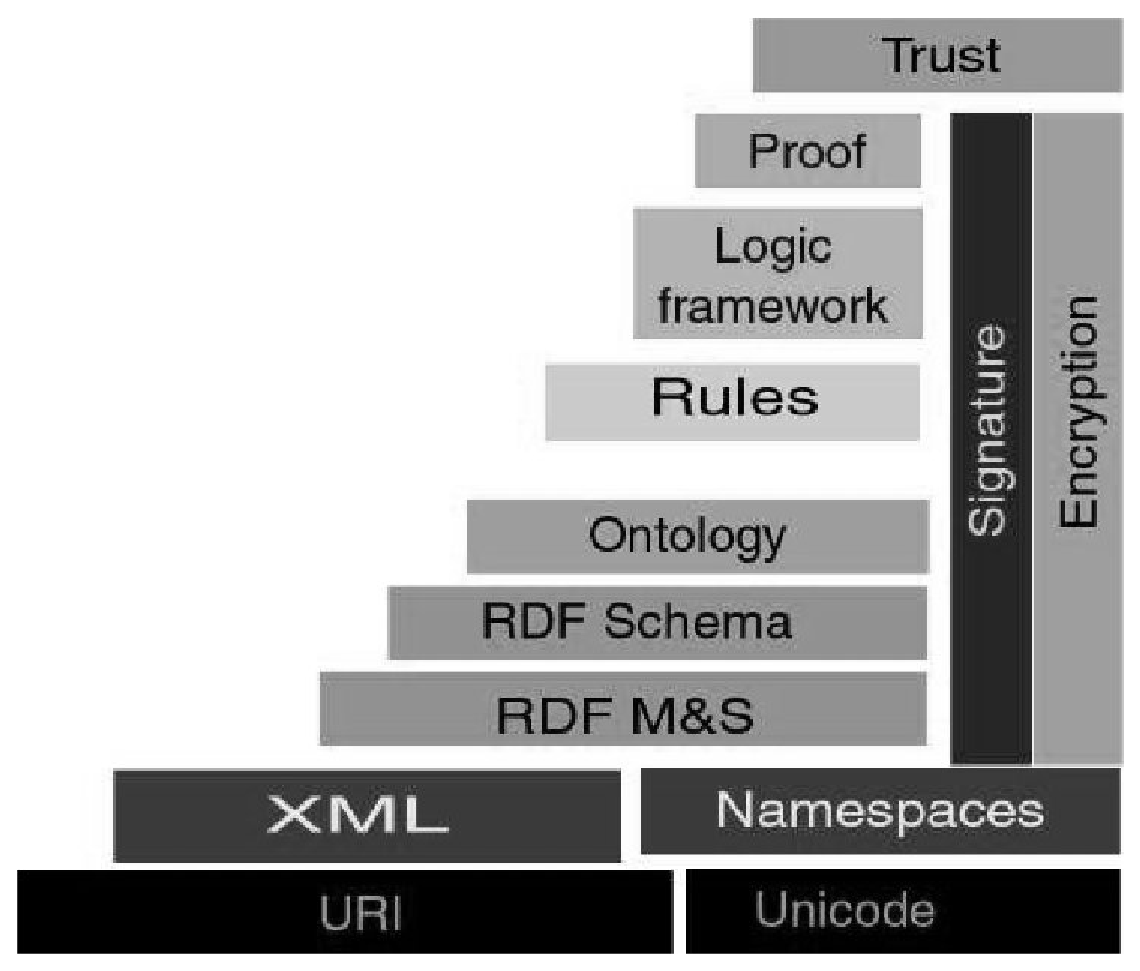
\includegraphics[width=10cm]{images/sw-stack-2002}
\caption{Arquitectura Web Semántica 2002.}
\label{fig:stack-2002}
\end{figure}

A continuación se explica someramente la intención de cada una de las capas y el por qué
de su presencia:
\begin{description}
\item[\gls{URI}/\gls{IRI}-Unicode.] Para dar un soporte estándar a una tecnología existen
dos factores fundamentales: nombrado e identificación única de cada uno de los
recursos y codificación de los mismos. Por esta doble razón aparecen los \textit{Unified
Resource Identifier}y la codificación estándar Unicode, implementada principalmente en UTF-8.
\begin{example}
URI: protocolo:dirección:directorio:recurso, \url{http://www.josemalvarez.es/foaf.rdf}
\end{example}

\item[\gls{XML}~\cite{XML11}.] lenguaje extensible de marcas (\textit{eXtensible Markup
Language}) es un formato estándar creado para la estructuración de datos.
Hoy en día se encuentra regulado por el \gls{W3C} que es el encargado de realizar las distintas
especificaciones y versiones desde Febrero de 1998. XML está basado en \gls{SGML}
(\textit{Standard Generalized Markup Language}, ISO 8879) que ya había sido establecido
en 1986. El uso principal de XML es la estructuración de datos, pero en general es utilizado por todas
aquellas aplicaciones informáticas en las cuales se pueda representar la información jerárquicamente.
El lenguaje XML es en sí mismo un metalenguaje utilizado ampliamente para definir otros
lenguajes. Consta entre otros, de elementos y atributos. Su orden y jerarquía
son los encargados de formar el lenguaje que definimos con XML. No se dispone de etiquetas predefinidas, como podría ser \gls{HTML}, esto
se deja a labor del usuario que es el encargado de definir un conjunto de elementos con sus
etiquetas asociadas, la semántica de los documentos es proporcionada por la aplicación que use
esos datos. Para definir la estructura de un documento XML, es decir, una 
gramática que indique el orden de los elementos y su jerarquía, lo podemos conseguir de
dos formas utilizando: 1) \gls{DTD} o 2) \gls{XML Schema}~\cite{XMLSchema}.

Es importante resaltar que un documento bien formado no es lo mismo que un documento
válido, un documento estará bien formado cuando siga las reglas sintácticas de
formato XML, mientras que un documento será válido si todos sus elementos están en orden correcto de anidación y está bien formado. Algunas de las razones 
por las que es interesante utilizar XML son las siguientes:
\begin{itemize}
\item Estándar para el intercambio de datos.
\item Facilidad de uso.
\item Legibilidad.
\item Implantación.
\item Extensibilidad.
\item Separación entre formato y contenido.
\item Tratamiento multiplataforma.
\item Es libre, especificaciones disponibles. 
\end{itemize}

\begin{figure}[!htbp]
\centering
\lstinputlisting[language=XML]{examples/events.xml}
\caption{Ejemplo de fichero XML.}
\label{fig:ejemplo-xml}
\end{figure}

Como aplicación práctica de XML, ver Figura~\ref{fig:ejemplo-xml}, y debido a la necesidad de tratamiento
automático para diferentes fines (formatos de presentación, transformación de un
vocabulario a otro, etc.) hay que destacar \gls{XSL}~\cite{XSL} generación del
contenido a partir de un documento XML de una manera rápida, sencilla y eficaz, cuyo objetivo principal es presentar al usuario final un 
interfaz del documento más entendible con el que pueda realizar un tratamiento de la información contenida en él de una manera más
asequible, sin necesidad de conocer el formato XML.

\begin{figure}[!htbp]
\centering
	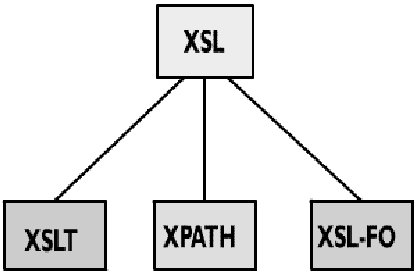
\includegraphics[width=6cm]{images/xsl}
\caption{Componentes de XSL.}
\label{fig:xsl}
\end{figure}

Por ello desde el consorcio \gls{W3C} se optó por realizar la especificación XSL con
el objetivo de presentar un modelo para el procesamiento de la información
almacenada en formato XML. La especificación redactada por el consorcio web para la transformación del contenido XML
se denomina XSL, se encarga de definir una hoja de estilo con la cual se transforma el fichero
XML en otro formato, teniendo en cuenta que la información en XML se almacena de forma
jerarquizada, con la definición de XSL se pretende poder presentar al usuario dicha información
en otros formatos estructurados como pueden ser: HTML, \gls{PDF}, etc., XSL es una especificación, pero 
el lenguaje del que hace uso para la realización de la transformación es XSLT con sintaxis de XPath~\cite{XPath}.

En \gls{XSLT} se define cómo se ha de realizar la transformación del documento XML y no
cuándo se debe realizar, la transformación del documento se realiza en distintos
pasos: 
\begin{itemize}
    \item Generación de un árbol a partir del fichero fuente de XML, esto se
    realiza mediante un procesador que analiza el documento, realizando al mismo tiempo una validación sintáctica del
mismo.
\item Procesamiento del árbol generado construyendo un nuevo árbol con la
información procesada, el recorrido del árbol generado se realiza en preorden, con la posibilidad de variar el tipo de recorrido, es importante tener en cuenta
el orden de evaluación de los nodos del árbol para así poder aplicar las
plantillas correctamente. 
\end{itemize}

El principal uso de XSLT como ha quedado patente en la introducción, es la transformación
de documentos XML para generar contenido web, lógicamente esto no aportaría demasiada potencia
a este lenguaje si solo sirviera para generar contenido web estático. En cambio usando
este lenguaje se genera contenido dinámico aplicando distintas reglas, como ejemplo se
podría obtener de una base de datos un fichero XML y con dicho fichero y una transformación
apropiada generar una página dinámica con contenidos auto-actualizables cada cierto tiempo, otro 
ejemplo de aplicación podría ser la conversión de un programa escrito en un lenguaje a otro, definiendo las reglas correctas. 
XSLT utiliza también \gls{XPath}, ver Figura~\ref{fig:xsl-example}, que es una especificación
para el acceso a los valores de los distintos nodos del árbol generados a partir del procesamiento
del fichero XML. 

\begin{figure}[!hbp]
\centering
\lstinputlisting[language=XML]{examples/events.xsl}
\caption{Ejemplo de hoja de estilo XSL.}
\label{fig:xsl-example}
\end{figure}


\item[\gls{XML Schema}~\cite{XMLSchema}.] En primer lugar es interesante diferenciar las dos
tecnologías establecidas para la definición de la estructura de un documento
XML: \begin{inparaenum}
     \item \textit{Document Type Definition} (\gls{DTD}) es un vocabulario para definir las
     reglas de construcción de un documento XML.     
     \item XML Schema: Vocabulario XML utilizado para definir otros vocabularios
     XML.  
     \end{inparaenum}

El incremento en el uso de \gls{XML} hace necesario la utilización de tecnología para poder
expresar la estructura del documento y así proceder a su validación. Aunque en principio el objetivo de ambos es el mismo: 
definir vocabularios XML para poder validarlos sintácticamente e imponer distintos tipos de 
restricciones como de cardinalidad o integridad, cada uno presenta unas características diferentes 
lo que supone que escoger entre uno u otro implique realizar un estudio de lo que se pretende desarrollar.
También disponemos de herramientas que nos permiten realizar la transformación de uno a
otro pero sólo en el sentido de DTD a XML Schema. Se puede pensar que XML Schema es el
sucesor de las DTD.

La utilización de XML Schema, ver Figura~\ref{fig:xsd-example}, se apoya en diferentes características que hacen
que su uso sea interesante en el ámbito de la Web Semántica:
\begin{itemize}
\item Espacios de nombres, permite utilizar los mismos identificadores en el
mismo documento, evitando así la ambigüedad.
\item Esquema, es la estructura que va a presentar el vocabulario XML construido, con
sus distintos elementos y atributos así como con las validaciones que sean
necesarias.
\item Documento instancia,  documento XML creado con una estructura
definida en un XML Schema y contra el cual se ``valida''.
\end{itemize}

Las razones que pueden llevar a elegir XML Schema son, entre otras, las siguientes:
\begin{itemize}
  \item Utiliza sintaxis XML.
  \item Perfectamente documentado.
  \item Define los elementos y atributos que pueden aparecer en un documento instancia.
  \item Establece la jerarquía y orden de los distintos elementos.
  \item Podemos crear distintos tipos genéricos.
  \item Extensible.
  \item Inclusión de documentos externos.
  \item Expresividad.
  \item Posibilidad de documentación.
  \item Tipos de datos simples, complejos, derivados.
  \item Expresión de restricciones de integridad y cardinalidad.
  \item Reutilización de tipos por extensión o restricción.
  \item \ldots  
\end{itemize}


\begin{figure}[!htbp]
\centering
\lstinputlisting[language=XML]{examples/events.xsd}
\caption{Ejemplo de XML Schema.}
\label{fig:xsd-example}
\end{figure}


La utilización de XML Schema es crítica en los servicios web basados en \gls{WSDL}~\cite{WSDL20} y \gls{SOAP}~\cite{SOAP11} y 
está muy asentada en entornos de desarrollo basados en Java a través de herramientas como \gls{JAXB}.

\item[\gls{RDF}~\cite{RDF}.] \textit{Resource Description Framework}, se encarga
de describir los recursos, añadiéndoles la metainformación necesaria en
un formato procesable. En la siguiente Sección~\ref{rdf} abordaremos la descripción de
RDF de manera más extensa.

\item[Ontologías:] Los documentos etiquetados constituyen una gran cantidad
de información disponible para utilizar por la máquina. Están disponibles los datos, pero
todavía no hay capacidad semántica. Es necesario construir un modelo donde ``encajar''
esos datos. Para añadir la componente semántica mediante ontologías, ver Sección
\ref{ontologias}, se pueden utilizar diferentes lenguajes, cuyo estudio se 
abordará en la Sección~\ref{lenguajes}.

\item[Capas superiores:] La arquitectura propone diferentes niveles en los
que se colocan las reglas y la lógica, debido a su complejidad todavía es precipitado definirlas por completo y las discusiones se mantienen
abiertas en grupos de trabajo del \gls{W3C} como el \gls{RIF}~\cite{rif-core}. 
Los módulos transversales de ``firma''~\cite{XML-dsig} y 
``encriptación''~\cite{XML-enc} están definidos y se
pueden encontrar como recomendaciones del W3C.

\end{description}

Aunque las ventajas de un diseño basado en capas está sobradamente demostrado en
bibliografía de ingeniería del \textit{software}, hay que resaltar que esta primera
aproximación ha sido modificada con el objetivo de recoger la realidad de la
arquitectura para la Web Semántica. Hay que tener en cuenta que la primera
versión propuesta por \textit{Tim Berners Lee} (web XML) ofrecía una visión ideal
que contemplaba todas las partes implicadas, pero que no tenía el efecto experiencia
de la construcción de aplicaciones y de los posibles problemas que se podrían
encontrar. Por ello, esta arquitectura ha sido rediseñada planteando un modelo
más cercano a la realidad, por lo menos de las aplicaciones y problemas, y que
también es conocida como las ``dos torres''~\cite{kifer05} (web RDF), ver Figura~\ref{fig:stack-2005}.

\begin{figure}[!htbp]
\centering
	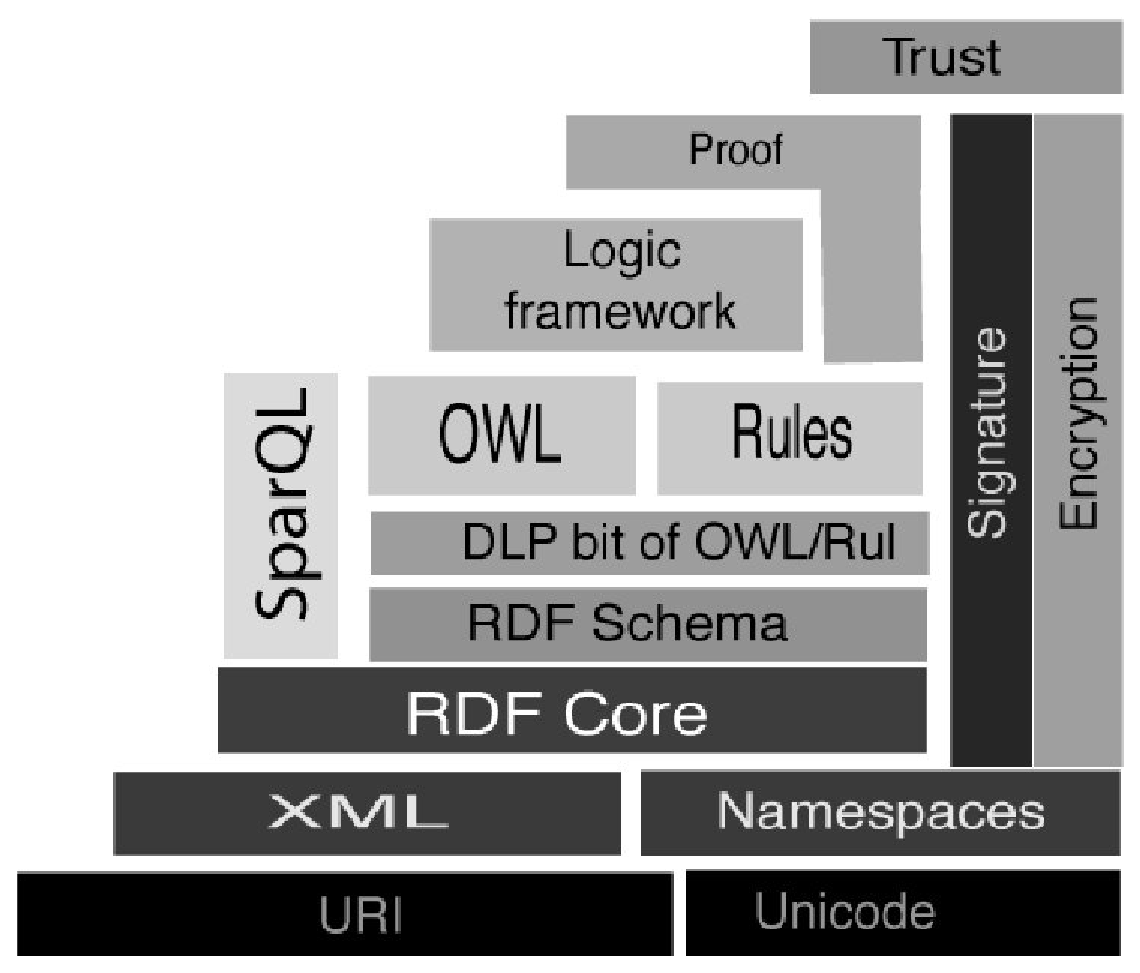
\includegraphics[width=10cm]{images/sw-stack-2005}
\caption{Arquitectura Web Semántica 2005.}
\label{fig:stack-2005}
\end{figure}

La propuesta de cambio surge porque la Lógica Descriptiva, que utiliza \gls{OWL}, no
tiene un poder expresivo suficiente para solucionar el problema de la
representación de conocimiento y razonamiento en la Web Semántica. OWL no puede
tratar con información de una forma dinámica, no tiene predicados \textit{n-arios}, no
soporta símbolos de función, etc. De ahí que se valorará la posibilidad de extender las bases
de conocimiento en OWL con reglas para aumentar la expresividad de los modelos y
ganar en capacidad de inferencia.

Las reglas, en programación lógica como PROLOG, tienen una larga tradición en
las ciencias de la computación y se llevan estudiando desde hace más de 20 años. Sin
embargo, la extensión de OWL con reglas no es una tarea sencilla. En general, las reglas 
están basadas también en un subconjunto de la lógica de primer orden, la
lógica \textit{Horn}, aunque su semántica formal es diferente, no está basada en teoría de modelos. La diferencia fundamental, aparte del tratamiento
de la negación y cuestiones de expresividad, tiene que ver con OWL, ya que, 
debido a su semántica de primer orden, utiliza la hipótesis de mundo abierto,
mientras que las reglas habituales de programación lógica utilizan mundo cerrado. 

La extensión más conocida de OWL en este sentido es \gls{SWRL}~\cite{Swrl}, que permite cláusulas
Horn como axiomas en las bases de conocimiento en OWL. Este lenguaje mantiene
el mundo abierto de OWL, pero penaliza en rendimiento debido a su alto coste computacional.

Debido a esta serie de problemas, se ha sugerido la opción de separar ontologías y
reglas (lógica descriptiva y programación lógica) y utilizar cada tecnología en casos
de uso pertinentes y apropiados. La combinación entre ambos, un objetivo verdaderamente ambicioso de la Web Semántica, 
ya no sería mediante la extensión de OWL con algún tipo de formalismo para la expresión de reglas, sino mediante la construcción
de un interfaz lógico que permita desde las reglas utilizar información definida
en las ontologías, y desde éstas, información inferida por el
comportamiento de los sistemas de reglas.

Destacar la aparición del lenguaje de consulta para RDF, \gls{SPARQL}~\cite{Sparql} y su última
versión SPARQL 1.1, creado por la necesidad de disponer de un lenguaje de acceso a los recursos
definidos en forma de grafo y con una semántica definida~\cite{Perez:2009:SCS:1567274.1567278}. El modelo semántico~\cite{citeulike:1556975} 
proporcionado por RDF permite tratar cualquier recurso como una entidad con descripción asociada. No obstante, el uso de RDF no es
suficiente para la elaboración de modelos de dominio más ricos y descriptivos, razón por la cual surge un lenguaje como OWL que apoyado sobre el modelo de RDF
permite realizar formalizaciones utilizando diferentes lógicas (principalmente \textit{Description Logics}).

\subsubsection{Lenguajes para la Web Semántica: Creando ontologías}\label{lenguajes}
La construcción de una base de conocimiento~\cite{GruberOnto} utilizando ontologías puede
realizarse con distintos lenguajes y diferentes grados de expresividad lógica~\cite{HoPa10a,Kifer:1989:FHL:66926.66939}.
La selección de la lógica apropiada para la modelización de nuestra base de
conocimiento no es una cuestión sencilla y debemos contemplar diferentes
factores: grado de computabilidad, decidibilidad, soporte razonadores, etc.
Todos ellos determinarán la lógica a utilizar ya que no se puede señalar arbitrariamente que se debe utilizar un nivel lógico cuando no es necesario para
el modelo formal.
\subsubsection{RDF}\label{rdf}
El primer lenguaje que nos encontramos para la creación de ontologías es \gls{RDF}
(\textit{Resource Description Framework}) como soporte básico a la par que potente, 
para añadir semántica a los recursos (documentos entre otros). La primera observación 
a realizar es la distinción entre: \begin{inparaenum}\item Modelo de datos, basado en
tripletas Sujeto-Predicado-Objeto. \item Formato de datos, puede utilizar RDF/XML (normativo)
como formato para la serialización del modelo.\end{inparaenum}

El modelo de datos de RDF utiliza tripletas, ver Figura~\ref{fig:rdf-model}, encargadas de describir recursos:
\begin{description}
\item[Sujeto:] recurso sobre el que vamos a realizar una afirmación. Están
identificados de forma única a través de URIs. Por ejemplo: Yo.
\item[Predicado:] es la afirmación sobre el sujeto. Por ejemplo: ``tengoNombre''.
\item[Objeto:] valor del predicado para este sujeto. Por ejemplo: ``Jose
María''@es.
\end{description}

\begin{figure}[!htbp]
\centering
	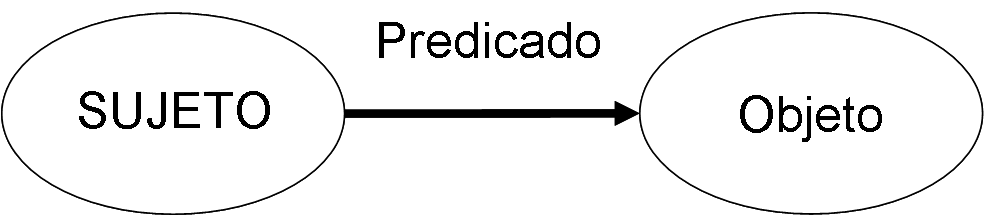
\includegraphics[width=10cm]{images/rdf-model}
\caption{Modelo de tripletas RDF.}
\label{fig:rdf-model}
\end{figure}

Usando RDF pueden realizarse afirmaciones simples sobre ``cosas'': ``Este
documento de memoria tiene de creador'' a ``Jose María Alvarez'' puede expresarse en
RDF usando la tripleta (memoria, ``tieneCreador'', ``Jose María Alvarez''). 
A su vez  se pueden generar nuevas tripletas (memoria, ``tieneFecha'',
``Enero 2012'') o (memoria, ``tieneFormato'', ``PDF''), generando así un
modelo semántico simple pero perfectamente válido. Si se le añade el uso de colecciones y 
la capacidad de ``reificación'' (afirmaciones sobre otras
afirmaciones) se conseguirá una capacidad de expresión muy potente asentada en un
sencillo lenguaje. En cuanto, a la serialización de RDF o su formato, existen diferentes estándar
perfectamente válidos para su tratamiento automático por las máquinas y más o
menos amigables para los humanos. 
\begin{itemize}
  \item \gls{RDF/XML}~\cite{rdf-syntax} formato estándar y normativo por excelencia, ver Figura~\ref{fig:rdf-n3}. 
\begin{figure}[!htbp]
\centering
  \begin{lstlisting} 
<rdf:RDF xmlns:rdf="http://www.w3.org/1999/02/22-rdf-syntax-ns#"
  xmlns:rdfs="http://www.w3.org/2000/01/rdf-schema#"
  xmlns:dc="http://purl.org/dc/elements/1.1/">
    <rdf:Description rdf:about="http://petra.euitio.uniovi.es/~i1637566/">
      <dc:creator>Jose M. Alvarez</dc:creator>
    </rdf:Description>
</rdf:RDF>  
  \end{lstlisting} 
\caption{Ejemplo de tripletas de RDF en RDF/XML.}
\label{fig:rdf-n3}
\end{figure}  

\item Otros como: \gls{RDFa}~\cite{rdfa-primer}, \gls{Turtle}~\cite{turtle-syntax}, \gls{N3}~\cite{n3-syntax} ,\gls{RDF}/\gls{JSON}~\cite{rdf-json} o RDF binario~\cite{rdf-binario}.   
\begin{figure}[!htbp]
\centering
  \begin{lstlisting} 
@prefix dc <http://http://purl.org/dc/elements/1.1/>
<http://petra.euitio.uniovi.es/~i1637566/> dc:creator "Jose M. Alvarez"
  \end{lstlisting}
\caption{Ejemplo de tripleta de RDF en N3.}
\label{fig:rdf-n3}
\end{figure}


 \end{itemize}

En definitiva, RDF provee un mecanismo muy útil para describir recursos que
no realiza presunciones sobre un dominio y capaz de representar a cualquiera
de ellos. La declaración de propiedades (atributos) y su valor semántico se definen
en el contexto de RDF con RDFS (\textit{\gls{RDF Schema}}). RDFS se construye por
encima de RDF y sirve, no solo para definir las propiedades del recurso, sino también
el tipo de recurso. Se pueden crear \textit{clases de recursos}, restringir
combinaciones de las clases, de las relaciones, además de ser el primer nivel de
semántica que permite detectar estas aserciones. RDFS está basado en el
metamodelado de objetos, el principal problema lo constituye la posibilidad de que una
misma clase pueda desarrollar un doble rol de clase o de instancia. Aunque se puede utilizar como
un lenguaje de ontologías desde el punto de vista del manejo de clases, propiedades, rangos y dominios sobre propiedades. 
La posibilidad de generación de jerarquía de conceptos es un lenguaje muy limitado para la expresión de datos en
detalles y no asegura la computabilidad. Es interesante conocer algunos de los vocabularios RDF, especialmente
con el advenimiento de la iniciativa de \linkeddata, que se han creado con distinto propósito, con muy buena 
acogida en la comunidad de Internet y cada día con un uso más extendido: 

\begin{description}
\item[\textit{Dublin Core}.] Vocabulario RDF con las propiedades más comunes y semántica bien definida para el etiquetado de cualquier documento.

\begin{itemize}
  \item Cada etiqueta es opcional y puede estar repetida. Un documento no
  necesita tener resumen y puede tener varios autores.
  \item La mayoría de etiquetas tienen cualificadores para refinar (nunca extender) su significado.
Por ejemplo, la etiqueta ``fecha'' tendrá como cualificadores ``de publicación'',
``de creación'', etc.
\item Principio del Uno-a-Uno. Los metadatos se refieren a un documento
concreto, no a lo representado. 
\item  Principio del \textit{Dumb-down}: Si no se procesan las restricciones al
significado de las propiedades, estas deben seguir proporcionando información
útil. Se pierde nivel de detalle, pero la información sigue siendo válida.
\item Las buenas prácticas de uso para una etiqueta determinada pueden variar por
el contexto. El creador no puede dar por supuesto que serán interpretadas exclusivamente por
una máquina. Esto impondrá algunas restricciones a como se construyen los
metadatos, pero no se debe eludir que el requisito fundamental de
estos es su utilidad para descubrir información.
\end{itemize}

Usando estos principios, \textit{Dublin Core} se impuso el objetivo de lograr un lenguaje
de etiquetado: simple y fácil de mantener, semántica esencial y de significado común, alcance internacional y extensible.
Podemos establecer dos escenarios muy habituales en el uso de este vocabulario:
\begin{enumerate}
  \item En los metaelementos presentes en \gls{HTML} y \gls{XHTML}, ver Figura~\ref{fig:html-dc-example}.

\begin{figure}[!htbp]
\centering
  \begin{lstlisting} 
  <head>
<title>Dublin Core Metadata Initiative (DCMI)</title>
<link rel="schema.DC" href="http://purl.org/dc/elements/1.1/" />
<meta name="DC.title" content="Dublin Core Metadata Initiative (DCMI) Home Page" />
<meta name="DC.description" content="The Dublin Core Metadata Initiative is an open forum . . . metadata standards and practices." />
<meta name="DC.date" content="2011-10-01" />
<meta name="DC.format" content="text/html" />
<meta name="DC.contributor" content="Dublin Core Metadata Initiative" />
<meta name="DC.language" content="en" />
</head>  
 \end{lstlisting} 
\label{fig:html-dc-example}
\caption{Ejemplo de \textit{Dublin Core} en HTML/XHTML.}
\end{figure}
 
\item En documentos RDF propiamente dichos como metadatos de los recursos. A
continuación, se puede ver en la Figura~\ref{fig:rdf-dc-example} el uso de \textit{Dublin Core} en combinación con \gls{RSS}.

\begin{figure}[!htbp]
\centering
\begin{lstlisting}
<rdf:RDF
 xmlns:rdf="http://www.w3.org/1999/02/22-rdf-syntax-ns#"
 xmlns="http://purl.org/rss/1.0/"
 xmlns:dc="http://purl.org/dc/elements/1.1/"
 xmlns:syn="http://purl.org/rss/1.0/modules/syndication/"
 xmlns:taxo="http://purl.org/rss/1.0/modules/taxonomy/"
>
<channel rdf:about="http://dublincore.org">
<title>Dublin Core Metadata Initiative</title>
<link>http://dublincore.org/</link>
<description>Making it easier to find information.</description>
<dc:language>en-us</dc:language>
<dc:rights>1995-2007</dc:rights>
<dc:date>2007-10-01</dc:date>
<items>
<rdf:Seq>
  <rdf:li rdf:resource="http://dublincore.org/news/2007/#dcmi-news-20071001-01" />
  <rdf:li rdf:resource="http://dublincore.org/news/2007/#dcmi-news-20071001-02" />
  <rdf:li rdf:resource="http://dublincore.org/news/2007/#dcmi-news-20071001-03" />
  <rdf:li rdf:resource="http://dublincore.org/news/2007/#dcmi-news-20071001-04" />
</rdf:Seq>
</items>
</channel>

</rdf:RDF>
 \end{lstlisting} 
\label{fig:rdf-dc-example}
\caption{Ejemplo de \textit{Dublin Core} con RDF.}
\end{figure}

\end{enumerate}

\item[\gls{SKOS}-Core~\cite{SKOS-Core}.] Vocabulario RDF utilizado para la representación de conocimiento 
de forma simple a través de conceptos, para ser procesado por máquinas de forma
automática: vocabularios controlados, taxonomías, tesauros, esquemas
conceptuales, glosarios o esquemas categorizados. Algunas de las propiedades de SKOS que 
confieren interés este vocabulario:
\begin{itemize}
\item Identificación de conceptos a través de URIs.
\item  Etiquetado de conceptos: \textit{prefLabel}, \textit{altLabel},
\textit{prefSymbol}, \textit{altSymbol}, etc.
\item Descripción y documentación (conceptos): \textit{definition}, \textit{example}, \textit{scopeNote},
\textit{version}, \textit{changeNote}, etc.
\item Relaciones entre conceptos: \textit{broader}, \textit{narrower},
\textit{related}, etc. 
\item Indexación: \textit{subject}.
\item Soporte multiling\"{u}e
\end{itemize}

En la siguiente Figura~\ref{fig:skos} se presenta un ejemplo más completo del
uso de SKOS-Core para la descripción de conceptos:
 
\begin{figure}[!htbp]
\centering
	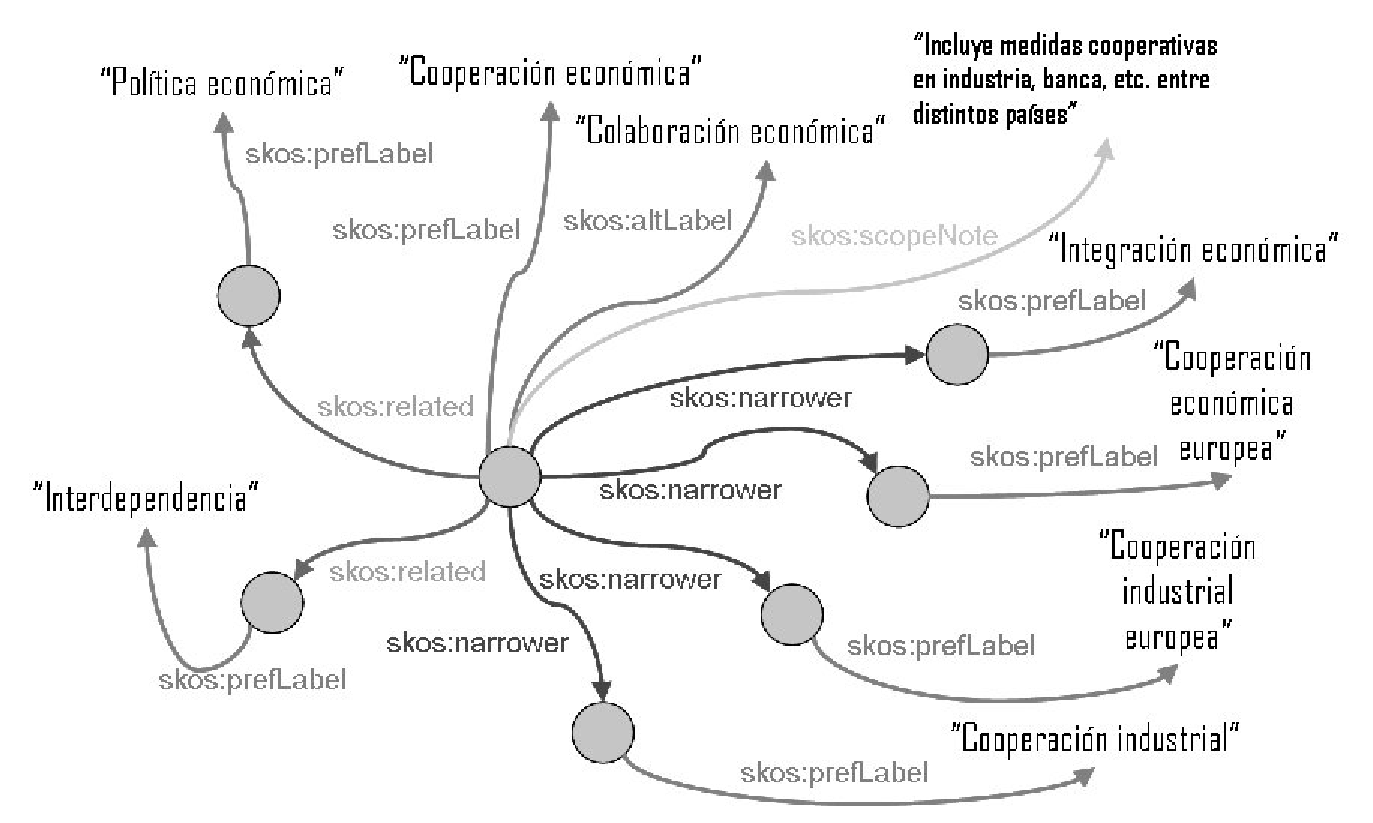
\includegraphics[width=14cm]{images/skos}
\caption{Concepto expresado en SKOS-Core.}
\label{fig:skos}
\end{figure}

Debe puntualizarse que el uso de SKOS-Core está siendo objeto de estudio para la
representación de recursos lexicográficos~\cite{Milin} desde un punto de vista de la
lingüística y como un avance tecnológico en este campo.

\item[\gls{FOAF} y \gls{DOAP}.] Vocabularios RDF para definir personas y amistades (\textit{Friend Of A Friend}), ver Figura~\ref{fig:foaf-example}, o 
proyectos (\textit{Description Of A Project}), 
ver Figura~\ref{fig:doap-example}. Cada vez hay un mayor interés por este tipo de tecnologías y algunos proyectos de gran envergadura como 
Apache o RDF Ohloh~\cite{Ferndez08rdfohloh}, que incluyen muchos subproyectos, programas, etc., utilizan estas
descripciones semánticas para cada módulo.

\begin{figure}[!htbp]
\centering
  \begin{lstlisting}
<#me> a foaf:Person;
	foaf:family_name "Alvarez Rodr\u00EDguez";
	foaf:givenname "Jose Mar\u00EDa";
	foaf:homepage <http://josemalvarez.es>;
	foaf:knows _:bnode2016979200;
	foaf:mbox_sha1sum "0d1d9ad2de64fd900d03c18e3d2608171832d155";
	foaf:name "Jose Mar\u00EDa Alvarez Rodr\u00EDguez";
	foaf:nick "chema";
	foaf:phone <tel:+34-666-714-721>;
	foaf:schoolHomepage <http://www.uniovi.es/inicio/>;
	foaf:title "Sr.";
	foaf:workplaceHomepage <http://www.weso.es>.
_:bnode2016979200 a foaf:Person;
	rdfs:seeAlso <http://www.di.uniovi.es/~labra/labraFoaf.rdf>;
	foaf:mbox_sha1sum "5fa5d69bac0c1396825c475ec19325ec0ffd5569";
	foaf:name "Jose Emilio Labra".
  \end{lstlisting}
\caption{Ejemplo parcial de documento FOAF en N3.}
\label{fig:foaf-example}
\end{figure}


\begin{figure}[!htbp]
\centering
  \begin{lstlisting}
<http://rdfohloh.wikier.org/project/moldeas/rdf> 
	dct:isFormatOf 	<http://rdfohloh.wikier.org/project/moldeas>;
	a foaf:Document;
	rdfs:label "MOLDEAS's DOAP document serialized in RDF/XML";
	foaf:primaryTopic <http://rdfohloh.wikier.org/project/moldeas>.
	<http://rdfohloh.wikier.org/project/moldeas> dct:updated "2012-01-22T13:02:25Z";
	rdfohloh:ohloh-page <http://www.ohloh.net/projects/moldeas>;
	doap:created "2011-10-14T09:19:11Z";
	doap:description "This work aims to apply the semantic web and 
	    LOD approaches to public procurement notices...";
	doap:download-page <http://code.google.com/p/moldeas/downloads/list>;
	doap:homepage <http://purl.org/weso/moldeas/>;
	doap:name "MOLDEAS";
	doap:programming-language "JavaScript";
	a doap:Project;
	= <http://rdfohloh.wikier.org/project/586667>;
	skos:subject <http://dbpedia.org/resource/Java>, 
	<http://dbpedia.org/resource/JavaScript>.
  \end{lstlisting}
\caption{Ejemplo parcial de documento DOAP en N3.}
\label{fig:doap-example}
\end{figure}

\item[\gls{SIOC}.] (\textit{Semantically-Interlinked Online Communities}). Es una ontología desarrollada 
por el equipo de Web Semántica de DERI Galway para describir semánticamente
distintas comunidades \textit{online}. SIOC integra, ver Figuras~\ref{fig:sioc} y~\ref{fig:sioc-example}, distintos vocabularios RDF con el
objetivo de reutilizar las definiciones ya realizadas en \gls{FOAF}, \gls{SKOS},
\gls{RSS} o \textit{Dublin Core}. Se ha empleado con éxito en distintas aplicaciones para gestionar y
describir toda la información disponible de las comunidades \textit{online}: listas de correo (SWAML~\cite{Sergio}), 
foros, etc.
 
\begin{figure}[!htb]
\centering
	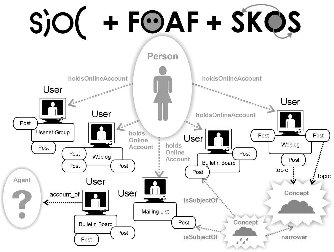
\includegraphics[width=12cm]{images/sioc}
\caption{SIOC integración con otros vocabularios.}
\label{fig:sioc}
\end{figure}

\begin{figure}[!htbp]
\centering
  \begin{lstlisting}
<rdf:RDF
  xmlns:sioc='http://rdfs.org/sioc/ns#'
  xmlns:rdf='http://www.w3.org/1999/02/22-rdf-syntax-ns#'
  xmlns:dc='http://purl.org/dc/elements/1.1/'
  xmlns:mvcb='http://webns.net/mvcb/'
>
  <sioc:Site rdf:about="http://groups.google.com/group/sioc-dev">
    <sioc:host_of>
      <sioc:Forum rdf:about="http://swaml.berlios.de/demos/sioc-dev/index.rdf#SIOC-Dev">
        <dc:description>SIOC development mailing list</dc:description>
        <mvcb:errorReportsTo rdf:resource="http://swaml.berlios.de/bugs"/>
        <sioc:container_of rdf:resource="http://swaml.berlios.de/demos/sioc-dev/2006-Dec/post-419.rdf"/>
        <dc:date>2007-06-18</dc:date>
        <dc:title>SIOC-Dev</dc:title>
        <mvcb:generatorAgent rdf:resource="http://swaml.berlios.de/doap.rdf"/>
        <sioc:has_host rdf:resource="http://groups.google.com/group/sioc-dev"/>
        <sioc:has_subscriber rdf:resource="http://swaml.berlios.de/demos/sioc-dev/subscribers.rdf#s26"/>
      </sioc:Forum>
    </sioc:host_of>
  </sioc:Site>
</rdf:RDF>
  \end{lstlisting}
\caption{Ejemplo de descripción con SIOC.}
\label{fig:sioc-example}
\end{figure}

\item[\gls{RSS}.] Existen diferentes versiones y definiciones de este vocabulario RDF, ver Figura~\ref{fig:rss-example}: \textit{Rich Site Summary} (RSS 0.91), XML; 
\textit{RDF Site Summary} (RSS 0.9 y 1.0), RDF; \textit{Really Simple Syndication} (RSS 2.0). La definición
realizada en el \gls{W3C} es la siguiente:

\begin{Frame}
Vocabulario RDF basado en XML que permite la catalogación de información (noticias y eventos) 
de los usuarios. Los archivos RSS contienen metadatos sobre fuentes de información especificadas 
por los usuarios, cuya función principal es notificar de forma automática cualquier cambio que se realice 
en esos recursos de interés.
\end{Frame}

\begin{figure}[!htb]
\centering
\lstinputlisting[language=XML]{examples/rss.rss}
\label{fig:rss-example}
\caption{Ejemplo de canal RSS.}
\end{figure}

\end{description}

En resumen, se dispone de un lenguaje muy útil y sencillo para describir recursos (RDF) y 
un esfuerzo en forma de vocabulario para la definición de recursos más detallada (RDFS) pero incompleto. 
Por ello, a continuación, se expondrán algunos de los lenguajes más completos que han surgido para 
intentar mejorar los puntos débiles de esta primera aproximación para la expresión de modelos semánticos. En cuanto
a vocabularios RDF existen una infinidad~\cite{common-vocabularies} de ellos para ser utilizados en distintos contextos que han sido
enormemente impulsados por la corriente \linkeddata y \opendata.
%Avoiding too many floats 
\clearpage

\subsubsection{OIL}
El \textit{Ontology Inference Layer}~\cite{Fensel01oil:an} (\gls{OIL}) desarrollado en el proyecto Europeo 
\textit{OntoKnowledge} está construido por encima de \gls{RDF} y RDFS utilizando muchos de sus constructores e intentando
mantener la compatibilidad hacia atrás. OIL provee características de modelado
basada en lógica de marcos~\cite{Kifer:1989:FHL:66926.66939} y \textit{Description Logic}~\cite{baader03description}.

La importancia de OIL reside en la unificación de:
\begin{itemize}
\item \textit{Description Logic}, heredando su semántica formal y la capacidad
de razonamiento efectivo (FaCT++, Racer o Pellet).
\item Sistemas basados en marcos, incorpora las características básicas de
modelado basado en marcos (conceptos, superclases, atributos, etc.).
\item Estándares web, construido sobre RDF y RDFS y utilizando como formato de
intercambio de datos XML.
\end{itemize}

Las ontologías creadas con OIL distinguen distintos meta niveles, con el
objetivo de proporcionar distintos niveles de servicio que pueden ser válidos para un
gran número de ontologías y aplicaciones:
\begin{description}
\item[Primer meta nivel:] también conocido como \textit{definición de ontologías}, en la
cual se proveen las definiciones de ontología, terminología que debería ser
instanciada para definir un vocabulario estructurado con la semántica adecuada.
\item[Segundo meta nivel:] conocido como ``meta meta'' nivel o \textit{contenedor de
ontologías}, describe las características de la ontología tales como autor,
nombre, ámbito, etc. Las anotaciones de este nivel se hacen mediante
\textit{Dublin Core}.
\end{description}

La capacidad de razonamiento es otra de las características importantes de OIL, que no estaba presente en RDF. Habitualmente esta capacidad se utiliza
para realizar las operaciones de clasificación, validación de consistencia e inferencia de nuevo conocimiento de acuerdo a distintos 
niveles de expresividad: 

\begin{description}
\item[Core OIL:] prácticamente compatible con RDFS exceptuando la capacidad de
``reificación''.
\item[Standard OIL:] lenguaje que captura las primitivas y constructores necesarios para
construir modelos semánticos con capacidad de inferencia.
\item[Instance OIL:] inclusión de ``instancias''.
\item[Heavy OIL:] capacidades extras de representación y razonamiento.
\end{description}


\begin{figure}[htb]
\centering
	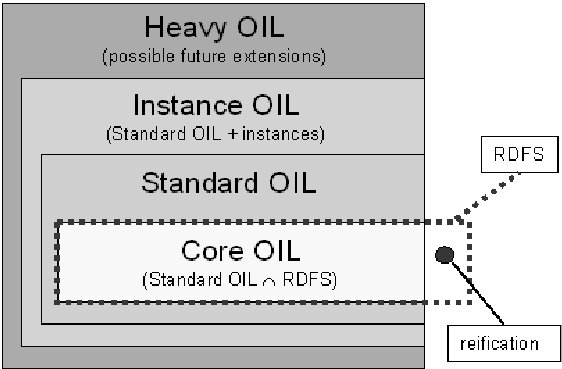
\includegraphics[width=10cm]{images/oil}
\caption{Niveles de expresividad OIL.}
\label{fig:oil}
\end{figure}

Cabe concluir, por tanto, que las principales ventajas de OIL se resumen en:
\begin{inparaenum} \item una aplicación no está obligada a trabajar con un
lenguaje más expresivo de lo necesario. \item aplicaciones que utilicen la
expresividad más baja pueden añadir aspectos de otras ontologías.
\item aplicaciones con un alto nivel de complejidad pueden utilizar
características de otras más simples.\end{inparaenum}

El trabajo realizado en OIL tiene su continuación en el siguiente lenguaje de
modelado de ontologías \gls{DAML+OIL}, ver Figura~\ref{daml+oil}, realizado por la cooperación
de iniciativas europeas y americanas.

\subsubsection{DAML+OIL}\label{daml+oil}
\gls{DAML+OIL}~\cite{HM00} es un lenguaje de marcado semántico para recursos web creado por la cooperación de las iniciativas
europeas (OIL) y americanas (DAML-ONT, \gls{DARPA} \textit{Agent Markup Language})
en el desarrollo de ontologías. El objetivo de desarrollo de este lenguaje está
especialmente centrado para la Web Semántica, modelización de dominios concretos,
utilizando los estándares (\gls{XML} y \gls{RDF}) y añadiendo una serie de primitivas de
orientación a objetos (clases, propiedades, axiomas y aserciones),
sistemas basados en marcos y parte de \textit{Description Logic}. Además, 
DAML+OIL da soporte a los tipos de datos de \gls{XML Schema}, separando las instancias
de una clase y de las instancias de tipos de datos. El significado de DAML+OIL
está definido por un modelo semántico estándar basado en las interpretaciones, consistiendo éstas 
en un dominio del discurso y una función de interpretación.

\subsubsection{OWL}\label{owl}
\gls{OWL}, lenguaje de ontologías para la web, sucesor de DAML+OIL, actualmente está
siendo desarrollado por el W3C, su primera versión estable es OWL 1.0, 
aunque que ya se ha publicado una nueva versión OWL 1.1~\cite{OWL11} y OWL2~\cite{owl2-primer}.

Como lenguaje para ontologías es una potente herramienta que dota de la
expresividad necesaria para mejorar algunos de los servicios más utilizados en
la red de Internet: búsqueda, manejo del conocimiento, interacción entre agentes
automáticos etc. Desde un punto de vista más formal, OWL está formado por
un conjunto de primitivas o constructores de metamodelado que son el punto de
partida para operaciones más complejas, como las de razonamiento. Actualmente,
aunque las características genéricas de OWL tienen su origen en OIL, se distinguen
al menos 3 versiones de OWL (en su versión 1.0 y 1.1) dependiendo de su expresividad, complejidad y grado
de computabilidad, cada versión superior de OWL contiene a la anterior
($Lite\subset DL \subset FULL$).

\begin{description}
\item[OWL-FULL.] Se pueden utilizar todos los constructores y primitivas
definidos en OWL y no restringe el uso de RDF. Esto implica que no se garantiza
su decidibilidad pero en cambio, como familia de \textit{Description Logics}
posee un gran poder expresivo: tratar clases como instancias, definir
propiedades sobre tipos de datos (\textit{string}, \textit{float}, etc.) .

\item[OWL-DL.] Subconjunto decidible de OWL-FULL, supone la máxima expresividad
computable. Cada modelo realizado en OWL-DL genera directamente un modelo
semántico en \textit{Description Logics}.

\item[OWL-Lite.] Añade restricciones adicionales sobre en el uso de los
constructores de OWL, básicamente se pueden modelar jerarquías con restricciones
sencillas.
\end{description}

Para advertir a que nivel de expresividad y complejidad se puede trabajar
dependiendo del lenguaje utilizado se dispone la Figura~\ref{fig:owl-dialects}, extraída del laboratorio OntoText.

\begin{figure}[htb]
\centering
	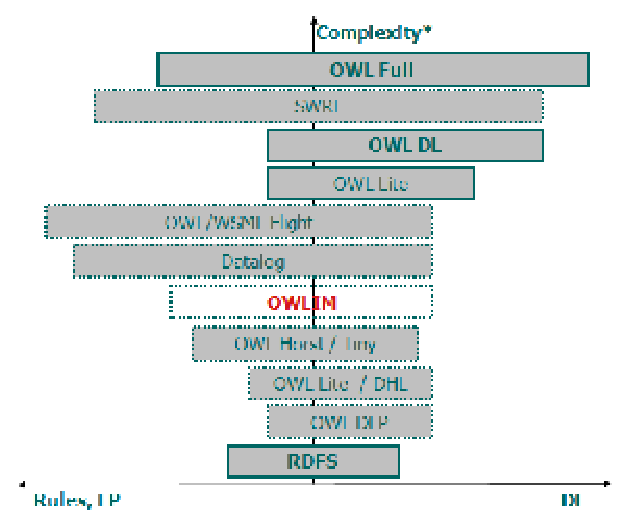
\includegraphics[width=10cm]{images/owl-dialects}
\caption{Algunos lenguajes para la Web Semántica por OntoText.}
\label{fig:owl-dialects}
\end{figure}


Algunas de las características que hacen interesante el uso de OWL en el ámbito
de la Web Semántica son:
\begin{itemize}
  \item Las ontologías en OWL son una serie de axiomas y hechos que pueden
  reutilizar otras ontologías (importándolas). Además, como documento que son
  (serializado en RDF/XML), están identificadas por un URI y tienen asociada cierta metainformación
  (author, dominio, fecha, etc.) que permite que sean referenciables como
  cualquier otro recurso en la red.
  \item Los axiomas son utilizados para asociar una serie de características
  (descripciones, restricciones, etc.) a las clases y propiedades de la
  ontología. 
\item Los hechos proporcionan información particular de una determinada instancia. 
\end{itemize}

Como ejemplo de utilización de OWL, en su versión DL y con características de OWL2, se presenta una sencilla
ontología, ver Figura~\ref{fig:psydiag}, que modela un sistema de diagnóstico psicológico con capacidad de clasificar individuos
de acuerdo a sus síntomas, ver Figura~\ref{fig:psydiag-axiomas}, con sintaxis Manchester.

\begin{figure}[htb]
\centering
	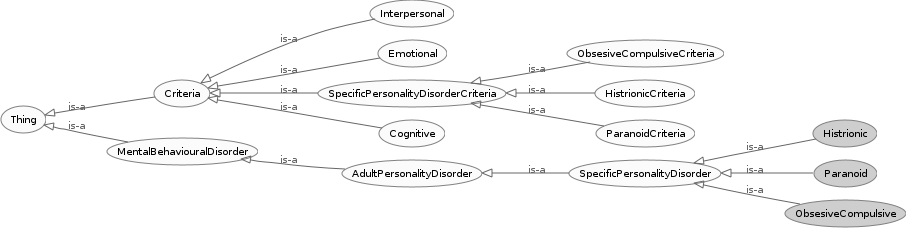
\includegraphics[width=16cm]{images/psydiag}
\caption{Ontología de ejemplo en OWL2 para diagnóstico psicológico.}
\label{fig:psydiag}
\end{figure}


\begin{figure}[htb]
\centering
 \begin{lstlisting} 
Class: <http://example.org/psydiag.owl/Histrionic>

    EquivalentTo: 
        <http://example.org/psydiag.owl/has-criteria> min 3
	      <http://example.org/psydiag.owl/HistrionicCriteria>,
        (not (<http://example.org/psydiag.owl/has-criteria> some 
	      <http://example.org/psydiag.owl/ObsesiveCompulsiveCriteria>))
         and (not (<http://example.org/psydiag.owl/has-criteria> some 
	      <http://example.org/psydiag.owl/ParanoidCriteria>))
         and (<http://example.org/psydiag.owl/has-criteria> only 
	      <http://example.org/psydiag.owl/HistrionicCriteria>)
    
    SubClassOf: 
        <http://example.org/psydiag.owl/SpecificPersonalityDisorder>

DisjointClasses: 
    <http://example.org/psydiag.owl/Histrionic>,
    <http://example.org/psydiag.owl/ObsesiveCompulsive>,
    <http://example.org/psydiag.owl/Paranoid>
  \end{lstlisting} 
\caption{Algunos axiomas de ejemplo en OWL2 para diagnóstico psicológico.}
\label{fig:psydiag-axiomas}
\end{figure}


\subsubsection{WSML}
\gls{WSML}~\cite{WSML2006} es la propuesta de lenguajes formales realizado en \gls{WSMO}~\cite{WSMODeri} 
(relevante por su relación con los Servicios Web Semánticos) para la construcción de ontologías y que recoge 
distintas variantes de lógica, ver Figura~\ref{fig:wsml-layering}. En general, teniendo en cuenta los
distintos tipos de lógica de acuerdo a su expresividad es posible obtener diferentes serializaciones
de los modelos realizados con distintos lenguajes \gls{OWL}, WSML, F-Logic, etc. Esta característica
es muy interesante para el uso de razonadores con distintos tipos de algoritmos y capacidades de
razonamiento, independientemente del lenguaje en el que se haya modelado el dominio.

\begin{figure}[htb]
\centering
	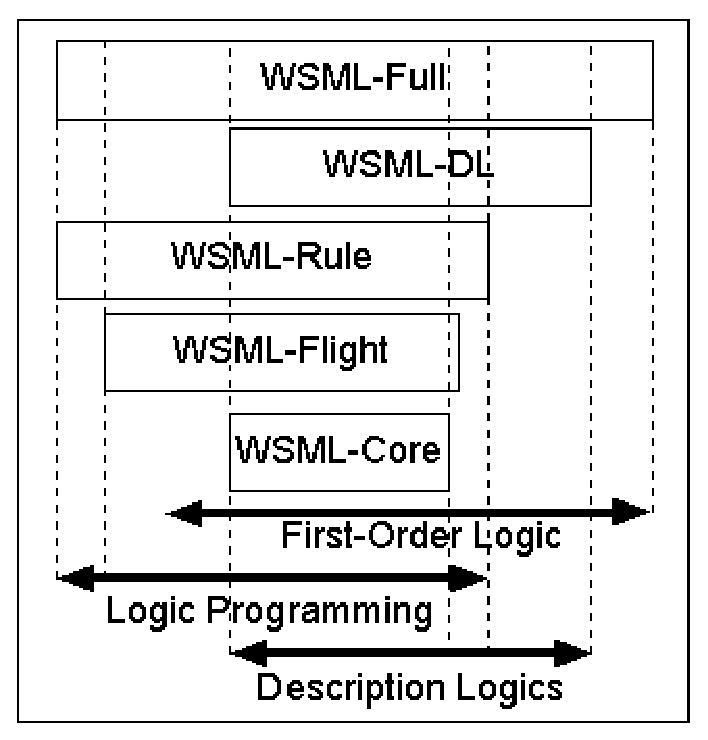
\includegraphics[width=8cm]{images/wsml-layering}
\caption{Capas de WSML.}
\label{fig:wsml-layering}
\end{figure}

\begin{note}
En OWL, con la arquitectura semántica de una torre, ver Figura~\ref{fig:stack-2002}, las
reglas ocuparían una capa por encima del lenguaje. Sin embargo, la práctica ha demostrado que la reglas son
parte de la ontología (no son condición necesaria, pero a un mínimo de complejidad en el
modelo se aprecia su utilidad). WSML incluye una variedad cubriendo esta
posibilidad (WSML-RULE).
\end{note}


\subsubsection{Nota}
Los lenguajes aquí presentados no son los únicos para la expresión de modelos de
conocimiento basados en semántica y reaprovechables para la web. No obstante,
al estar impulsados por el \gls{W3C} y pretender ser estándares, resultan de especial
interés y casi de conocimiento obligado para la comunidad de la Web Semántica.

No se puede determinar cuál es mejor que otro, la decisión de un lenguaje u otro
 debería venir asociado a un profundo análisis tanto funcional: propiedades  del
dominio a modelar y las necesidades lógicas del mismo como no funcional:
herramientas desarrollados, soporte, estabilidad, etc. Actualmente, \gls{OWL} 1.0
en su versión DL, \gls{WSML} y \gls{RDF} están siendo ampliamente utilizados mientras que las
propuestas de \gls{OIL}, \gls{DAML+OIL} y RDFS o bien están obsoletas o no han cumplido
las expectativas de los desarrolladores.


 
                                                           
\subsection{Ontolog\'ias}\label{ontologias}
\subsubsection{Antecedentes y Definición}
El desarrollo de las ontologías se deriva directamente de la filosofía, 
Aristóteles acuña el término ``Categoría'' como palabra para describir las
diferentes clases en las que se dividían las cosas del mundo. 
El término ``ontología'' es relativamente moderno (siglo XIX), proviene del griego
$Ontos$ (Ser) y $Logos$ (Palabra), se empezó a utilizar para diferenciar el
estudio de la Teoría de Categorías que se hacía en biología, de hecho, el trabajo de categorización surge en muchas áreas de la
ciencia (filosofía, biología, medicina, lingüística, etc.).

El cuerpo de un esquema de conocimiento, \textit{lo} que se puede representar, está basado en una
conceptualización: objetos, conceptos y otras entidades, que se asume existen en
un determinado dominio y que mantienen unas relaciones entre sí. 

\begin{Frame}
\textit{Una ontología es una especificación (explícita) de una conceptualización}~\cite{GruberOnto}. 
\end{Frame}

Las ontologías, por consiguiente, son sistemas basados en el conocimiento (\textit{\gls{SBC}}) que
sirven como modelo unificado en la representación del mismo, adquiriendo incluso
grado de ingeniería~\cite{isbn1846283965,Benjamins98ontological}. En muchos
casos, la Web Semántica y por extensión las ontologías se apoyan en la
reutilización de conocimiento compartido. Las definiciones realizadas para las ontologías son variadas y todas dejan claro
que sirven para modelar cierto dominio (conjunto de conceptos y relaciones):

\begin{itemize}
  \item Una ontología define los términos básicos y las relaciones establecidas en cierta área.
  \item Especificación explícita de una conceptualización.
  \item Especificación formal y explícita de una conceptualización compartida.
  \item Teoría lógica que provee de forma explícita y parcialmente una conceptualización.
  \item \ldots
\end{itemize}

En el artículo~\cite{Studer98knowledge} los autores agregan
expresividad realizando la siguiente descripción completa de ontología:
\begin{itemize}
  \item Conceptualización, modelo abstracto de algún fenómeno del mundo,
  proveniente de la identificación de los conceptos relevantes de dicho
  fenómeno. \item Explícita, conceptos y restricciones usados se definen
  explícitamente. \item Formal, capacidad de ser legible e interpretable por las
  máquinas.
  \item Compartida, captura conocimiento consensuado.
\end{itemize}

Es posible fusionar las definiciones anteriores en nueva descripción del término ontología:
\begin{definition}
Modelo conceptual organizado mediante una taxonomía que permite definir
relaciones entre conceptos, funciones, instancias (elementos) y axiomas en un determinado
dominio.
\end{definition}

Para completar la definición de ontología hay que tener en cuenta la
nomenclatura que habitualmente se utiliza para nombrar a las distintas entidades
posibles y que en algunos casos puede dar lugar a errores:

\begin{itemize}
  \item Clase, concepto, categoría o tipo.
  \item Instancia, individual.
  \item Entidad, objeto (clase o instancia).
  \item Propiedad, relación, slot, atributo, rol.
\end{itemize}

En la actualidad, la construcción de sistemas basados en conocimiento conlleva la
creación partiendo de cero de nuevas bases de conocimiento. La aspiración debería ser
utilizar componentes reutilizables~\cite{Gruber93towards}, de esta manera los desarrolladores deberían
crear sistemas con la agregación del conocimiento ya existente. El conocimiento definido, 
las técnicas de resolución de problemas y otros servicios, podrían ser
compartidos entre varios sistemas, impulsando la creación de grandes sistemas con
un bajo coste. Desde esta perspectiva, se pueden usar las ontologías como
infraestructura para sistemas ubicuos.

\subsubsection{Componentes}
Una ontología consta de un conjunto no vacío de conceptos identificados como
relevantes en el dominio a modelar, un conjunto de atributos para describir los
conceptos que pueden proveer de distintas fuentes: propios, heredados, etc., un
conjunto de funciones, un conjunto de axiomas que formalizan las condiciones que
deben cumplir los distintos conceptos y un conjunto de instancias o
realizaciones particulares de los conceptos.

\begin{description}
\item[Conceptos:] cualquier entidad que se puede describir, tiene asociado un
identificador único, puede poseer diferentes atributos y establecer relaciones
con otros conceptos.
\item[Relaciones:] representan la interacción entre los conceptos de dominio.
Formalmente, se definen como subconjuntos del producto cartesiano de $n$
conjuntos $R: C_1 \times C_2 \times \ldots \times C_n$.

No todas las relaciones tienen el mismo significado, existen relaciones binarias
de especialización como (\textit{is-a}) o de composición (\textit{part-whole}),
que se modelan con las propiedades clásicas simétricas, reflexivas, etc.

\item[Funciones:]relaciones en las cuales el elemento \textit{n-ésimo} es único para
los $n-1$ anteriores. Formalmente, se definen como $F:C_1 \times C_2 \times
\ldots \times C_n$. Por ejemplo una relación \textit{serPadreDe} se puede
modelar como una función ya que el atributo que evalúa es único para cada caso.

\item[Axiomas:] modelan ``verdades'' que siempre se cumplen en el modelo.
Existen dos tipos de axiomas:
\begin{itemize}
  \item Estructurales, condiciones relacionadas con la estructura jerárquica de
  la ontología. 
  \item No estructurales, establecen relaciones entre atributos de un concepto y
  son específicos de cada dominio.
\end{itemize}

\item[Instancias:] representan realizaciones específicas del dominio de la ontología.
\end{description}

\subsubsection{$Description Logics$ y ontologías}
\textit{Description Logics}~\cite{baader03description} (\gls{DL}s) son un conjunto de lógicas
formales en el área de \textit{Knowledge Representation}, utilizadas para la representación y
razonamiento del conocimiento en un dominio de forma no ambigua. Las DLs se
basan en una semántica perfectamente definida que provee un conjunto de
constructores y primitivas con un significado lógico preciso.

Los pilares de estas lógicas son dos conjuntos: uno de ellos, \textit{atomic concepts}
o predicados unarios y otro, \textit{atomic roles} o predicados binarios. Una
DL provee además un conjunto de operadores, llamados \textit{constructores}, que
permiten crear conceptos y roles más complejos a partir de los más sencillos.
Tanto los conceptos atómicos como los complejos, se denominan uniformemente \textit{conceptos}
y de igual forma, los roles atómicos y los complejos se denominan
\textit{roles}.

Los conceptos se utilizan para representar conjuntos de objetos y los roles
sirven para establecer relaciones binarias entre objetos. Podemos definir el
conjunto de los números reales como la disyunción de
números racionales e irracionales
\begin{example}
$ \mathbb{R} \equiv \mathbb{Q} \sqcup \mathbb{I}$
\end{example}

En general, una base de conocimiento basada en DL consiste en:
\begin{itemize}
  \item \textit{TBox}, contiene los axiomas de inclusión de conceptos
  $C_1 \sqsubseteq C_2$.
  \item \textit{RBox}, contiene los axiomas de inclusión de roles $R_1 
  \sqsubseteq R_2$.
  \item \textit{Abox}, contiene axiomas (aserciones sobre conceptos) $C(a)$, las
  aserciones sobre los roles $R(a,b)$, $a$ y $b$ son son nombre de objetos, $R$
  es un rol y $C$ es un concepto.
\end{itemize}
 
Los constructores booleanos de conceptos son la $\sqcup$ (disyunción o unión),
$\sqcap$ (conjunción o intersección) y $\neg$ (negación). Una
DL que provee, implícita o explícitamente, todos los operadores booleanos se
considera \textit{cerrada} (proposicionalmente). Las DLs ``cerradas'' serán las
que sean interesantes para su procesamiento en la Web Semántica. Aparte de los
operadores booleanos, habitualmente las DLs proveen otros constructores para
generar conceptos complejos a partir de roles. En este apartado, se encuentran
los operadores existencial ($\exists$)  y universal $\forall$. 

Las DLs que proveen estos cinco operadores se denominan $\mathcal{ALC}$, pero
esta lógica no permite axiomas de inclusión en roles y la componente 
\textit{RBox} es vacía, supone que si bien se pueden realizar operaciones
de razonamiento, la lógica a este nivel es poco expresiva. Añadiendo nuevos
constructores a $\mathcal{ALC}$ se obtiene el conjunto de lógicas
$\mathcal{ALC_{HR^+}}$ (también conocida como $\mathcal{SH}$), que resultan de añadir la
inclusión de axiomas (permitiendo diferentes tipos), sobre la \textit{RBox}.
Esta familia de lógicas, ver Tabla ~\ref{table:sh} extraída de~\cite{Cuenca}, es muy
interesante porque posee un gran poder expresivo y puede ser probada sobre razonadores DL, como FaCT++, Racer, Pellet o Hermit.


\begin{table}[htb]
\renewcommand{\arraystretch}{1.3}
\begin{center}
\begin{tabular}{|c|c|c|}
\hline
\textbf{Nombre constructor}&\textbf{Sintaxis}&\textbf{Lógica}\\
\hline
Concepto atómico& $A$ & \\
Concepto universal& $(\top)$ & \\
Rol atómico& $R$ & \\
Conjunción de conceptos& $C \sqcap D$ & \\
Disyunción de conceptos& $C \sqcup D$ & \\
Negación de concepto& $\neg C$ & \\
Restricción existencial& $\exists R.C$ & \\
Restricción universal& $\forall R.C$ & \\
Rol transitivo& $Trans(R)$ & $\mathcal{S}$\\
\hline
Jerarquía de roles& $R_1 \sqsubseteq R_2$ & $\mathcal{H}$\\
\hline
Inversión de roles& $(R^-)$ & $\mathcal{I}$\\
\hline
Nominales (instancias)& $\{o\}$ & $\mathcal{O}$\\
\hline
Restricciones funcionales de número& $\geq 2S  (\geq 1S)$ &
$\mathcal{F}$\\ \hline

Restricciones no cualificadas de número& $\geq nS  (\leq nS)$ &
$\mathcal{N}$\\ 

\hline

Restricciones cualificadas de número& $\geq nS.C  (\leq nS.C)$ &
$\mathcal{Q}$\\ 

\hline
\hline

\end{tabular}
\caption{Familia de lógicas $\mathcal{SH}$.}
\label{table:sh}
\end{center}
\end{table}

La lógica DL es importante para la construcción de ontologías ya que permite
construir bases de conocimiento formales, computables y no ambiguas. Aunque no siempre será indispensable este nivel 
de lógica, tanto para la descripción de dominios como para la Web Semántica, es necesario presentar y dar a conocer este conjunto
de lógicas, para así validar los modelos y mantener unos criterios
formales en la construcción de ontologías. Las ontologías construidas con lógica
DL proporcionan una base sólida para el desafío de la Web Semántica.


\subsubsection{Ontología como \textit{SBC}}
Como sistema basado en el conocimiento, ver Figura~\ref{fig:knowledge}, y teniendo en
cuenta la importancia de la utilización de \textit{Description Logics} como lógica para
la creación de ontologías, se pueden distinguir los tres componentes heredados de
la definición de \gls{DL}. Pero desde el punto de vista tanto del razonamiento como la
inferencia, operaciones importantes en cualquier \gls{SBC}, resultan de interés los
siguientes componentes: 1) \textit{Tbox}, parte terminológica (organizado jerárquicamente) o
conocimiento definido por intensión, consistente en conceptos, roles y construcciones más complejas por combinación de éstos y 
2) \textit{Abox} o parte extensional, es decir,  las afirmaciones sobre individuos``concretos''. Sobre estas dos componentes se podrá realizar
razonamiento, operación especialmente relevante para la Web Semántica, de dos formas:

\begin{description}
\item[Razonamiento \textit{Tbox}, intensional o estructural:] permite consultar la estructura de
conocimiento e inferir información a partir de ella. El mecanismo de
razonamiento estructural por excelencia es la subsunción de conceptos, permite
calcular todos los subconceptos a partir de un concepto dado o consultar si un concepto
es subconcepto de otro. Los razonamientos usuales en la \textit{Tbox} son: \begin{itemize} \item Consistencia, comprueba si el conocimiento tiene o no sentido. 
\item Subsunción, comprobación de sí todos los individuos que pertenecen a un concepto (el
subsumido) también pertenecen a otro concepto (el que subsume). \item 
Equivalencia, comprueba si dos clases denotan el mismo conjunto de instancias. \end{itemize}

Todos estos razonamientos son aplicables al problema de la satisfacibilidad de
fórmulas lógicas siempre que se utilice un lenguaje de definición de conceptos que
sea cerrado con respecto a la negación.

\item[Razonamiento \textit{Abox} o extensional:] permite inferir nuevas instancias a partir de las
definidas de forma explícita en la \textit{Abox}. Los razonamientos usuales en la \textit{Abox} son:
\begin{itemize}
\item Comprobación de instancias, verifica que un determinado individuo es una instancia de un concepto específico. 
\item  Consistencia de la base de conocimiento, implica verificar que cada
concepto que existe en la base de conocimiento admite, al menos, una instancia o
individuo. 
\item Realización, encuentra el concepto más
especifico del que un individuo es instancia.\end{itemize}

\end{description}

\begin{figure}[htb]
\centering
	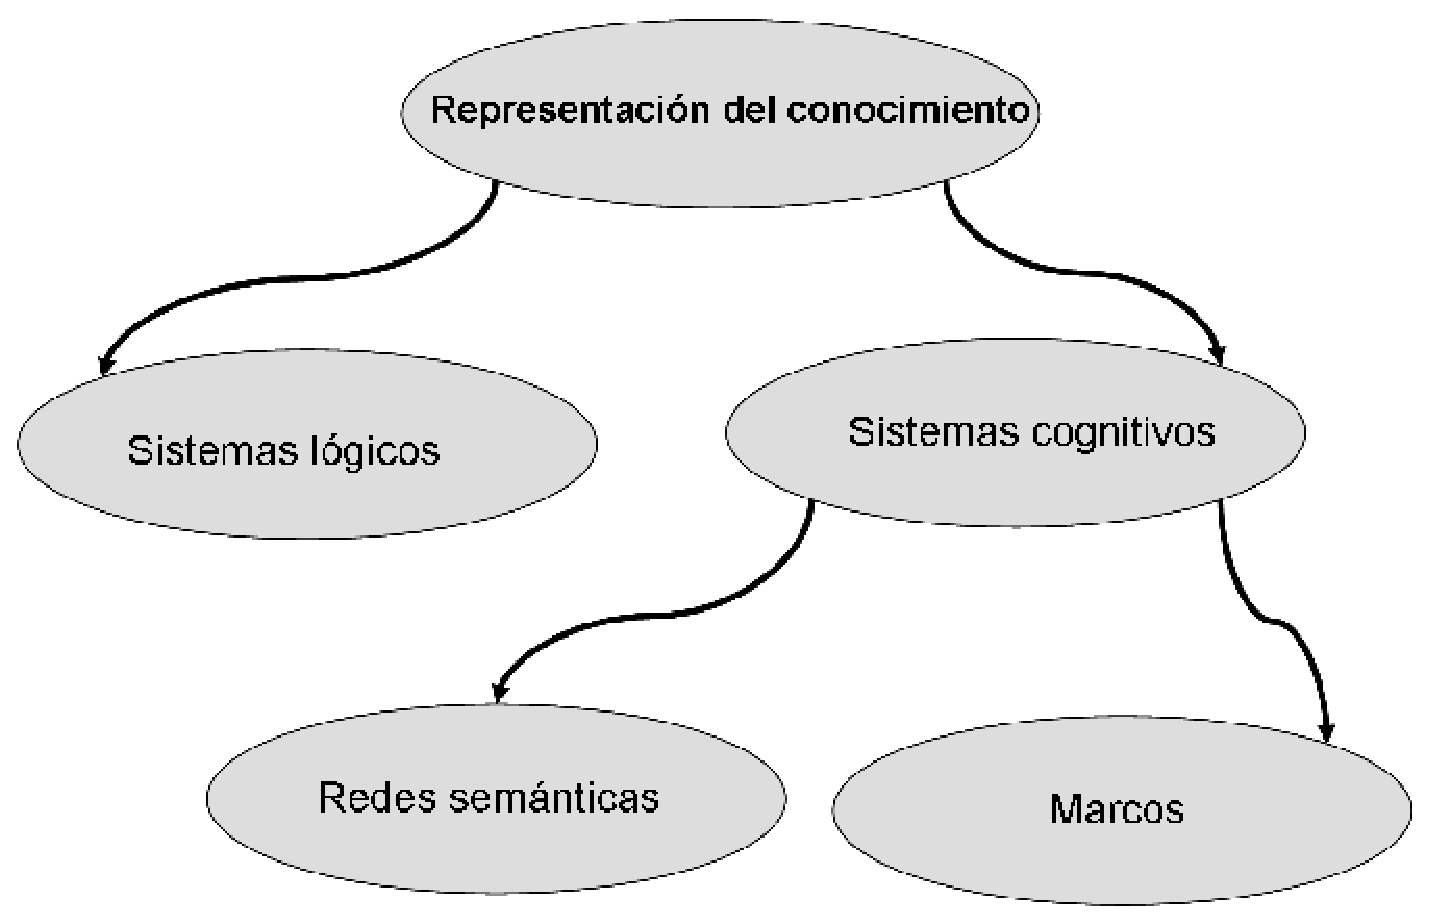
\includegraphics[width=10cm]{images/knowledge}
\caption{Sistemas basados en conocimiento.}
\label{fig:knowledge}
\end{figure}


\subsubsection{Clasificación de ontologías}
Las ontologías se pueden clasificar atendiendo a diferentes a criterios, a
continuación se exponen algunos de ellos.
\begin{description}
 \item [Grado de axiomatización.] Atendiendo a Sowa~\cite{Sowa99knowledge} las ontologías se pueden clasificar en:
\begin{description}
\item[Terminológicas:] define términos y sus relaciones en taxonomías que
involucran tanto relaciones de subtipo y supertipo, como las que relaciona
partes con un todo (\textit{part-whole}), no incluyen axiomas y definiciones
expresadas en lógica o lenguaje formal interpretable por una máquina. Por lo
tanto, existe menos información sobre el dominio modelado pero la simplicidad de
su especificación permite construir ontologías de gran tamaño.
\begin{example}
WordNet base de conocimiento (y datos) léxica.


Fuente: \url{http://wordnet.princeton.edu/}
\end{example}

\item[Formales:] consta de categorías restringidas por axiomas y definiciones
expresadas en alguna lógica formal, con menos conceptos pero preparadas para soportar
un procesamiento automático y servicios de razonamiento.

Una ontología terminológica podrá convertirse en formal a medida que se añadan
axiomas, aunque esta evolución no es ni mucho menos trivial.
\end{description}

\item[Según contexto.] Dependiendo del grado de dependencia del contexto las ontologías pueden ser:
\begin{description}
\item[Dominio:] modelan conceptualizaciones específicas, con restricciones de
estructura y contenido del dominio. Se reaprovecharán sólo en aquellas
aplicaciones que trabajen en ese dominio. Grado de dependencia alto.

\begin{example}
Ontología de medicina \textit{Galen}.


Fuente: \url{http://www.opengalen.org/}.
\end{example}

\item[Generales o de sentido común:] vocabularios o estructuras taxonómicas
genéricas. Alto grado de reaprovechamiento y bajo de dependencia del dominio.

\begin{example}
Cyc y OpenCyc.


Fuente: \url{http://www.cyc.com/}. 
\end{example}

\item[Metaontologías u ontologías genéricas:] ontologías de dominio genérico,
conceptos universales.
\begin{example}
DOLCE: Descriptive Ontology for Linguistic and Cognitive Engineering.


Fuente: \url{http://www.loa-cnr.it/DOLCE.html}. 
\end{example}

\end{description}

\item [Objeto de creación.]

Atendiendo al objetivo de creación de una ontología se establecen diferentes tipos:

\begin{itemize}
  \item Ontologías para la representación de conocimiento, como: \gls{OWL},
  \gls{DAML+OIL}, \gls{RDF}, RDF(S), OKBC, etc.
  \item Ontologías \textit{top level}, definen \textit{frameworks}, conceptos
  universales como las ya comentadas \textit{DOLCE} o \textit{Cyc}. 
  \item Ontologías para la definición de términos lingüisticos como
  \textit{WordNet} o \textit{EuroWordNet}~\cite{EuroWordNet}. 

	\item Ontologías de dominio, modelan conocimiento de cierto dominio: comercio
	electrónico o \textit{e-commerce}, de medicina \textit{Galen} o SNOMED, etc. 
\end{itemize}

\end{description}

Las ontologías como sistemas basados en conocimiento, serán más productivos
cuanto mejor ``informados'' estén, por ello, será interesante modelar utilizando
el mayor de grado de particularidad posible en el dominio, pero teniendo presente, que también es
importante mantener el objetivo de reutilizar conocimiento, podría ser interesante
enclavar los nuevos conceptos de dominio definidos dentro de las categorías de
alto nivel, para así alinear estas definiciones en un marco conceptual genérico.


\subsubsection{Principios de diseño}\label{onto-design}
Las ontologías deben o deberían cumplir una serie de principios:
\begin{description}
\item[Claridad:] proporcionar el significado pretendido a los términos
definidos. Definiciones tan objetivas como sea posible.
\item[Completitud:] las definiciones deberían recoger todas las condiciones
necesarias y suficientes, además de poseer una buena documentación en lenguaje natural.
 \item[Coherencia:] los términos definidos deben ser coherentes, concluyendo
 sólo aquellas inferencias consistentes con el modelo definido.
 \item[Extensibilidad:] anticipando la necesidad de reutilización y facilitando
 la adición de nuevo \linebreak conocimiento.
 \item[Mínimo compromiso ontológico:] minimizar el número de afirmaciones a
 realizar sobre el dominio modelado, permitiendo así que otros agentes las
 puedan refinar.

\item[Diversificación de jerarquías:] haciendo uso de la herencia múltiple, usar
tantos criterios de clasificación como sea posible. Así, añadir un nuevo concepto
es sencillo utilizando los ya existentes y la capacidad de clasificación.

\item[Minimizar la distancia semántica entre hermanos:] conceptos similares
deben agruparse.
 
  \item[Estandarización:] independencia simbólica, utilización de nombrado estándar.
 \item[Granularidad:] coherencia en el grado de particularidad, evitando el uso
 de términos ambig\"{u}os.
\end{description}

Finalmente, existen diversos procesos de desarrollo o metodologías que definen un
procedimiento para la captura de conocimiento de un dominio y la pertinente
construcción de ontologías. Por ejemplo: \textit{Methontology Framework} o \textit{Sensus method}. 


\subsubsection{Operaciones con ontologías}\label{op-ontologias}
En esta sección se describen las
operaciones~\cite{bruijn06-seman-web} que se pueden
realizar con las ontologías de acuerdo a su principio de reaprovechar el
conocimiento ya definido. La reutilización del conocimiento consensuado  es una de las
máximas de la creación de ontologías, para ello se definen tres operaciones
básicas (\textit{mapping} o correspondencia entre ontologías, \textit{merging} o
unión de ontologías y \textit{alignment} o descubrimiento de las
correspondencias de \textit{mapping} ) que
ayudan a la agregación de conocimiento basado en ontologías. La
importancia de estas operaciones se pone de manifiesto en la mediación de datos
entre fuentes heterogéneas, aspirando a resolver los conflictos que se producen
entre sistemas basados en conocimiento, que deben interaccionar entre sí pero que
han sido creados independientemente. El proceso de mediación, adquiere especial
interés para la propuesta de servicios web semánticos, en los cuales esta
operación es básica debido a la integración de ontologías provenientes de
diferentes modelos de negocio.  


\begin{description}
\item[\textit{Mapping} o \textit{mapeo} de ontologías:] especificación declarativa del
solapamiento semántico entre dos ontologías. Las correspondencias entre
entidades de ontologías diferentes son expresadas mediante axiomas en un
determinado lenguaje de \textit{mapeo}. Este proceso consta de tres fases: descubrimiento, representación y ejecución. Existen diferentes enfoques para llevar a cabo esta operación
como MAFRA, RDFT o C-OWL.
\item[\textit{Alignment} o alineamiento de ontologías:] proceso mediante el cual
se descubren las similitudes entre dos ontologías. El resultado es una especificación de los puntos en común, realizada a través del algoritmo 
\textit{Match operator}. Existen diferentes implementaciones como
Anchor-PROMPT, \linebreak GLUE, \textit{Semantic Matching} o QOM.
\item[\textit{Merging} o unión de ontologías:] creación de una ontología nueva
tomando como fuente dos o más ontologías. La nueva ontología unifica y reemplaza
las ontologías fuente. Se establecen dos enfoques para realizar esta
operación: 1) entrada de $n$ ontologías y salida de una sola
ontología, unión y reemplazo de las demás (por ejemplo: algoritmo
PROMPT~\cite{NM00}) y 2) entrada $n$ ontologías que no son reemplazadas, sino que se genera una ontología
\textit{bridge} que importa a las ontologías originales y especifica las correspondencias mediante
axiomas \textit{bridge}, por ejemplo \textit{OntoMerge}.
\end{description}

A la hora de afrontar la implementación de estas operaciones sobre ontologías se pueden generar dos tipos básicos de conflictos que impiden el éxito de la
operación y requieren intervención humana para facilitar la realización
automática de las operaciones: 
\begin{enumerate}
  \item Conflictos entre ``conceptualizaciones'' distintas del mismo dominio. A
  su vez, se distinguen dos categorías: 1) conflicto de ámbito, ocurre cuando dos clases tienen solapamiento en sus extensiones (el
  conjunto $s$ de instancias), y no coincide exactamente y 2) conflicto en la
  cobertura del modelo y su granularidad, ocurre si dos ontologías cubren parte
  de cierto dominio (por ejemplo: empleados de universidad y estudiantes) o bien
si una es más específica que otra (por ejemplo: una ontología define ``persona'' y otra define ``persona joven'').
  \item Conflictos entre las especificaciones de los conceptos. También, se diferencian tres categorías:\linebreak 1) conflicto en el estilo de
  modelado, cada ontología específica los conceptos de una manera determinada
(por ejemplo: tratamiento de las unidades de tiempo) o la descripción de los
conceptos   difiere (por ejemplo: utilización de subclases vs atributos); 2) conflicto
en la  terminología, dos conceptos son equivalentes pero no utilizan el mismo nombre,
  problema de sinónimos, o viceversa, son diferentes y utilizan el mismo nombre,
  homónimos y 3) conflicto de codificación, no se utilizan las mismas
  nomenclaturas, unidades de medida, etc.
\end{enumerate}

Todos estos conflictos, vienen en muchos casos provocados por no ajustarse a los
principios de diseño establecidos en la Sección~\ref{onto-design}. No
obstante, es habitual afrontar los problemas surgidos en la integración de ontologías ya que los
modeladores provienen de distintas partes, con diferente formación y puede que
sigan procedimientos particulares para la realización del modelado de
las ontologías, facilitando las tareas a las aplicaciones que las consuman.


\subsubsection{Aplicación de las ontologías}
Las ontologías se convierten en la pieza fundamental de ciertas áreas así pueden señalarse las 
siguientes:

\begin{description}
\item[Ingeniería del conocimiento:] las ontologías se pueden manifestar durante la ejecución de las siguientes tareas:
\begin{itemize}
  \item Construcción del modelo conceptual, generando los términos del glosario
  y de las relaciones que se establecen entre ellos.
  \item Construcción de la base de conocimiento, utilizando la ontología de
  modelado conceptual se pueden crear bases de conocimiento con la aplicación de
  reglas, restricciones, etc.
\end{itemize}

\item[Procesamiento del lenguaje natural:] mantenimiento de la definición de términos
gramaticales del lenguaje y las relaciones entre ellos.

\item[Integración de sistemas heterogéneos:] gestión de las diferencias
existentes entre diversos sistemas de información con el objetivo de facilitar
la comunicación entre los mismos.
\item[Búsqueda semántica:] utilizando conceptos y no términos para realizar las
búsquedas. 

\item[Web Semántica:] las ontologías son la base de la Web Semántica, por ello
cualquier aplicación que tenga un carácter semántico se apoyará, muy
probablemente, en ontologías.
\end{description}


Las ontologías se abren paso con fuerza sobre todo en el ámbito de las
aplicaciones~\cite{DBLP:conf/nldb/Penalver-MartinezVS11} de la Web Semántica, en particular en el escenario de la
integración de aplicaciones (servicios web semánticos~\cite{DBLP:journals/es/SanchezSMAVG11}) y contextualización del
usuario. En la construcción de una ontología, hay que afrontar el modelado desde el
punto de vista de la lógica (tipo y lenguaje de expresión) siguiendo los
principios de diseño, ver Sección~\ref{onto-design}, y no de la orientación a objetos, muy frecuente en el ámbito de la ingeniería del \textit{software}.  
   
\chapter{\label{capitulo:semantica}Panorámica de uso de la\\ Linked Data y Open Data} 
\section{\linkeddata}
En los últimos tiempos nos encontramos un entorno de datos fluyendo constantemente, esperando a ser utilizados para generar información
sobre un determinado acontecimiento. De esta manera, podemos ser conscientes de las últimas noticias, productos de una determinada
marca o simplemente sobre información de nuestros contactos en las redes sociales. Esta nueva situación implica que existe un nuevo
mercado para la construcción de aplicaciones y servicios~\cite{Krafzig2004} que exploten estos datos, generando nuevos negocios~\cite{web20} y conectando a las comunidades
científicas, y en general fomentando el progreso de una forma sostenible. Por ejemplo, algunos servicios de búsqueda como Google~\cite{Google} utilizan los
datos publicados en las tiendas de Internet como Amazon~\cite{Amazon}, para extender y procurar resultados de búsqueda más ajustados. En esta línea, prestando 
atención a los resultados de los principales buscadores, las primeras sugerencias corresponden a páginas de Wikipedia~\cite{Wikipedia}, Facebook~\cite{Facebook},
 Linkedin~\cite{Linkedin}, etc.,  por lo que efectivamente queda patente que los servicios de búsqueda~\cite{Pound}, entre otros, están sacando partido de los datos estructurados publicados en distintos sitios web, para así identificar descripciones, organizaciones, personas, perfiles profesionales o productos y 
ofrecer resultados más acordes con la intención de los usuarios.

La evolución hacia esta nueva web, también de denominada Web $3.0$, globalmente enlazada mediante datos supone una transición~\cite{Ankolekar07thetwo}
de la web tradicional orientada a documentos (Web $1.0$) y dirigida hacia las personas principalmente, incluyendo relaciones (Web $2.0$),
a una nueva \wod, en la cual los datos se publican para ser tratados por los humanos como
por los agentes automáticos, proporcionando descripciones más completas a todos los niveles. En este
sentido, Tim Berners-Lee explica convenientemente los principios de esta nueva web realizando una analogía 
de una bolsa de patatas~\cite{TBL-crisps} con una página web, en la cual la parte delantera estaría orientada 
hacia las personas, mientas que la información (meta información) de la parte trasera serían datos
dirigidos hacia otros agentes.

Actualmente la publicación de datos se haya envuelta en distintos dominios en los que previamente
nunca se había pensado compartir datos, pero en los cuales se están generando nuevos servicios y 
oportunidades de negocio a partir de esta iniciativa que busca la compartición de datos. En 
este estado pueden surgir varias preguntas:
\begin{itemize}
 \item ¿Cómo se deben publicar los datos para ser reutilizados?
\item ¿Existen mecanismos para la reutilización automática?
\item ¿Cuál es la forma más ágil para integrar fuentes de datos heterogéneas?
\item ¿Se puede asegurar la calidad de los datos en términos de disponibilidad, autenticidad, evolución, etc.?
\end{itemize}

Estamos, en consecuencia, ante una revolución del uso de datos en la Web, entorno en el cual se pueden realizar
diferentes operaciones sobre los mismos: descubrimiento, consulta, integración y explotación. La Web ofrece
su infraestructura~\cite{webarch}, protocolos y amplio asentamiento para reducir el impacto de esta evolución. No obstante, esta nuevo 
entorno trae consigo nuevos requisitos arquitectónicos, necesidad de entender el comportamiento de las \gls{URI}s~\cite{uri-rfc} y del 
protocolo \gls{HTTP}~\cite{http-rfc} para reutilizar la infraestructura existente y concienciar a la comunidad del empleo de este entorno. 

\subsection{Definición y necesidad de \textit{Linked Data}}\label{def-linkeddata}
Tim Berners-Lee acuñó esta iniciativa en el año 2006~\cite{Berners-Lee-2006} como parte de la Web Semántica~\cite{Berners-Lee2001,WeavingTim,berners-lee06a}. 
En un principio la Web Semántica surgió con el objetivo de integrar grandes bases de datos a través de modelos de conocimiento compartidos u ontologías, de esta manera
cualquiera podría reutilizar el conocimiento ya consensuado y en consecuencia los datos asociados a esta información. Si bien
la Web Semántica tuvo un gran éxito desde un punto de vista teórico, en la práctica escasas aplicaciones reales llegaron a tener
un notable impacto en el gran público~\cite{sw-use-cases}. Es por ello, que tomando la visión de la Web Semántica en su parte de modelos y formatos de datos
estandarizados formalizados a través de conocimiento compartido, fue tomada para definir lo que actualmente conocemos como \linkeddata~\cite{linked-data}.
En realidad se trata de un enfoque práctico de la Web Semántica, en el cual
se hace uso de los fundamentos de la semántica y de la web para proveer mecanismos para la publicación~\cite{bizer07how,Berr08} y 
consumo de datos masivos sin tener grandes barreras de entrada y claramente orientado al desarrollo de aplicaciones. 
Análogamente en el arranque de la web orientada a documentos se realizó un esfuerzo para la identificación sobre cómo publicar documentos, por ejemplo utilizando HTML, pero no se hizo hincapié en
modelar la información que se publicaba en los mismos, esto ocasionó que la Web que hoy conocemos despegara exponencialmente. En el caso
de la \wod se realiza un enfoque similar, es decir, se establece cómo publicar datos, sin embargo no realiza especial énfasis
 en que estos datos estén formalizados estrictamente sobre un modelo conocimiento. De esta manera se facilita y favorece el crecimiento y la aparición de nuevas fuentes
de datos en la Web. No obstante, esta segunda parte de modelado y estructuración de datos deviene fundamental para ciertas tareas
automáticas.

El objetivo por lo tanto de la \wod no se centra tan sólo en publicar datos sino en hacer los datos accesibles, tanto a las personas
como a las máquinas, como son actualmente los documentos disponibles en la Web. La diferencia sustancial reside en que actualmente
la web está orientada al uso por personas y las máquinas necesitan de procesos de un cierto grado de complejidad para acceder a esta información.
Por lo tanto, con esta nueva iniciativa se facilitan los enlaces entre los datos para que puedan ser explorados eficientemente 
por cualquier agente y realizar operaciones de enriquecimiento y enlazado de forma sencilla.

La \wod se construye sobre enlaces como la web tradicional en la que los documentos son enlazados entre sí. La diferencia
reside en que los datos utilizan enlaces en \gls{RDF} para describir recursos de distintos tipos identificados de forma unívoca
mediante un \gls{URI} y siguiendo unos principios que, aunque analizados en detalle en la Sección~\ref{principos-linked-data}, se presenta a continuación una breve descripción de los mismos:
\begin{itemize}
 \item \textit{Use URIs as names for things}. Utilizar URIs como nombres para identificar y acceder a los recursos.
 \item \textit{When someone looks up a URI, provide useful information, using the standards (RDF*, \gls{SPARQL}~\cite{Sparql})}. El acceso 
a los recursos a través de URIs debe estar basado en estándares como RDF o SPARQL suministrando igualmente información
sobre el acceso.
\item \textit{Include links to other URIs. so that they can discover more things}. Enlazar datos no sólo implica la publicación
masiva de datos sino que se deben establecer enlaces entre ellos con el objetivo de proveer un entorno navegable~\cite{Berners-lee06tabulator:exploring,Pietriga06fresnel}.
\item \textit{Use \gls{HTTP URI}s so that people can look up those names}. Utilizar URIs HTTP para reaprovechar la actual infraestructura
de la web y que el público potencial pueda acceder a los datos de la misma forma que hoy lo hace con los documentos.
\end{itemize}

En este contexto formalizado con reglas muy explícitas, queda patente 
que uno de los factores clave de esta iniciativa está en el poder de reutilizar información bien 
estructurada desde la propia fuente de datos, facilitando así la creación de aplicaciones fiables en el 
sentido del tratamiento de datos y evitando el uso de otras técnicas basadas en estadística y procesamiento
de lenguaje natural, que se siguen aplicando ya que no siempre se cumple con todos los requisitos que la iniciativa de \linkeddata establece.

En resumen, el objetivo de la iniciativa de \linkeddata es enlazar datos de fuentes heterogéneas entre sí, 
con el objetivo de enriquecer la información y ofrecer a todos los agentes tanto personas como máquinas
un espacio homogéneo basado en estándares para la realización de las operaciones citadas anteriormente, descubrimiento, acceso y explotación. 
Para ello se hace uso de la tecnología semántica \gls{RDF} que provee una forma flexible y escalable para la realización de descripciones de las entidades 
del mundo: personas, organizaciones, localizaciones, etc. Las sentencias en RDF permiten
establecer de una forma sencilla enlaces entre ellas creando conexiones desde un entorno local
hacia un entorno global. También cabe destacar que el uso de RDF difiere de los actuales
documentos presentes en la web en dos puntos importantes:

\begin{itemize}
 \item El enlace se produce a nivel de entidades, no de documentos.
 \item Cada enlace tiene un tipo definido.
\end{itemize}

\linkeddata permite así establecer conexiones entre diferentes fuentes de datos y crear un espacio 
de datos global, esto es posible gracias al uso de estándares y de un modelo de datos común que facilita
la creación de aplicaciones de carácter general capaces de operar en este nuevo espacio de datos.

El gran valor de \linkeddata se centra por tanto en brindar una oportunidad para utilizar los datos
y explotar su valor mediante sistemas basados en conocimiento, con capacidad de procesar una cantidad
masiva de datos obteniendo así soluciones más fiables y aproximadas a las necesidades y expectativas
de los agentes. En síntesis, ver Tabla~\ref{tabla:linked-data}, se pueden establecer una serie de características y criterios a satisfacer.
\begin{longtable}[c]{|l|p{7cm}|p{8cm}|} 
\hline
  \textbf{ID} & \textbf{Directriz} &  \textbf{Descripción} \\\hline
\endhead
   \multicolumn{3}{|c|}{\textbf{Principios Linked Data}}  \\ \hline
   1.1&\textit{Use URIs as names for things} & \\ \hline
   1.2&\textit{When someone looks up a URI, provide useful information, using the standards (RDF*, SPARQL)} & \\ \hline  
   1.3&\textit{Include links to other URIs} & \\ \hline    
   1.4&\textit{Use HTTP URIs} & \\ \hline    
  \multicolumn{3}{|c|}{\textbf{Modelo $\star$}}  \\ \hline
     2.1&$\star$	& \textit{Available on the web (whatever format) but with an open licence, to be \opendata} \\ \hline 

2.2&$\star \star$	 &  \textit{Available as machine-readable structured data (e.g. excel instead of image scan of a table)} \\ \hline 

2.3&$\star \star \star$	&  \textit{ as (2) plus non-proprietary format (e.g. \gls{CSV} instead of exce}l) \\ \hline 

2.4&$\star \star \star \star$	&  \textit{All the above plus, Use open standards from \gls{W3C} (RDF and SPARQL) to identify things, so that people can point at your stuff} \\ \hline 
 
2.5&$\star \star \star \star \star$	 & \textit{All the above, plus: Link your data to other people’s data to provide context}                                     \\ \hline 
  \hline
  \caption{Características a tener en cuenta sobre \linkeddata.}
  \label{tabla:linked-data}
\end{longtable}

\subsection{\opendata}\label{opendata-sect}
Este término se enclava dentro de las definiciones de conocimiento abierto realizadas por
la organización \textit{Open Knowledge Foundation}~\cite{okfn} (\gls{OKFN}), en el cual también se incluyen:
\begin{itemize}
 \item Contenidos como libros, películas, música y cualquier otro material con autoría definida.
\item Datos, en general, pertenecientes a distintos contextos: científicos, históricos o geográficos.
\item Información proveniente de las Administraciones Públicas.
\end{itemize}

Siguiendo la definición realizada por esta institución, cuando una obra o datos satisfagan las siguientes
condiciones serán consideradas como abiertas:

\begin{description}
 \item [Acceso.] La obra debe estar disponible íntegramente y sólo a un coste de 
  reproducción razonable, preferiblemente para su descarga de modo gratuito en Internet. 
  La obra también debe estar disponible en una forma conveniente para ejecutar modificaciones sobre ella.
 \item [Redistribución.] La licencia no debe contener restricciones sobre la posibilidad de venta o 
  distribución de la obra en sí misma o formando parte de un paquete constituido por obras de fuentes diversas. 
  La licencia no debe exigir un pago u otro tipo de cuota para esta venta o distribución.
 \item [Reutilización.] La licencia debe permitir hacer modificaciones y obras derivadas facultando que éstas sean distribuidas en las mismas condiciones que la obra original. La licencia puede imponer algún tipo de requisito relativo al 
  reconocimiento y a la integridad: veáse el principio 5 (Reconocimiento) y el principio 6 (Integridad) reseñados más adelante.
 \item [Ausencia de restricciones tecnológicas.] Se debe proporcionar la obra de modo que no presente ningún obstáculo tecnológico para ejecutar los actos mencionados anteriormente. Esto se puede conseguir ofreciendo la obra en un formato de datos abierto, por ejemplo un formato cuya especificación esté disponible públicamente y de manera gratuita y que para su uso no se imponga ninguna restricción de tipo monetario o análogas.
 \item [Reconocimiento.] La licencia puede exigir como condición para la redistribución y la reutilización el reconocimiento de los contribuyentes y creadores de la obra. Si se impone esta condición, no debe ser de manera onerosa. Por ejemplo si se exige un reconocimiento, la obra debería ir acompañada de una lista de aquellos que hay reconocer.
 \item [Sin discriminación de personas o grupos.] La licencia no debe discriminar a ninguna persona o grupo de personas.
 \item [Sin discriminación de ámbitos de trabajo.] La licencia no debe contener restricciones sobre el uso en un ámbito de trabajo específico. Por ejemplo, no se puede limitar el uso de la obra en un negocio, o que ésta sea utilizada para investigación militar.
 \item [Distribución de la licencia.] Los derechos adjuntos a la obra deben aplicarse también a todo áquel a quien le sea redistribuida, sin necesidad de que éste disponga una licencia adicional.
 \item [La licencia no debe ser específica de un paquete.] Los derechos adjuntos a la obra no deben depender de que la obra forme parte de un paquete particular. Si la obra se extrae de ese paquete y se utiliza o se distribuye en las condiciones de la licencia de la obra, todos aquellos a quien les sea redistribuida deberán tener los mismos derechos que los concedidos conjuntamente con el paquete original.
 \item [La licencia no debe restringir la distribución de otras obras.] La licencia no debe imponer restricciones en otras obras distribuidas conjuntamente con la obra objeto de la licencia. Por ejemplo, la licencia no debe imponer que todas las otras obras que se distribuyan por el mismo medio sean abiertas.
\end{description}

La corriente de datos abiertos~\cite{odfn} ha sido especialmente acogida en el ámbito de las Administraciones
Públicas, ver Figura~\ref{fig:od-spain}, adaptando las directrices aquí fijadas para desplegar el movimiento
de \ogd. 

\begin{figure}[!htb]
\centering
	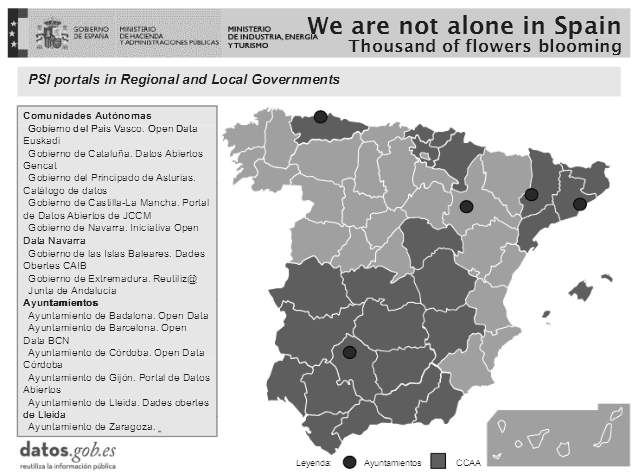
\includegraphics[width=14cm]{images/phd/open-data-spain}
\caption{Estado de \opendata en España}
\label{fig:od-spain}
\end{figure}

Las instituciones públicas han establecido distintos canales de comunicación~\cite{improvingW3c}
con los ciudadanos, intentando siempre mejorar la interacción en los distintos
procesos administrativos. Por ello y para estar presentes en las principales iniciativas
de comunicación han procurado atender a los avances tecnológicos. Desde
principios de la década de los años 90 han tenido presencia en la web proveyendo
distintos servicios para que el ciudadano pueda agilizar sus trámites
y así obtener una administración más eficiente, tanto en tiempo como en uso
de recursos. Esta situación ha derivado a lo que se denomina como ``administración
electrónica'' o \egov, en la cual la información de los servicios
y datos que obran en poder de la Administración resultan de fácil acceso a los
 ciudadanos a través de los principales canales de comunicación, 
como la web, dispositivos móviles, etc., creando de esta forma
una administración con una ventanilla única, fijando como objetivo principal
 la transparencia y la objetividad, materializadas a través de distintas
políticas, concretamente en el caso europeo se dispone de un Plan de Acción~\cite{policy-eu} específico para el período 2011-2015.

No obstante, aunque las intenciones están acertadamente fijadas existen muchos
desafíos que han estado y están impidiendo el despegue definitivo de la administración
electrónica, desde la tecnología hasta el necesario cambio tanto para los
integrantes de la propia administración como para los ciudadanos. Proveer
servicios y datos a través de la red se ha convertido en un desafío en el cual
las distintas administraciones se encuentran inmersas, esta situación
implica ejecutar una gran inversión para dar cabida a todas las necesidades desde un punto
de vista tanto en materia de infraestructura como de concienciación social. De esta forma,
un gobierno basado en administración electrónica debe ser capaz de fijar los requisitos
de los servicios y datos a liberar, asegurar la autenticidad y definir la legislación
pertinente que establezca un marco jurídico seguro para que los ciudadanos pueden utilizar
toda la información disponible para consultar o construir nuevos servicios de valor
añadido sobre ellos.

Entre las actividades que se presentan como claves para el desarrollo de la administración
electrónica se pueden referir los siguientes:
\begin{itemize}
 \item Uso y aplicación de estándares.
 \item Transparencia y participación.
 \item Concienciación de los avances en la gestión e integración de datos.
 \item Relaciones y colaboraciones.
\end{itemize}

En este contexto se determinan por una parte los objetivos de la administración
respecto a disponer un entorno flexible y dinámico para sus ciudadanos, y por otra parte 
se encuentra el comportamiento de las propias personas y organizaciones. Actualmente
se advierte un entorno definido por las siguientes características: 
global, conectado, cambiante y accesible en su mayor parte.

El término de \ogd ha sido designado en la administración de Estados Unidos para indicar
aquellos datos o registros de información que obran en poder de la Administración Pública y que
han sido recabados con distintos objetivos en los distintos procesos administrativos. Como ejemplos
de reutilización en el sector público encontramos los siguientes dominios: salud, cartografía, datos
meteorológicos, educación, datos bibliográficos, contratación pública, legislación, etc. Como 
se ha comentado con carácter previo, las organizaciones públicas producen, almacenan y distribuyen distintos tipos
de información: legal, financiera, geográfica, etc., en su actividad diaria. Esta información
proveniente del sector público (\gls{PSI}) está enclavada dentro de un marco jurídico, por ejemplo en Europa la Directiva 2003/98/EC~\cite{d2003,d2003-update},
 que puede variar de un país a otro, en España la Ley 37/2007~\cite{l37-2007} y su Real Decreto 1495/2011~\cite{r-1495} 
de desarrollo, Reino Unido~\cite{uk2012}, Francia~\cite{fr2012} o la iniciativa de la Casa Blanca en Estados Unidos~\cite{usa}. 
Habitualmente se utilizaban distintas técnicas y formatos
para la distribución de la información del sector público por diferentes canales desde el papel y correo postal, hasta
formatos electrónicos y las propias páginas web. La evolución en los últimos
años ha sido de gran calado de modo que ha hecho necesario dictar una legislación común que 
debe ser transpuesta en los diferentes países, como ocurre en el caso de Europa.

La transición hacia este nuevo enfoque administrativo todavía se encuentra
en una etapa temprana debido a las dificultades que supone toda una nueva forma de
actuar. En general, se suele hablar de \gd y \pusi para referirse al mismo concepto. Se han realizado diferentes definiciones como las
presentes en la iniciativa \ogd, pero no sólo se trata de exponer de forma pública 
las grandes bases de datos gubernamentales, sino que éstos deberían cumplir 
unos principios~\cite{8-principles} que a continuación se listan:

\begin{enumerate}
 \item Data Must Be \textit{Complete}. \textit{All public data are made available. Data are electronically stored information or recordings, including but not limited to documents, databases, transcripts, and audio/visual recordings. Public data are data that are not subject to valid privacy, security or privilege limitations, as governed by other statutes.}
 \item Data Must Be \textit{Primary}. \textit{Data are published as collected at the source, with the finest possible level of granularity, not in aggregate or modified forms.}
 \item Data Must Be \textit{Timely}. \textit{Data are made available as quickly as necessary to preserve the value of the data.}
 \item Data Must Be \textit{Accessible}. \textit{Data are available to the widest range of users for the widest range of purposes.}
 \item Data Must Be \textit{Machine processable}. \textit{Data are reasonably structured to allow automated processing of it.}
 \item Access Must Be \textit{Non-Discriminatory}. \textit{Data are available to anyone, with no requirement of registration.}
 \item Data Formats Must Be \textit{Non-Proprietary}. \textit{Data are available in a format over which no entity has exclusive control.}
 \item Data Must Be \textit{License-free}. \textit{Data are not subject to any copyright, patent, trademark or trade secret regulation. Reasonable privacy, security and privilege restrictions may be allowed as governed by other statutes.}
\end{enumerate}

Con todo ello, se provee un entorno en el cual ``público'' designa a las condiciones que deben cumplir los datos
para considerarse ``abiertos'', no se entra a valorar los datos que se deben liberar ni tampoco cuestiones
legales. En cuanto a los ``datos'', se toma este término para designar a los registro electrónicos, es importante
destacar que los documentos físicos no se consideran como tal, que obran en poder de la administración y finalmente,
con ``revisable'' se denomina a aquellos datos para los cuales existe una persona de contacto que actúa como
enlace para aquellos que quieran usar los datos, para gestionar el uso de los mismos y para los cuales
existe un organismo administrativo o judicial que posee la potestad para aplicar los principios antes
citados adecuadamente.

Por otra parte, existen cuestiones~\cite{publishing-ogd} que deben tener respuesta en el contexto de \ogd desde un punto
de vista estratégico hasta funcional como qué tipo de interfaz de acceso (\gls{API}) se debe proveer para el acceso a los datos, por ejemplo, 
en cuanto a los datos a liberar, la iniciativa de datos abiertos no especifica qué datos deberían liberarse. Corresponde
a la estrategia del organismo en cuestión establecer las prioridades, coste y beneficios de la liberación de un determinado conjunto
de datos. En determinados casos como el del Gobierno de Reino Unido~\cite{uk-survey} o el Ayuntamiento de Zaragoza~\cite{zar-survey} se utilizan encuestas
a los propios usuarios para especificar o establecer un orden en los datos a liberar. El objetivo final será
disponer de una política y guías de apertura de datos que sean capaces de dar soporte a los siguientes puntos:

\begin{description}
 \item [Inclusión.] El uso de estándares facilita la accesibilidad y la usabilidad de los datos. De esta forma,
se facilita la participación de terceros y el desarrollo de aplicaciones de distinto carácter que beneficiarán
transversalmente a toda la sociedad con nuevos servicios.
\item [Transparencia.] En los últimos años y debido a los múltiples casos de corrupción a nivel político, deficiente gestión
de fondos públicos y en general, cierta falta de claridad por parte de las instituciones ha hecho que esta corriente
se sitúe como un eje el impulso de la transparencia en el conjunto de las administraciones públicas.
\item [Responsabilidad.] La eficiencia en el uso de recursos debe ser uno de los objetivos de la administración pública, por ello
conseguir información sobre cómo funciona la administración puede permitir mejorar su funcionamiento interno.
\end{description}

Una vez que se dispone de datos abiertos cabe definir cómo se pueden obtener mejoras en ciertos procesos de uso. Entre 
ellos se puede destacar:

\begin{description}
\item [Reutilizar.] La información abierta permite plantear nuevos modelos de interacción, tanto para otras administraciones públicas
como para organizaciones o comunidades que se beneficien de estos datos para el despliegue de nuevos servicios~\cite{web20}. Actualmente
se realizan actividades para el impulso de la reutilización de datos, como los concursos en los que se liberan datos a los que interesados
presentan aplicaciones haciendo uso de ellos.
 \item [Generar múltiples vistas de los datos~\cite{DBLP:journals/semweb/DadzieR11}.] Cuando se dispone de los datos de una forma más o menos estandarizada y con facilidad
de acceso se pueden generar múltiples vistas, dependiendo de las necesidades del usuario y adaptándolos al contexto. Por ejemplo,
generación de informes en PDF, visualización en mapas de la información geográfica, etc. Partiendo de los mismos datos y en algunos
casos y tras la ejecución de un proceso de enriquecimiento se puede mejorar la información que provee. El coste de realización de 
estos procesos es alto si está centralizado en la administración, pero se puede diversificar y abaratar delegando en 
terceras partes.
 \item [Mejorar los actuales sistemas de búsqueda~\cite{hoga-etal-2011-swse-JWS}.] Un sistema de búsqueda dispondrá de mayor precisión cuanto más ``informado'' esté, por lo tanto,
si se pueden reutilizar los datos ya disponibles para mejorar los resultados de las consultas de los usuarios, se facilitará el acceso a la
información.
  \item [Integrar fuentes de datos~\cite{Andreas_Schultz_Isele_Bizer_Becker_2011,Harth:2011:SIP:1963192.1963318}.] Habitualmente cada organismo goza de cierta independencia para gestionar sus propios datos. La realidad
es que en muchos casos diferentes organismos de la misma entidad tienen la necesidad de cruzar datos para obtener diferente información
agregada. Si se utilizan datos abiertos se favorece la integración y la reutilización de datos disminuyendo los costes de la obtención
y gestión de los mismos al no estar multiplicada.
\end{description}

Una vez que se han definido algunos de los beneficios del uso de datos abiertos en el ámbito de las
administraciones públicas, cabe ahora especificar cómo han de ser publicados para que
puedan ser consumidos por terceros de forma ágil. Para ello se han establecido una serie
de directrices o métodos:
\begin{itemize}
 \item Usar anotaciones basadas en microformatos o \gls{RDFa}~\cite{rdfa-primer} en \gls{XHTML} o \gls{HTML}5~\cite{HTML5}.
 \item Facilitar la accesibilidad siguiendo las directrices \gls{WCAG}~\cite{wcag2}.
 \item Desplegar APIs específicas para el consumo de datos.
 \item Sindicar de contenidos mediante \gls{RSS}~\cite{rss} o \gls{ATOM}~\cite{atom-rfc}.
 \item Proveer interfaces \gls{REST}~\cite{Fielding2000} o \gls{SOAP}~\cite{SOAP11} de servicios de acceso a datos.
 \item Aplicar tecnologías semánticas mediante \gls{RDF}.
\end{itemize}

Finalmente se ha de definir la misión y estrategia de apertura de datos, así la confianza (\trust), procedencia~\cite{Carroll05namedgraphs,prov-group} (\provenance) y calidad de los mismos, la
evolución en tiempo, las limitaciones tecnológicas y la capacidad para seguir creciendo. De acuerdo a lo expuesto en esta sección se pueden
establecer una serie de factores a evaluar sobre la publicación de datos abiertos de acuerdo a distintos criterios y que 
servirán para evaluar si se cumplen las guías definidas. 

\subsection{\lod}
La convergencia entre las iniciativas de \linkeddata y \opendata ha conllevado la creación
de un nuevo término para designar a aquellos datos que cumplen las guías de ambas iniciativas y que 
se denomina \lod. Bajo esta definición se agrupan todos los datos que han sido
liberados aplicando los principios de \linkeddata y que además cumplen significativamente
las directrices de \opendata. Habitualmente este término se aplica en el contexto de las Administraciones
Públicas, en las que el esfuerzo por la apertura de datos ha sido intenso y en el que han logrado grandes avances. 

El alto valor de los datos enlazados abiertos permite disfrutar a terceros de la posibilidad real 
de creación de servicios de alto valor añadido. No obstante, surge la duda de si el proceso de enlazado de datos
y de explotación, corresponde a la propia Administración o si cabe delegar el mismo. En este sentido, existen
una serie de cuestiones que se han de plantear:
\begin{description}
 \item [¿Debe la Administración explotar los datos y construir aplicaciones para su consumo?] En un primer momento, las Administraciones
Públicas cubrían toda la cadena valor de uso de los datos, desde su apertura hasta su explotación. En estos momentos, se está produciendo
un cambio de dirección en cuestiones de sostenibilidad que implica que la creación de servicios y aplicaciones se delega en terceros. Si bien
como punto de partida es conveniente que la Administración demuestre el valor del uso de los datos, una vez que se ha producido
la sensibilización necesaria resulta evidente que deben ser terceras partes quienes reutilicen los datos.
\item [¿Qué nivel de \linkeddata debe proveer la Administración?] El caso ideal sería que los datos liberados se encontrarán
en el estatus de 5 $\star$ pero la realidad es que tanto por parte de la comunidad de desarrolladores, habituados
a tecnologías como \gls{RSS} o APIs \gls{REST}, como por el propio coste
que genera llegar a este nivel, en muchos casos no es realmente útil realizar este esfuerzo, con la simple apertura de datos
y un modelo de acceso convenientemente homogéneo es suficiente.
\item [¿Sobre la calidad de los datos?] Como se ha comentado es fundamental para motivar la creación de aplicaciones
la confianza en los datos que se están utilizando. En este sentido poder verificar su procedencia, evolución en el tiempo, autenticidad
y en general, su nivel de confianza y calidad es vital para el triunfo de esta corriente en aplicaciones de alto valor añadido. El esfuerzo
de la Administración debe centrarse por consiguiente en este punto, asegurando a la comunidad la confianza en los datos
que van a usar.
\item [¿Qué estructura se debe seguir en los organismos públicos para liberar los datos?] Existen principalmente dos enfoques
para abordar la apertura de datos masiva: \textit{top-down} y \textit{bottom-up}. El enfoque \textit{top-down} se está
utilizando en el Gobierno de Reino Unido y consiste básicamente en fijar las directrices, modelos, etc., que se han de seguir para liberar
datos desde un organismo central que propaga esta metodología a todos los sectores y organismos públicos que deseen abrir sus datos. Por el contrario,
el enfoque \textit{bottom-up} tiene su paradigma en la Administración española en el cual han surgido numerosos conjuntos de datos aplicando
sus propias directrices. Determinar cuál es el mejor modelo depende del nivel de precisión que se establezca en cuanto a la publicación de datos, en contraposición
con el coste del mismo y el tiempo empleado. El enfoque \textit{top-down} si bien es más homogéneo, requiere un enérgico esfuerzo común inicial tanto en tiempo
como en coste, pero en el largo plazo es más sostenible puesto que todos los organismos reaprovechan la experiencia. En cambio, el enfoque \textit{bottom-up} permite
un despliegue inicial más rápido multiplicando el esfuerzo y los costes en cada organismo candidato a la apertura de datos, pero 
con la posibilidad de que uno de los modelos particulares se convierta en referente.
\item [¿Cómo se debe prevenir la privacidad de los datos?] Si bien por la propia definición de datos enlazados abiertos no se debiera tener
en cuenta esta cuestión, si que surge la necesidad en contextos determinados ofrecer mecanismos de control para prevenir el uso inadecuado
de datos, por ejemplo los denominados ``secretos estadísticos'' y así evitar infringir otras leyes como las referidas a datos personales.
\item [¿Puede la Administración establecer un modelo de negocio, ver Figura~\ref{fig:data-business-model}, sobre los datos?] Este punto genera cierta controversia, ya que el coste de posesión 
de los datos recae sobre los ciudadanos, actualmente cualquier servicio público o proceso administrativo tiene unos costes que se financian
a través de determinadas tasas. En el caso de la apertura de datos se considera que no debe suponer un coste adicional para los administrados
pero la realidad es que el coste implícito está presente, es más, algunos organismo utilizan este mecanismo como medio de auto-financiación. Desde un punto
de vista de los agentes implicados, los terceros que utilicen estos datos no estarán dispuestos a pagar un sobrecoste por su uso, la propia Administración
no estaría incentivada a la aplicación de tasas sobre estos datos presumiendo que el retorno provisto de terceros sea capaz de financiar la apertura de los datos. Reiterando que 
por definición los datos deberían ser libres también es necesario la creación de un entorno sostenible y probablemente el enfoque óptimo en el 
estadio inicial sea de conformidad a un modelo libre.
\item [Otras cuestiones.] Relacionadas con los datos a liberar, realimentación de los mismos (\textit{crowdsourcing}) para corregir errores, reconciliación, etc. siguen todavía abiertas y obtendrán respuesta paulatinamente, en función la propia demanda.
\end{description}

\begin{figure}[!htb]
\centering
	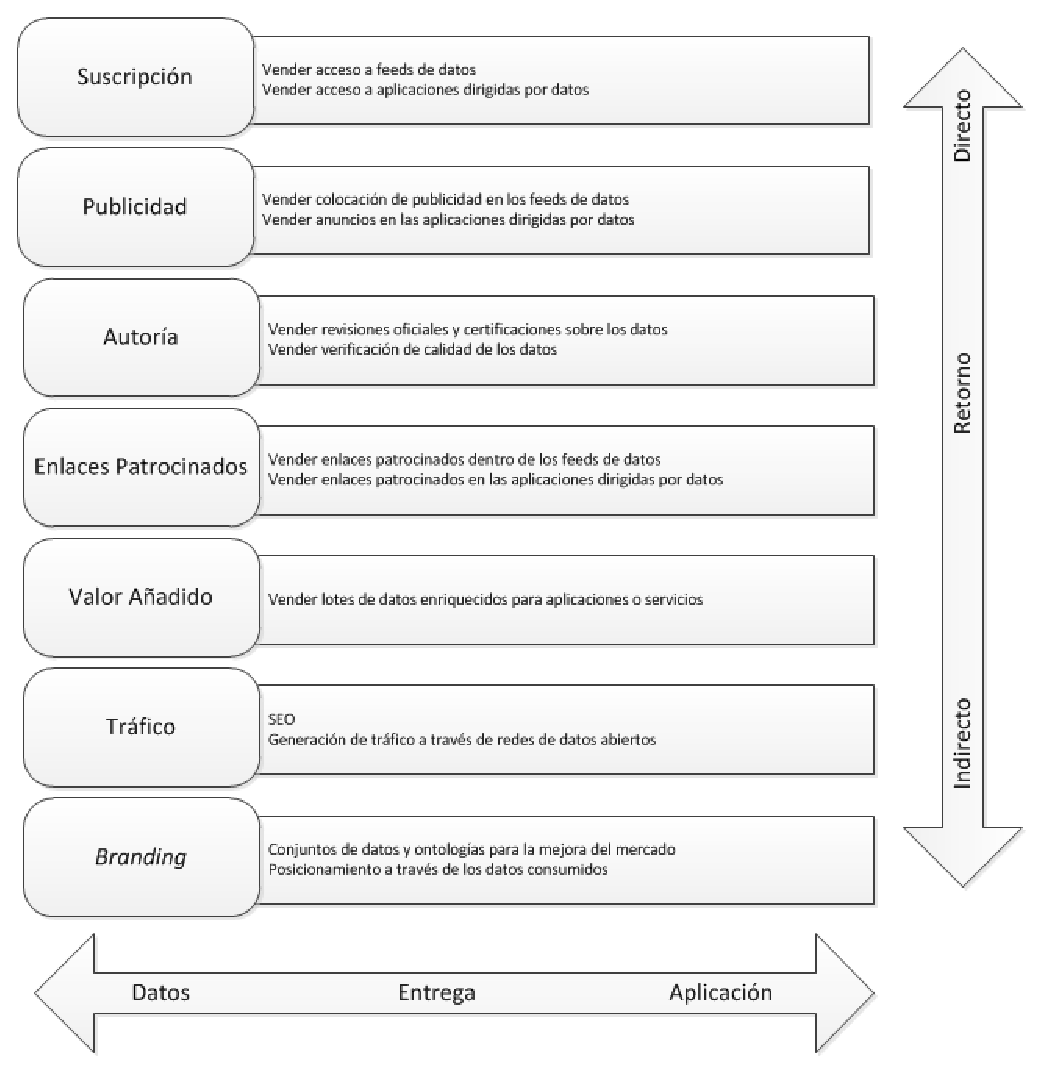
\includegraphics[width=12cm]{images/phd/data-business-models}
\caption{Modelos de negocio para datos (extraída de \textit{Chief Marketing Technologist}).}
\label{fig:data-business-model}
\end{figure}


En definitiva, la conjunción de los principios de \linkeddata y \opendata ha conllevado una corriente de actuación
en las Administraciones Públicas con amplios beneficios tanto para los ciudadanos como para las empresas. La experiencia inicial es altamente
enriquecedora para las partes implicadas y su tendencia es seguir creciendo. No obstante, también se presentan varias cuestiones
abiertas que se habrán de ir resolviendo a la vez que la tecnología y la experiencia se incrementan.
\subsection{Principios de \linkeddata}\label{principos-linked-data}
En las secciones anteriores se han repasado las líneas que marcan la definición de \linkeddata, se pueden resumir
en una corriente que aúna la tecnología semántica más madura con la apertura de datos, en un infraestructura perfectamente
establecida como es la Web.

Los principios de \linkeddata~\cite{Berners-Lee-2006} se reducen a los siguientes cuatro puntos:

\begin{itemize}
 \item \textit{Use \gls{URI}s as names for things}. La utilización de URIs como nombres para identificar y acceder a los recursos. Este principio busca el uso de URIs como camino para referenciar de forma única a todos
los recursos disponibles, no sólo documentos, así: contenidos digitales, vídeos, sensores~\cite{ontology-search,Jeung:2010:EMM:1850003.1850235}, 
  organizaciones~\cite{open-corporates}, personas~\cite{facebook-ld}, etc., con el objetivo de ampliar el contexto de un espacio virtual a uno real.
 \item \textit{When someone looks up a URI, provide useful information, using the standards (RDF*, SPARQL~\cite{Sparql})}. El acceso 
a los recursos a través de URIs debe estar basado en estándares como \gls{RDF} o \gls{SPARQL} proveyendo igualmente información
sobre cómo acceder.
\item \textit{Include links to other URIs. so that they can discover more things}. El enlazado de datos no sólo implica la publicación
masiva de los mismos, sino que se deben establecer enlaces entre ellos con el objetivo de proveer un entorno 
navegable~\cite{Berners-lee06tabulator:exploring,Pietriga06fresnel} y de consulta~\cite{Hartig09executingsparql}.
\item \textit{Use \gls{HTTP URI}s so that people can look up those names}. La utilización de URIs HTTP para reaprovechar la actual infraestructura
de la web y que el público potencial pueda acceder a los datos de la misma forma que se realiza actualmente con los documentos.
\end{itemize}

En general estos principios buscan una manera estándar de identificar, modelar, acceder y consumir recursos para que la creación
de aplicaciones y servicio sea lo más sencilla y ágil posible.

Por lo tanto, para atender a estos principios se deben facilitar una serie de mecanismos que permitan:
\begin{itemize}
 \item Nombrar a todas las cosas, recursos, etc., mediante URIs.
 \item Referenciar y acceder a los contenidos mediante URIs. Uso de \textit{hash}, \textit{slash} URIs o código $303$ de \gls{HTTP}. 
 \item Proveer información útil sobre los recursos de forma estándar mediante RDF. Uso de literales o de enlaces a otras
descripciones RDF. Negociación de contenido.
 \item Incluir enlaces a otros datos. Podemos establecer tres tipos de enlaces principales: relación, identidad y 
vocabulario. Cada uno permite establecer relaciones, alinear unos recursos con otros y definir las descripciones
respectivamente.
\end{itemize}

Los beneficios de la utilización de estos mecanismos que sustentan a los $4$ principios citados proporcionan las siguientes ventajas:
\begin{itemize}
 \item Escala global. El uso de \gls{RDF} permite unificar la información de los recursos, modelo, formato y acceso a los datos.
 \item Enlace entre recursos. RDF da soporte a la reutilización intrínseca de recursos ya definidos dando cabida
a la unión de datos de diferentes fuentes.
  \item Expresividad. La información en RDF se puede representar combinando distintos vocabularios.
 \item Estructuración. Utilizando un modelo definido en RDF(S) u \gls{OWL} se da soporte al modelo de los datos
mediante mecanismos estándar, compartidos y reutilizables.
\end{itemize}

Además de estas ventajas, existen ciertas características que deberían evitarse, tales como los mecanismos
de reificación de RDF, las colecciones o el uso de nodos en blanco con el objetivo de facilitar la consulta
mediante el lenguaje SPARQL. En cuanto a los formatos en los que se pueden presentar los datos enlazados en RDF se encuentra:
\gls{RDFa}~\cite{rdfa-primer}, \gls{RDF/XML}~\cite{rdf-syntax}, \gls{Turtle}~\cite{turtle-syntax}, \gls{N3}~\cite{n3-syntax} ,\gls{RDF}/\gls{JSON}~\cite{rdf-binario} o RDF binario~\cite{rdf-json}.


En definitiva, se trata de proveer un entorno estándar y global de datos en el cual se utilice un modelo
de datos estandarizado y único (RDF), con capacidad para enlazar a otros datos y que todos ellos se auto-describan
en el sentido de facilitar a sus descripciones beneficiando el descubrimiento, acceso e integración de datos.

\subsection{Construyendo una nueva \wod}
Este nuevo entorno de publicación de datos ha implicado que numerosas personas y organizaciones
se hayan inclinado por la aplicación de los principios de los datos enlazados en la apertura de sus datos. Como resultado
se puede establecer que el despegue de la \wod es ya un hecho, creando un grafo global de billones
de tripletas RDF de diferentes tipos y fuentes enlazadas~\cite{HoganUHCPD:2012:237} entre sí. En general, esta eclosión se debe
a varias razones: genericidad, estandarización, dominio público, capacidad de representación de la información, expresividad,
reutilización de tecnología estable, etc. Como origen de este enfoque se puede situar la iniciativa
del \lod~\cite{lod-group} (\gls{LOD}) del W3C en el año 2007, en el cual se sentaron las bases de la actual \wod, dando comienzo el desarrollo tecnológico así como la transformación de los primeros conjuntos de datos. Entre ellos
podemos destacar el esfuerzo de la DBPedia~\cite{dbpedia2009} o herramientas como \gls{Pubby}, D2RServer, etc. La evolución
de la \wod queda recogida en el diagrama de la nube de \datasets (\textit{LOD Cloud}~\cite{linked-data-cloud}) que en su última
versión recoge hasta 320 \datasets, ver Figura~\ref{fig:lod-cloud}, y continua en aumento si se consulta \textit{The Data Hub}~\cite{the-data-hub}. A modo informativo a fecha de septiembre
de 2010 en el diagrama anteriormente citado estaban disponibles unos 203 \textit{datasets} (en diciembre
de 2011 llegan hasta 326), más de 25 billones de tripletas \gls{RDF} y unos 395 millones de enlaces entre los diferentes datos.

\begin{figure}[!htb]
\centering
	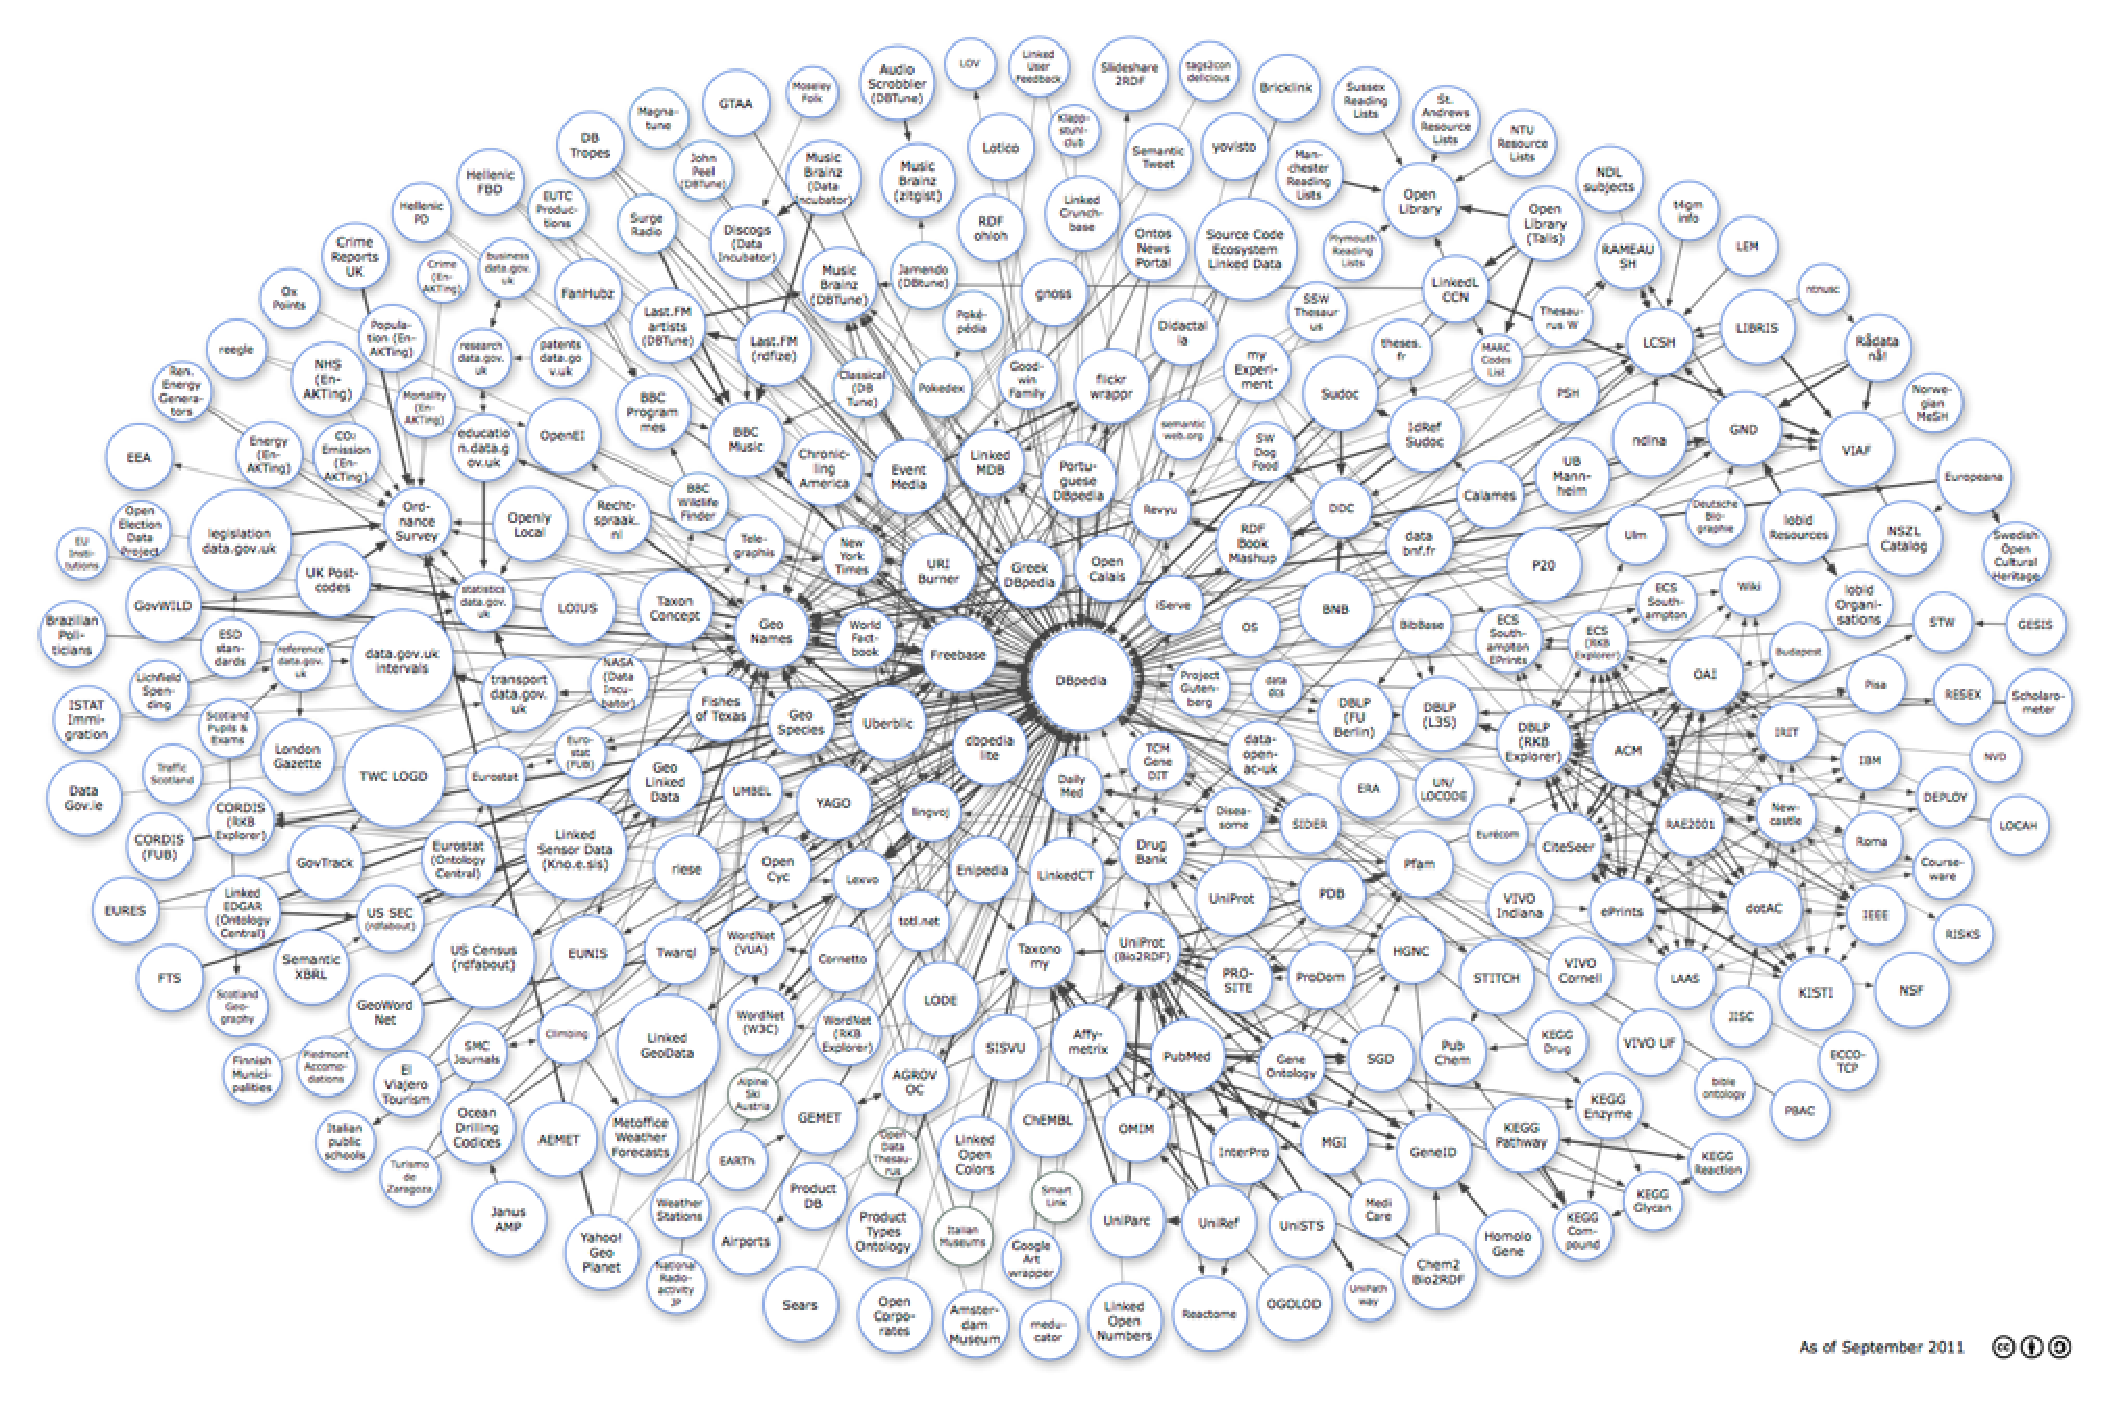
\includegraphics[width=10cm]{images/phd/lod-datasets_2011-09-19_1000px}
\caption{\textit{Linking Open Data cloud diagram, by Richard Cyganiak and Anja Jentzsch}.}
\label{fig:lod-cloud}
\end{figure}

Por otra parte, la información que se puede encontrar en la nueva \wod es tan variada como en la actual
web de documentos, a continuación algunos de los ejemplos de los datos que podemos encontrar, así:

\begin{itemize}
 \item Genéricos o de carácter transversal, candidatos ser reutilizados por cualquier conjunto de datos: DBPedia~\cite{Bizer:2009:D-C:1640541.1640848}, 
Freebase~\cite{freebase}, etc.
 \item Geográficos: Geonames~\cite{geonames}, OpenStreetMap~\cite{open-street-maps} o GeoLinkedData~\cite{SLHA11}.
 \item ``Government Data'': Data Gov UK, Datos.es, etc.
 \item Educación, Multimedia, Bibliográficos, Científicos, Médicos, ``Social Media'', etc., que se pueden encontrar clasificados
en la versión del diagrama de la nube de \lod bajo diferentes colores.
\end{itemize}

A la hora de unirse a la \wod hay que tener en cuenta varias consideraciones, además de proveer
datos enlazados se deben tener en cuenta unos principios relativos al diseño:

\begin{description}
 \item [Diseño de las \gls{URI}s.] Se busca que las URIs referencien a objetos reales y que se puedan obtener
descripciones a través de los protocolos propios de Internet, alineado directamente con el segundo principio de datos
enlazados y en este sentido hay que tener en cuenta varios aspectos: 
\begin{itemize}
 \item Uso de ``minting \gls{HTTP URI}s'': son URIs que están bajo el control del aquel que publica datos, es decir, utiliza
las URIs de su dominio para los datos y documentos.
\item ``Cool URIs''~\cite{Sauermann+2007a,bernerslee1998uri}: las URIs deben permanecer en el tiempo, en todo caso los usuarios las pueden cambiar, pero los identificadores
deberían permanecer inalterados. De la misma forma, se debe proveer un mecanismo para que a través de una misma URI se pueda
acceder a distinto contenido mediante negociación de contenido, extensiones, etc. 
\item ``Meaningful URIs'' vs ``ID based URIs''~\cite{uris-uk}: al igual que en el punto anterior nos encontramos ante la tesitura
de diseñar identificadores que se puedan recordar y con significado respecto a su contenido o bien utilizar
identificadores autogenerados. En cualquier caso, la decisión dependerá de la información a identificar, pero 
hay que tener presente este factor como clave en el diseño de la identificación de datos.
\end{itemize}
\item [Descripción de recursos con \gls{RDF}.] En este sentido se han establecido una serie de buenas prácticas y patrones
para describir los datos de los recursos susceptibles de publicación, ver Sección~\ref{metodologias}. Es importante seguir estas guías con el objeto de facilitar
su consulta a través de lenguajes como \gls{SPARQL}.
\item [Metainformación sobre los datos publicados.] No se trata sólo de publicar datos, ni de la apertura de las bases de datos
a la web, sino también de suministrar información sobre qué, cómo y dónde se puede acceder a estos datos. Para ello,
se debe atender a los siguientes criterios:
\begin{itemize}
 \item Usar vocabularios para describir el \dataset como \gls{voID}~\cite{void} o ``Semantic Sitemaps''\cite{Cyganiak08semanticsitemaps}.
 \item Añadir información sobre la procedencia~\cite{DBLP:conf/ipaw/HartigZ10,w3c-prov} de los datos (\provenance).
 \item Añadir información sobre la licencia~\cite{ld-licencias} de uso de los datos y los derechos de autoría, copia, distribución y modificación.
 \item Añadir información sobre la evolución temporal~\cite{ld-memento}, se puede conseguir mediante diferentes técnicas, incluyendo
la información en las URIs, en las descripciones RDF o mediante negociación de contenido.
\end{itemize}

\item [Seleccionar vocabularios a utilizar.] Existe un gran número de vocabularios~\cite{dcat-group} diseñados para describir
diversos tipos de información. La tendencia es reutilizar los vocabularios existentes~\cite{lod-stats} en la medida de lo posible, 
evitando re-modelar información ya descrita. Aunque existen catálogos de vocabularios, finalmente es la experiencia
y la consulta de otros \datasets la principal vía de información para seleccionar los vocabularios a reutilizar.
En general se atenderá a los siguientes factores: uso actual, mantenimiento, cobertura y expresividad.

\item [Enlazar con otros ``\datasets''.] Al igual que en el punto anterior no existe una forma estándar
de realizar este proceso, puede ser manual o automático, pero si que es necesario fijar la atención en la semántica del enlace y seleccionar aquellos recursos que sean
de mayor uso para asegurar de nuevo la coherencia de nuestros datos y su difusión.

\item [Publicar los datos.] Una vez determinados los datos a publicar, los cuales se han transformado y enlazado (si resultara oportuno), es
necesario proceder a su publicación de forma estandarizada mediante la aplicación de ciertos patrones definidos y teniendo en cuenta
si los datos son o no dinámicos, la criticidad, el esfuerzo de duplicar bases de datos, los formatos que van a ser soportados,
la exposición mediante servicios de consulta, el uso de un API, etc.
\item [Consumir datos publicados.] Este proceso conlleva la explotación de los datos disponibles tanto para generar
nuevos servicios de negocio comerciales o simplemente para consultar la información que se haya publicada y que se 
puede enriquecer con el universo de los demás \textit{datasets} publicados.
\item [Difundir los datos publicados.] Aunque no se trata de una acción o requisito funcional, el éxito de un conjunto
de datos publicados dependerá en buena medida, además de su calidad~\cite{ld-quality} y facilidad de acceso, de la difusión que se realice
sobre su uso y capacidad. Para ello, existen diversos catálogos~\cite{TummarelloDO07} y herramientas de indexado, por ejemplo
\textit{thedatahub.org}, \textit{prefix.cc}, etc., en los cuales se puede incluir los datos publicados para que así, terceros 
los puedan consumir. La información de difusión deberá incluir aspectos relativos sobre cómo acceder a los datos, qué datos están publicados, el tipo de licencia, etc., para asegurar la confianza necesaria en los usuarios finales.

\end{description}

Como se ha reseñado en los puntos anteriores, pese a que existen patrones, recetas y métodos de producción, publicación y consumo de datos
es decisión del responsable la selección de los mismos. Si bien la flexibilidad de actuación queda patente y beneficia
la publicación masiva de datos, lleva consigo una desventaja, que reside en la posibilidad de errar en ciertos puntos provocando
una baja calidad en los datos. Para ello, tal y como se expone en la siguiente sección existen diversos esfuerzos para poner en común
estas guías bajo una metodología especificando las actividades, participantes, herramientas y productos de entrada y salida
en cada una de las partes del proceso. En nuestro caso, esta situación es de especial relevancia para poder evaluar las ventajas
de uso de datos enlazados, en contraposición con la actual situación de manejo de datos en el campo de la contratación pública
electrónica.

\subsection{Metodologías y Buenas Prácticas}\label{metodologias}
En las anteriores secciones se han presentando las diferentes iniciativas entorno a datos enlazados en un contexto
general, pero teniendo presentes las necesidades de la administración pública electrónica. Han quedado patentes las necesidades,
ventajas y algunas desventajas del uso de esta iniciativa para los procesos de producción, publicación y consumo de datos. Si 
bien existen muchas guías y principios de diseño que se pueden extraer a través de la literatura, es conveniente repasar
los enfoques que se están desarrollando para realizar una guía sobre cómo se deben aplicar los conceptos de  \linkeddata, \opendata, \ogd, \lod, etc., 
para ello existen diferentes guías e incluso plataformas que aglutinan una serie de características de interés que a continuación se listan, 
repasando las más destacadas.

\begin{itemize}
 \item \textit{Linked Data Design Considerations} del libro \textit{Linked Data: Evolving the Web into a Global Data Space}~\cite{Heath_Bizer_2011}.
 \item \textit{Linked Data Patterns}~\cite{linked-data-patterns}.
 \item \textit{Best Practices}~\cite{best-gld,Berr08} del grupo de trabajo del \gls{W3C} \textit{Government Linked Data First \gls{F2F} June 29-30, 2011}~\cite{gld-group}.
 \item \textit{Linked Data Cookbook}~\cite{linked-data-cookbook} del grupo de trabajo del W3C \textit{Government Linked Data Working Group}~\cite{gld-group}.
 \item \textit{Government Linked Data-Life Cycle}~\cite{gld-lifecycle} del grupo de trabajo del W3C \textit{Government Linked Data Working Group}.
 \item \textit{Publishing Open Government Data}~\cite{publishing-ogd} borrador de trabajo del W3C.
 \item \textit{LOD2 Stack}~\cite{lod2-stack} del proyecto europeo \textit{LOD2}~\cite{lod2-project}.
 \item \textit{Toward a Basic Profile for Linked Data}~\cite{basic-profile-w3c,basic-profile-ibm} de IBM.
 \item Metodología~\cite{DBLP:conf/i-semantics/Cifuentes-SilvaSG11,methodologyCaepia2011} propuesta por la Universidad de Oviedo en el ámbito de la Biblioteca del Congreso de Chile.
 \item \textit{Talis Platform}~\cite{talis}.  
 \item \textit{Linked Open Data: The Essentials}~\cite{Bauer2012}.
\item Documentación específica de cada país e incluso región para el despliegue de \opendata.
\end{itemize}

El objetivo de estas guías es definir unas directrices sobre cómo publicar los datos para obtener una \wod de calidad. Además y en 
esta misma línea se están organizando continuamente conferencias, talleres, etc., específicos dentro de los grandes eventos científicos
para divulgar las actividades relacionadas con \linkeddata, como por ejemplo \textit{Consuming Linking Open Data}~\cite{cold} (\gls{COLD}), 
\textit{Linked Data On the Web}~\cite{ldow} (\gls{LDOW}), \textit{Social Data On the Web}~\cite{sdow} (\gls{SDOW}) o \textit{Linked Enterprise Data Patterns}~\cite{linked-enterprise-data-patterns} que sirven 
como concentrador de las actividades que se están realizando en este ámbito y que abordan los principales problemas 
que aparecen en este entorno emergente.

\subsubsection{\textit{Linked Data Design Considerations}}\label{linked-data-design-issues}
En el libro~\cite{Heath_Bizer_2011} realizado por Chris Bizer (investigador en la Freie Universitat de Berlin, Alemania y creador de la DBPedia) y 
por Tom Heath (uno de los investigadores principales de la plataforma Talis~\cite{talis}) se ponen de manifiesto una serie de consideraciones, ver Tabla~\ref{table:linkeddata-design-book}
de diseño a tener en cuenta cuando se pretende desplegar una plataforma de datos enlazados. 


\begin{longtable}[c]{|l|p{7cm}|p{8cm}|} 

\hline

  \textbf{ID} & \textbf{Directriz} &  \textbf{Descripción} \\\hline

\endhead
   1& \multicolumn{2}{|c|}{\textbf{\textit{Using URIs as Names for Things}}}\\ \hline
   1.1 &  \textit{Minting \gls{HTTP URI}s} & Las URIs deben permitir acceder a los recursos que nombran. Uso del schema HTTP. \\ \hline
   1.2 &  \textit{Use of Cool URIs} &  Las URIs deben seguir unos criterios de diseño que permitan y animen a terceros su uso.\\ \hline
   1.3 &  \textit{Keep out of namespaces you do not control} &  Las URIs de los recursos deben pertenecer a un dominio sobre el que se tenga control.\\ \hline
   1.4 &  \textit{Abstract away from implementation details} & Las URIs no incluyen detalles de implementación como el formato del recurso. \\ \hline
   1.5 &  \textit{Use Natural Keys within URIs} &  Para asegurar que las URIs son únicas se utiliza una clave primaria o ID para identificar recursos.\\ \hline
   1.6 &  \textit{Hash URIs} &  La concatenación de identificadores en el URI se realiza utilizando \# como separador final del recurso.\\ \hline
   1.7 &  \textit{Slash URIs} &  Igual que en el caso anterior pero utilizando $/$. \\ \hline
   2&\multicolumn{2}{|c|}{\textbf{\textit{Describing Things with RDF}}}\\ \hline
   2.1 &  \textit{\gls{RDF} resources} & Cuando se accede a un recurso a través de un \gls{URI} se debe proveer información útil. \\ \hline
   2.2 &  \textit{Literal Triples and Outgoing Links} & El sujeto de la información en RDF es siempre el URI del recurso que se está describiendo. \\ \hline
   2.3 &  \textit{Incoming Links} & Proveer enlaces a otros recursos para hacer los datos navegables. \\ \hline
   2.4 &  \textit{Triples that Describe Related Resources} & Describir parcialmente los recursos que son enlazados desde el actual. \\ \hline
   2.5 &  \textit{Triples that Describe the Description} & Añadir metainformación sobre los propios recursos como licencia. \\ \hline
  3&\multicolumn{2}{|c|}{\textbf{\textit{Publishing Data about Data}}}\\ \hline
   3.1 &  \textit{Describing a Data Set} & Añadir metainformación sobre el conjunto de datos que se está publicando. \\ \hline
   3.2 &  \textit{Use of Semantic Sitemaps} & Utilizar la extensión de \textit{Sitemap} para describir los datos proveyendo capacidades nuevas para los buscadores. \\ \hline
   3.3 &  \textit{Use of voiD Descriptions} & Utilizar el vocabulario voiD (the Vocabulary of Interlinked Datasets) para la metainformación de los datos. Es considerado el estándar de facto. \\ \hline
   3.4 &  \textit{Provenance Metadata} & Añadir información sobre la procedencia de los datos. Capacidades de monitorización y evolución en el tiempo. \\ \hline
   3.5 &  \textit{Licenses, Waivers and Norms for Data} & Incluir información sobre el uso posible de los datos a través de una licencia. \\ \hline
   3.6 &  \textit{Non-copyrightable Material} & $\approxeq$ \\ \hline
   4&\multicolumn{2}{|c|}{\textbf{\textit{Choosing and Using Vocabularies to Describe Data}}}\\ \hline
   4.1 &  \textit{\gls{SKOS}, RDFS and \gls{OWL}} &  Modelar la información de los datos de acuerdo a un vocabulario estándar. Proveer un modelo formal para los datos.\\ \hline
   4.2 &  \textit{Annotations in RDFS} &  Usar las anotaciones \texttt{rdfs:label} y \texttt{rdfs:comment} en las descripciones de RDF.\\ \hline
   4.3 &  \textit{Relating Classes and Properties} &  Relacionar los recursos en RDF mediante propiedades de RDFS, SKOS, etc.: \texttt{rdfs:subClassOf}, \texttt{skos:related}, etc.  \\ \hline
   4.4 &  \textit{Reusing Existing Terms} & Reutilizar las definiciones ya concebidas en los vocabularios existentes de los distintos dominios como: Dublin Core, FOAF, etc. \\ \hline
   4.5 &  \textit{Selecting Vocabularies} & Seleccionar los vocabularios a reutilizar teniendo en cuenta: \textit{Usage and uptake}, \textit{Maintenance and governance}, \textit{Coverage} y \textit{Expressivity}.\\ \hline
   4.6 &  \textit{Defining Terms} &  Si los vocabularios existentes no cubren las necesidades de nuestros datos, definir nuevos términos.\\ \hline
   5&\multicolumn{2}{|c|}{\textbf{\textit{Making Links with RDF}}}\\ \hline
   5.1 &  \textit{Publishing Incoming and Outgoing Links} &  Publicar un volcado de los datos en RDF.\\ \hline
   5.2 &  \textit{Making Links with External Data Sources} &  Reutilizar y enriquecer las descripciones en RDF con otras ya existentes asegurando que existen.\\ \hline
   5.3 &  \textit{Choosing External Linking Targets} & Los enlaces a datos externos deben cumplir que sean referenciables mediante un URI y deberían ser reutilizados por otros.\\ \hline
   5.4 &  \textit{Choosing Predicates for Linking} & Similar al punto $22$.\\ \hline
   5.5 &  \textit{Setting RDF Links Manually} & Incluir enlaces en las descripciones en RDF mediante edición manual (si de forma automática no es fiable).\\ \hline
   5.6 &  \textit{Auto-generating RDF Links} & Incluir enlaces las descripciones en RDF de forma automática. Uso de herramientas de reconciliación de entidades: SILK, LIMES, etc.\\ \hline
   5.7 &  \textit{Key-based Approaches} & Los enlaces se realizan mediante búsqueda de recursos con palabras claves.\\ \hline
   5.8 &  \textit{Similarity-based Approaches} & Los enlaces se realizan mediante búsqueda de recursos de acuerdo a una estructura.\\ \hline
  6&\multicolumn{2}{|c|}{\textbf{\textit{Recipes for Publishing Linked Data}}}\\ \hline
   6.1 &  \textit{Linked Data Publishing Patterns} & Establecer el modelo para ofrecer los datos.\\ \hline
   6.2 &  \textit{From Queryable Structured Data to Linked Data} & Exportar una base de datos relacional mediante un mapeador a RDF.\\ \hline
   6.3 &  \textit{From Static Structured Data to Linked Data} & Transformar datos estáticos a RDF. Por ejemplo: CSV, MSExcel, etc.\\ \hline
   6.4 &  \textit{From Text Documents to Linked Data} & Extraer los datos RDF de documentos de texto.\\ \hline
   6.5 &  \textit{Data Volume: How much data needs to be served?} & Dependiendo de la cantidad de datos definir qué datos y cantidad se pueden exportar.\\ \hline
   6.6 &  \textit{Data Dynamism: How often does the data change?} & Dependiendo de los cambios en los datos definir qué patrón (\textit{from}) se adapta mejor a la exportación de los datos.\\ \hline
   6.7 &  \textit{Serving Linked Data as Static RDF/XML Files} & Publicar los ficheros en RDF en un servidor web. Forma más sencilla.\\ \hline
   6.8 &  \textit{Hosting and Naming Static RDF Files} & Utilizar una convención de nombrado y negociación de contenido para los ficheros en RDF. Reglas de reescritura en servidor web.\\ \hline
   6.9 &  \textit{Server-Side Configuration: \gls{MIME} Types} & Servir el contenido apropiado de acuerdo a los tipos MIME.\\ \hline
   6.10 &  \textit{Making RDF Discoverable from \gls{HTML}} & Permitir que desde HTML se pueda reutilizar las descripciones en RDF.\\ \hline
   6.11 &  \textit{Serving Linked Data as RDF Embedded in HTML Files} & Enriquecer HTML con las descripciones en RDF. Por ejemplo con RDFa.\\ \hline
   6.12 &  \textit{Serving RDF and HTML with Custom Server-Side Scripts} & Generación bajo demanda de RDF en el servidor.\\ \hline
   6.13 &  \textit{Serving Linked Data from Relational Databases} & Generación bajo demanda de RDF en el servidor mapeando a una base de datos.\\ \hline
   6.14 &  \textit{Serving Linked Data from RDF Triple Stores} & Utilizar las capacidades de un triple-store para ofrecer RDF.\\ \hline
   6.15 &  \textit{Serving Linked Data by Wrapping Existing Application or Web \gls{API}s} & Exportar los datos de las aplicaciones web existentes como RDF.\\ \hline
   6.16 &  \textit{Testing and Debugging Linked Data} & Utilizar herramientas para verificar que se cumple con los principios de \linkeddata y de la publicación de datos.\\ \hline
   7&\multicolumn{2}{|c|}{\textbf{\textit{Architecture of Linked Data Applications}}}\\ \hline
   7.1 &  \textit{The Crawling Pattern} & Se navega por los recursos RDF con el objeto de extraer los datos para proveer servicios y datos a una capa superior.\\ \hline
   7.2 &  \textit{The On-The-Fly Dereferencing Pattern} & El patrón de los navegadores de \linkeddata que extraen la información de los recursos en el momento en el que se necesita.\\ \hline
   7.3 &  \textit{The Query Federation Pattern} & Se crean consultas complejas ejecutadas sobre varias fuentes de datos que se presentan al usuario dentro de una aplicación.\\ \hline
 
\hline
\caption{Consideraciones de Diseño \linkeddata}\label{table:linkeddata-design-book}\\    
\end{longtable}

Como se puede comprobar, en esta lista residen una serie de consideraciones a valorar en relación con la producción, publicación y consumo de datos
enlazados. La implementación o el uso que se realice de cada uno de estos puntos depende de la estrategia seguida por la persona o institución
implicada en el proceso de ofrecer sus datos bajo la iniciativa \linkeddata. Finalmente y tras aplicar estos principios se puede utilizar
el siguiente \textit{checklist}, es similar al utilizado para añadir un conjunto de datos a la iniciativa \gls{LOD} Cloud,
 para verificar, ver Tabla~\ref{table:linkeddata-check-list}, si se han 
aplicado de forma correcta los principios de diseño propuestos por los autores y en consecuencia de \linkeddata.


\begin{longtable}[c]{|l|p{7cm}|p{8cm}|} 

\hline

  \textbf{ID} & \textbf{Punto a cumplir} &  \textbf{Descripción} \\\hline

\endhead
   1 &  \textit{Does your data set links to other data sets?} & Existen enlaces externos desde las descripciones en RDF a otros externos que conformen un grafo global .\\ \hline
   2 &  \textit{Do you provide provenance metadata?} &  Los datos disponen de información sobre su procedencia.\\ \hline
   3 &  \textit{Do you provide licensing metadata?} &  Se establecen las restricciones necesarias sobre el uso de los datos.\\ \hline
   4 &  \textit{Do you use terms from widely deployed vocabularies?} & Las descripciones en \gls{RDF} se basan en reutilizar clases y propiedades ya existentes y aplicadas ampliamente. \\ \hline
   5 &  \textit{Are the URIs of proprietary vocabulary terms dereferenceable?} & Las clases y propiedades definidas particularmente son referenciables. \\ \hline
   6 &  \textit{Do you map proprietary vocabulary terms to other vocabularies?} &  Las clases y propiedades definidas se basan y relacionan con otras ya existentes y aplicadas ampliamente.\\ \hline
   7 &  \textit{Do you provide data set-level metadata?} &  Se ofrece metainformación sobre el conjunto de datos en general\\ \hline
   8 &  \textit{Do you refer to additional access methods?} &  Además del uso de \gls{URI}s para referenciar los datos se proveen otros servicios como un \textit{endpoint} de SPARQL.\\ \hline

\hline
\caption{\textit{Checklist} \linkeddata}\label{table:linkeddata-check-list}\\    
\end{longtable}

\begin{figure}[!htb]
\centering
	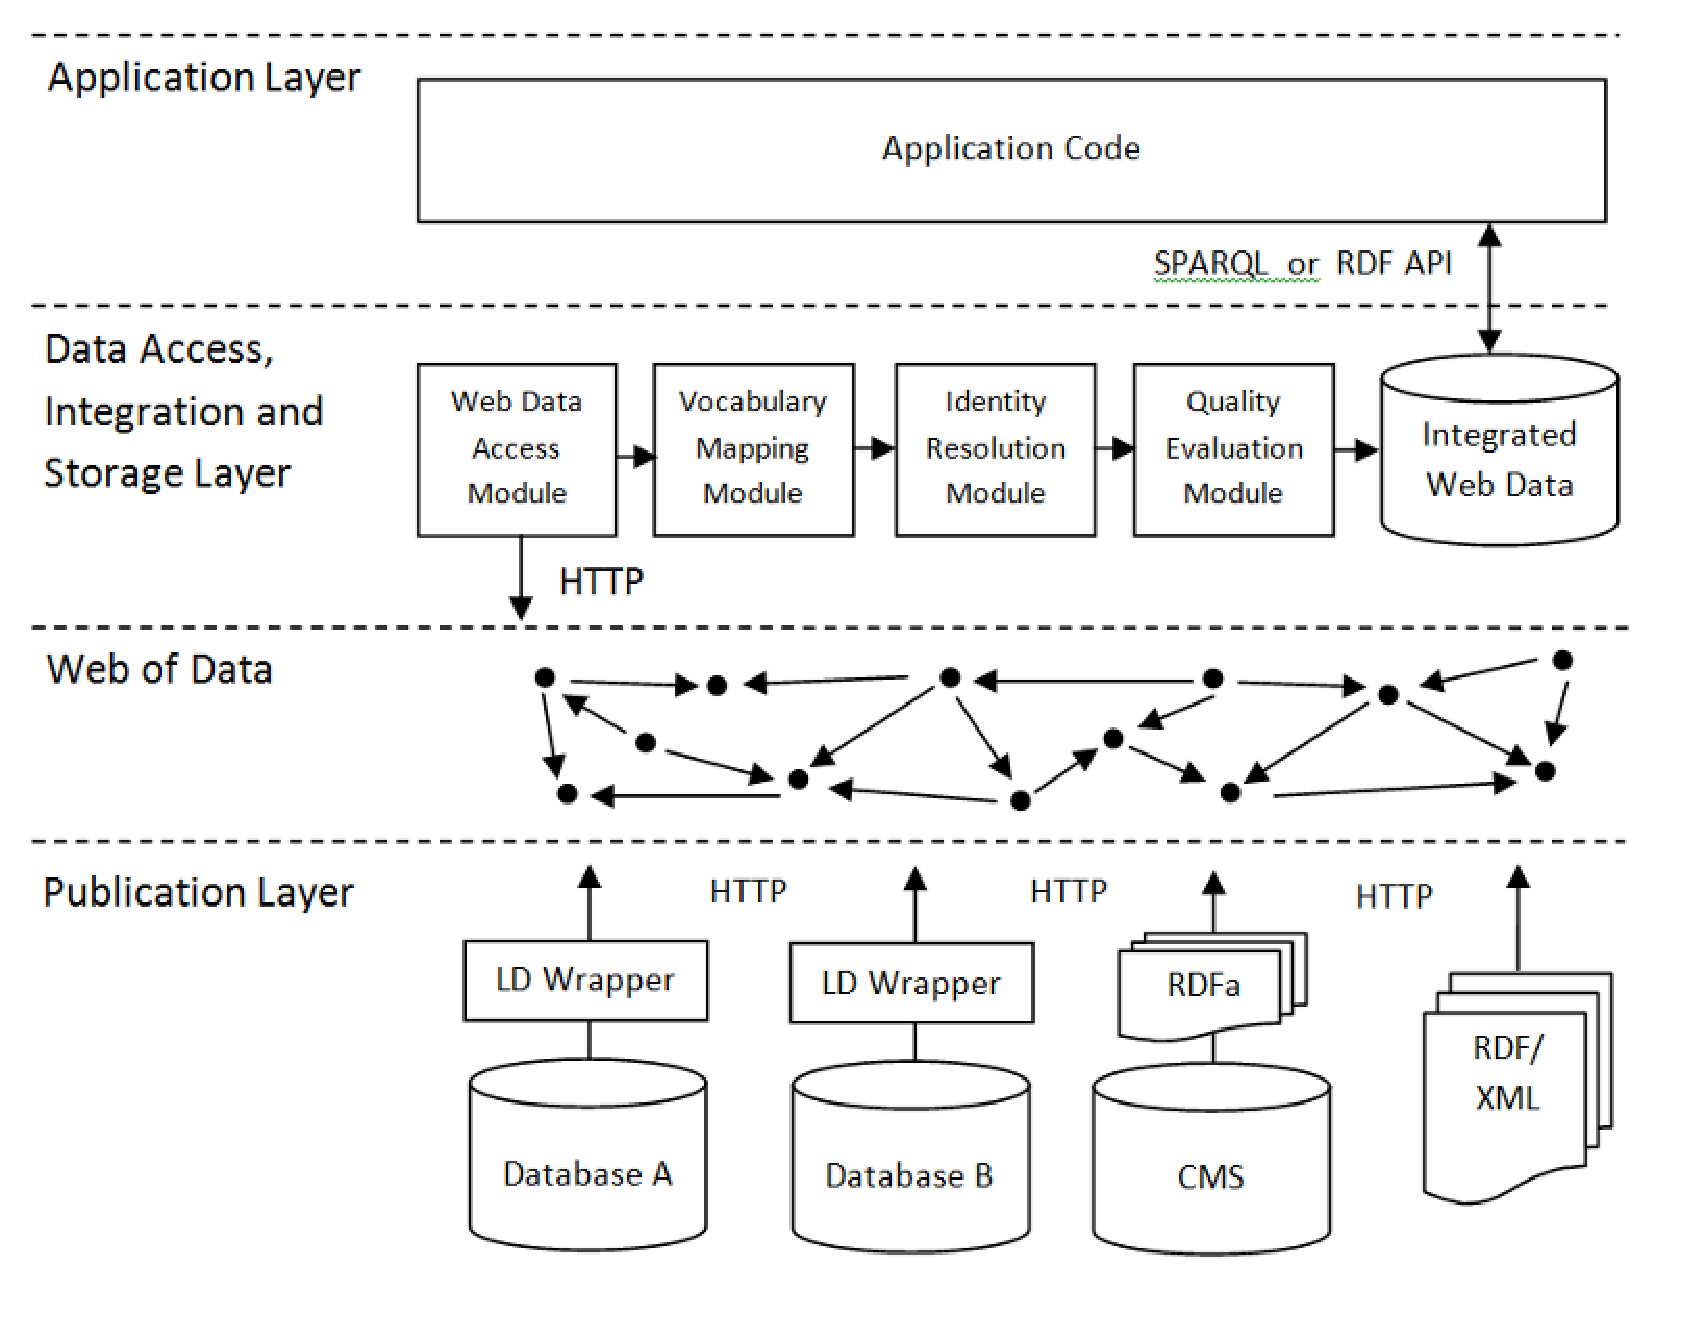
\includegraphics[width=10cm]{images/phd/Consumingarchitecture1_small}
\caption{\textit{Linked Data Publishing Options and Workflows} (extraída de \textit{Linked Data Design Considerations}).}
\label{fig:patterns-production}
\end{figure}

En conclusión, en este libro se ofrece una guía práctica y didáctica de los pasos a seguir para la aplicación
de la iniciativa de \linkeddata de forma correcta, asegurando las ventajas en los datos enlazados, minimizando las desventajas
y proveyendo un entorno para la generación de servicios de alto valor y calidad. 
Como podemos observar tanto las directrices de la Tabla~\ref{table:linkeddata-design-book}, como
los puntos a cumplir de la Tabla~\ref{table:linkeddata-check-list}, se pueden englobar en tres grandes procesos: producción,
publicación y consumo de \linkeddata. Especialmente hay que destacar los enfoques para la producción de \linkeddata desde
fuentes de datos ya existentes, ver Figura~\ref{fig:patterns-production} y Figura~\ref{fig:patterns-consum}.

\begin{figure}[!htb]
\centering
	\includegraphics[width=10cm]{images/phd/D2RServerArchitecture}
\caption{Architectura de D2R Server.}
\label{fig:patterns-consum}
\end{figure}


\subsubsection{\textit{Linked Data Patterns}}\label{linked-data-patterns}
Con el objetivo de proveer una forma estándar de transformar los datos
siguiendo la iniciativa de \linkeddata y disponer de unos criterios y soluciones estándar
para modelar, publicar y consumir datos, se han publicado una serie de patrones~\cite{linked-data-patterns} que resuelven
los problemas más comunes que se pueden encontrar. A continuación, ver Tabla~\ref{table:linkeddata-patterns}, se describen
algunos de los propuestos por los autores:


\begin{longtable}[c]{|l|p{7cm}|p{8cm}|} 

\hline

  \textbf{ID} & \textbf{Patrón} &  \textbf{Pregunta} \\\hline

\endhead
   1& \multicolumn{2}{|c|}{\textbf{\textit{Identifier Patterns}}}\\ \hline
  1.1 &  \textit{Hierarchical URIs} & \textit{How should URIs be assigned to a group of resources that form a natural hierarchy?}\\ \hline
  1.2 &  \textit{Literal Keys} & \textit{How do we publish non-global identifiers in \gls{RDF}?} \\ \hline
  1.3 &  \textit{Natural Keys} &  \textit{How can we create unique URIs from data that already has unique identifiers?} \\ \hline
  1.4 &  \textit{Patterned URIs} & \textit{How can we create more hackable, human-readable URIs?} \\ \hline
  1.5 &  \textit{Proxy URIs} & \textit{How do we deal with lack of standard identifiers for third-party resources?} \\ \hline
  1.6 &  \textit{Shared Keys} & \textit{How do we simplify the inter-linking of datasets?} \\ \hline
  1.7 &  \textit{URL Slug} &  \textit{How can we create \gls{URL}s from arbitrary text or keywords?} \\ \hline    
    2& \multicolumn{2}{|c|}{\textbf{\textit{Modelling Patterns}}}\\ \hline
  2.1 &  \textit{Custom Datatype} &  \textit{A data model contains structured values that don't correspond to one of the pre-existing \gls{XML Schema} datatypes.} \\ \hline    
  2.2 &  \textit{Index Resources} &  \textit{How can ordered collections or indexes be published as RDF?}  \\ \hline    
  2.3 &  \textit{Label Everything} & \textit{How can we ensure that every resource has a basic human-readable name?} \\ \hline     
  2.4 &  \textit{Link Not Label} &  \textit{How do we model a dataset to maximise benefits of a graph based model?} \\ \hline    
  2.5 &  \textit{Multi-Lingual Literal} & \textit{How can internationalized text be expressed in RDF? }\\ \hline    
  2.6 &  \textit{N-Ary Relation} & \textit{How can a complex relation, involving several resources, be modelled as RDF? }\\ \hline    
  2.7 &  \textit{Ordered List} &  \textit{How do we specify an ordering over a collection of resources?} \\ \hline     
  2.8 &  \textit{Ordering Relation} & \textit{How can we specify an ordering relationship between two or more resources?} \\ \hline     
  2.9 &  \textit{Preferred Label} &  \textit{How can a simple unambiguous label be provided for a resource? }\\ \hline    
  2.10 &  \textit{Qualified Relation} &  \textit{How can we describe or qualify a relationship between two resources?} \\ \hline   
  2.11 &  \textit{Reified Statement} &  \textit{How can we make statements about statements?} \\ \hline    
  2.12 &  \textit{Topic Relation} &  \textit{How can a web page or document be associated with a resource?} \\ \hline      
  2.13 &  \textit{Typed Literal} &  \textit{How can a datatype be associated with an RDF literal?} \\ \hline        
    3& \multicolumn{2}{|c|}{\textbf{\textit{Publishing Patterns}}}\\ \hline
  3.1 &  \textit{Annotation} &  \textit{How can data about third-party resources be published as part of a dataset?}  \\ \hline    
  3.2 &  \textit{Autodiscovery} &   \textit{How can people find the underlying linked data for a given web page?}  \\ \hline    
  3.3 &  \textit{Document Type} & \textit{How can some context be provided about a set of RDF triples published to the web?} \\ \hline     
  3.4 &  \textit{Edit Trail} &  \textit{How can people be encouraged to improve or fix up open data?} \\ \hline    
  3.5 &  \textit{Embedded Metadata} &  \textit{How do we add structured data to an existing document or file?} \\ \hline    
  3.6 &  \textit{Equivalence Links} &  \textit{How do we indicate that different \gls{URI}s refer to the same resource or concept?} \\ \hline    
  3.7 &  \textit{Link Base} &  \textit{How can outbound links from a dataset be managed separately from the core data?} \\ \hline     
  3.8 &  \textit{Materialize Inferences} &  \textit{How can data be published for use by clients with limited reasoning capabilities?} \\ \hline     
  3.9 &  \textit{Named Graphs} & \textit{How do we organize and annotate a set of RDF statements?} \\ \hline    
  3.10 &  \textit{Primary Topic Autodiscovery} & \textit{How can people identify the principal subject of a given web page?}  \\ \hline    
  3.11 &  \textit{Progressive Enrichment} &  How can the quality of data or a data model be improved over time? \\ \hline      
  3.12 &  \textit{See Also} & \textit{How can RDF documents be linked together to allow crawlers and user agents to navigate between them?} \\ \hline    
        4& \multicolumn{2}{|c|}{\textbf{\textit{Application Patterns}}}\\ \hline
  4.1 &  \textit{Assertion Query} & \textit{How can a dataset be tested for known patterns?} \\ \hline    
  4.2 &  \textit{Blackboard} &  \textit{How can the task of compiling or constructing a dataset be divided up into smaller tasks?}\\ \hline    
  4.3 &  \textit{Bounded Description} & \textit{How can we generate a useful default description of a resource without having to enumerate all the properties or relations that are of interest?} \\ \hline     
  4.4 &  \textit{Composite Descriptions} &  \textit{How do we declare the underlying dataset for a page involving custom subsets or views of the data?}\\ \hline    
  4.5 &  \textit{Follow Your Nose} &  \textit{How do we find additional relevant data from the web?} \\ \hline    
  4.6 &  \textit{Missing Isn't Broken} &  \textit{How do we handle the potentially messy or incomplete data we use from the web?} \\ \hline    
  4.7 &  \textit{Parallel Loading} &  \textit{How can we reduce loading times for a web-accessible triple store?} \\ \hline     
  4.8 &  \textit{Parallel Retrieval} & \textit{ How can we improve performance of an application dynamically retrieving Linked Data?} \\ \hline     
  4.9 &  \textit{Resource Caching} &  \textit{How can an application that relies on loading data be more tolerant of network failures and/or reduce use of bandwidth} \\ \hline    
  4.10 &  \textit{Schema Annotation} & \textit{How can application-specific processing rules be externalized?} \\ \hline    
  4.11 &  \textit{Smushing} &  \textit{How do we merge data about resources that may not be consistently identified?} \\ \hline
  4.12 &  \textit{Transformation Query} & \textit{How can we normalize or transform some RDF data so that it conforms to a preferred model?} \\ \hline        
 
\hline
\caption{\textit{Linked Data Patterns}}\label{table:linkeddata-patterns}\\    
\end{longtable}

Al igual que en el caso anterior, en estos patrones se ofrecen una serie de guías para resolver problemas comunes
que surgen en el momento de producir, publicar y consumir datos enlazados. Suponen una información muy valiosa, ya que
permiten homogeneizar la creación de datos enlazados de tal forma que si una persona u organización asegura que ha 
seguido estos principios, se pueden construir aplicaciones que sepan qué tipo de datos se van encontrar y cómo, disminuyendo
así el coste de reutilización de datos provenientes de terceros y asegurar la calidad de los mismos.

\subsubsection{\textit{Best Practices} del W3C}
Se trata de una serie de documentos y buenas prácticas~\cite{best-gld} dentro del 
grupo de trabajo del \gls{W3C} \textit{Government Linked Data Working Group}~\cite{gld-group} cuya actividad se lanzó
 en el \textit{Face 2 Face} de junio de 2011 y que consta de los siguientes objetivos:

\begin{itemize}
 \item \textit{The overarching objective is to provide best practices and guidance to create of high quality, re-usable Linked Open Data (LOD)}.
 \item \textit{Description of the full life cycle of a Government Linked Data project, starting with identification of suitable data sets, procurement, modeling, vocabulary selection, through publication and ongoing maintenance.}
 \item \textit{Definition of known, proven steps to create and maintain government data sets using Linked Data principles.}
  \item \textit{Guidance in explaining the value proposition for LOD to stakeholders, managers and executives.}
  \item \textit{Assist the Working Group in later stages of the Standards Process, in order to solicit feedback, use cases, etc.}
\end{itemize}

Como grupo de trabajo su esfuerzo se centrará en cumplir los objetivos establecidos a través de la consecución de materiales como 
recomendaciones, notas, etc., en los siguientes ámbitos:
\begin{enumerate}
 \item  \textit{Procurement.}
 \item  \textit{Vocabulary Selection.}
 \item \textit{URI Construction.}
   \item \textit{Versioning.}
   \item \textit{Stability.}
   \item \textit{Legacy Data.}
   \item \textit{Cookbook.} 
\end{enumerate}

Evidentemente y teniendo en cuenta los participantes en esta actividad, está claro que los puntos de actuación
seleccionados son claramente estratégicos para la iniciativa de \linkeddata y es por ello que aunque
los resultados están en una etapa previa, es conveniente sumamente atento a sus resultados con el doble objetivo
de por una parte aplicarlos a futuros proyectos y por otra parte realimentar el esfuerzo realizado por sus participantes.

\subsubsection{\textit{Linked Data Cookbook} del W3C}\label{linked-data-cookbook}
Uno de los esfuerzos de la actividad comentada en la sección anterior, consiste
en la elaboración de un libro de buenas prácticas~\cite{linked-data-cookbook} en cuanto a la producción, publicación y consumo de 
datos enlazados. Para ello se recopilarán las prácticas más comunes
desde el punto de vista de la ingeniería que faciliten la adopción de \linkeddata en 
diferentes entornos, asegurando una calidad y previniendo que el uso de datos enlazados
no sea sinónimo de depuración.

Con carácter previo se han fijado una serie de pasos que se han de seguir para desplegar
una infraestructura de datos enlazados acompañada de una serie de prácticas que aseguren
la calidad y el proceso de adopción. Esta iniciativa es compatible con las buenas prácticas
vista en las Secciones~\ref{linked-data-design-issues} y~\ref{linked-data-patterns} y además
ofrece una buena guía de todos los puntos que hay que tener en cuenta: diseño de URIs, vocabularios
a reutilizar, herramientas, etc. Actualmente estas prácticas se están desarrollando y 
se dividen en $7$ pasos que se presentan en la Tabla~\ref{table:linkeddata-practices}.


\begin{longtable}[c]{|l|p{7cm}|p{8cm}|} 

\hline

  \textbf{ID} & \textbf{Práctica} & \textbf{Descripción} \\\hline

\endhead
  1 &  \textit{Model the Data} & \textit{Identify, Model, Name and Test.}\\ \hline
  2 &  \textit{Name things with \gls{URI}s} & \textit{Following a name convention of current guides.} \\ \hline
  3 &  \textit{Re-use vocabularies whenever possible} &   \textit{Any given Linked Data set may include terms from an existing and widely used vocabulary.} \\ \hline
  4 &  \textit{Publish human and machine readable descriptions} & \textit{Self-describing data suggests that ''information about the encodings used for each representation is provided explicitly within the representation``}.  \\ \hline
  5 &  \textit{Convert data to \gls{RDF}} & N/A \\ \hline
  6 &  \textit{Specify an appropriate license} & N/A \\ \hline
  7 &  \textit{Announce the new Linked Data Set(s) } &  N/A  \\ \hline    
 
\hline
\caption{\textit{The 7 Best Practices for Producing Linked Data.}}\label{table:linkeddata-practices}\\    
\end{longtable}


\subsubsection{\textit{Government Linked Data-Life Cycle}}\label{gld}
Siguiendo con las actividades que se desarrollan en este grupo de trabajo del W3C sobre datos enlazados
en el entorno de la administración pública electrónica, se han identificado los siguientes ciclos de vida~\cite{gld-lifecycle} propuestos
por diversos autores:

\begin{itemize}
 \item Bernadette Hyland, ver Figura~\ref{fig:hyland}. 

\begin{figure}[!htb]
\centering
	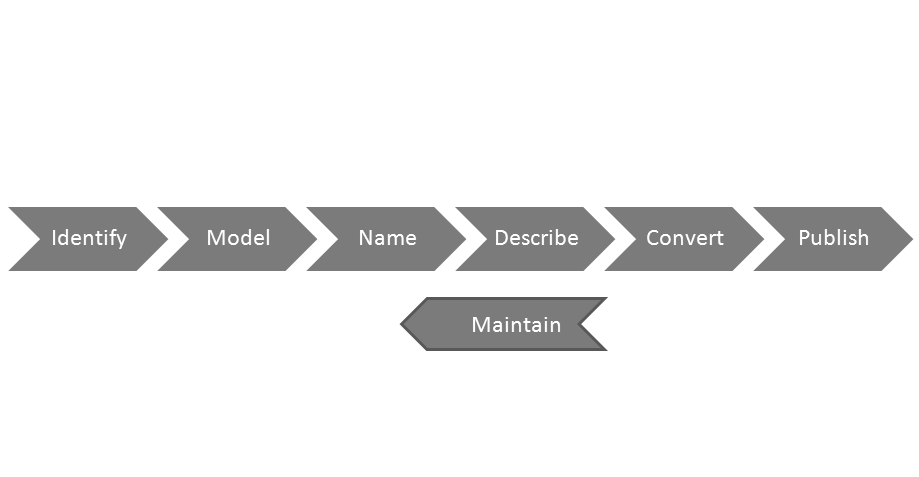
\includegraphics[width=14cm]{images/phd/Hyland}
\caption{\textit{Linked Data Lifecycle by B. Hyland}.}
\label{fig:hyland}
\end{figure}


 \item Michael Hausenblas, ver Figura~\ref{fig:hausenblas}.

\begin{figure}[!htb]
\centering
	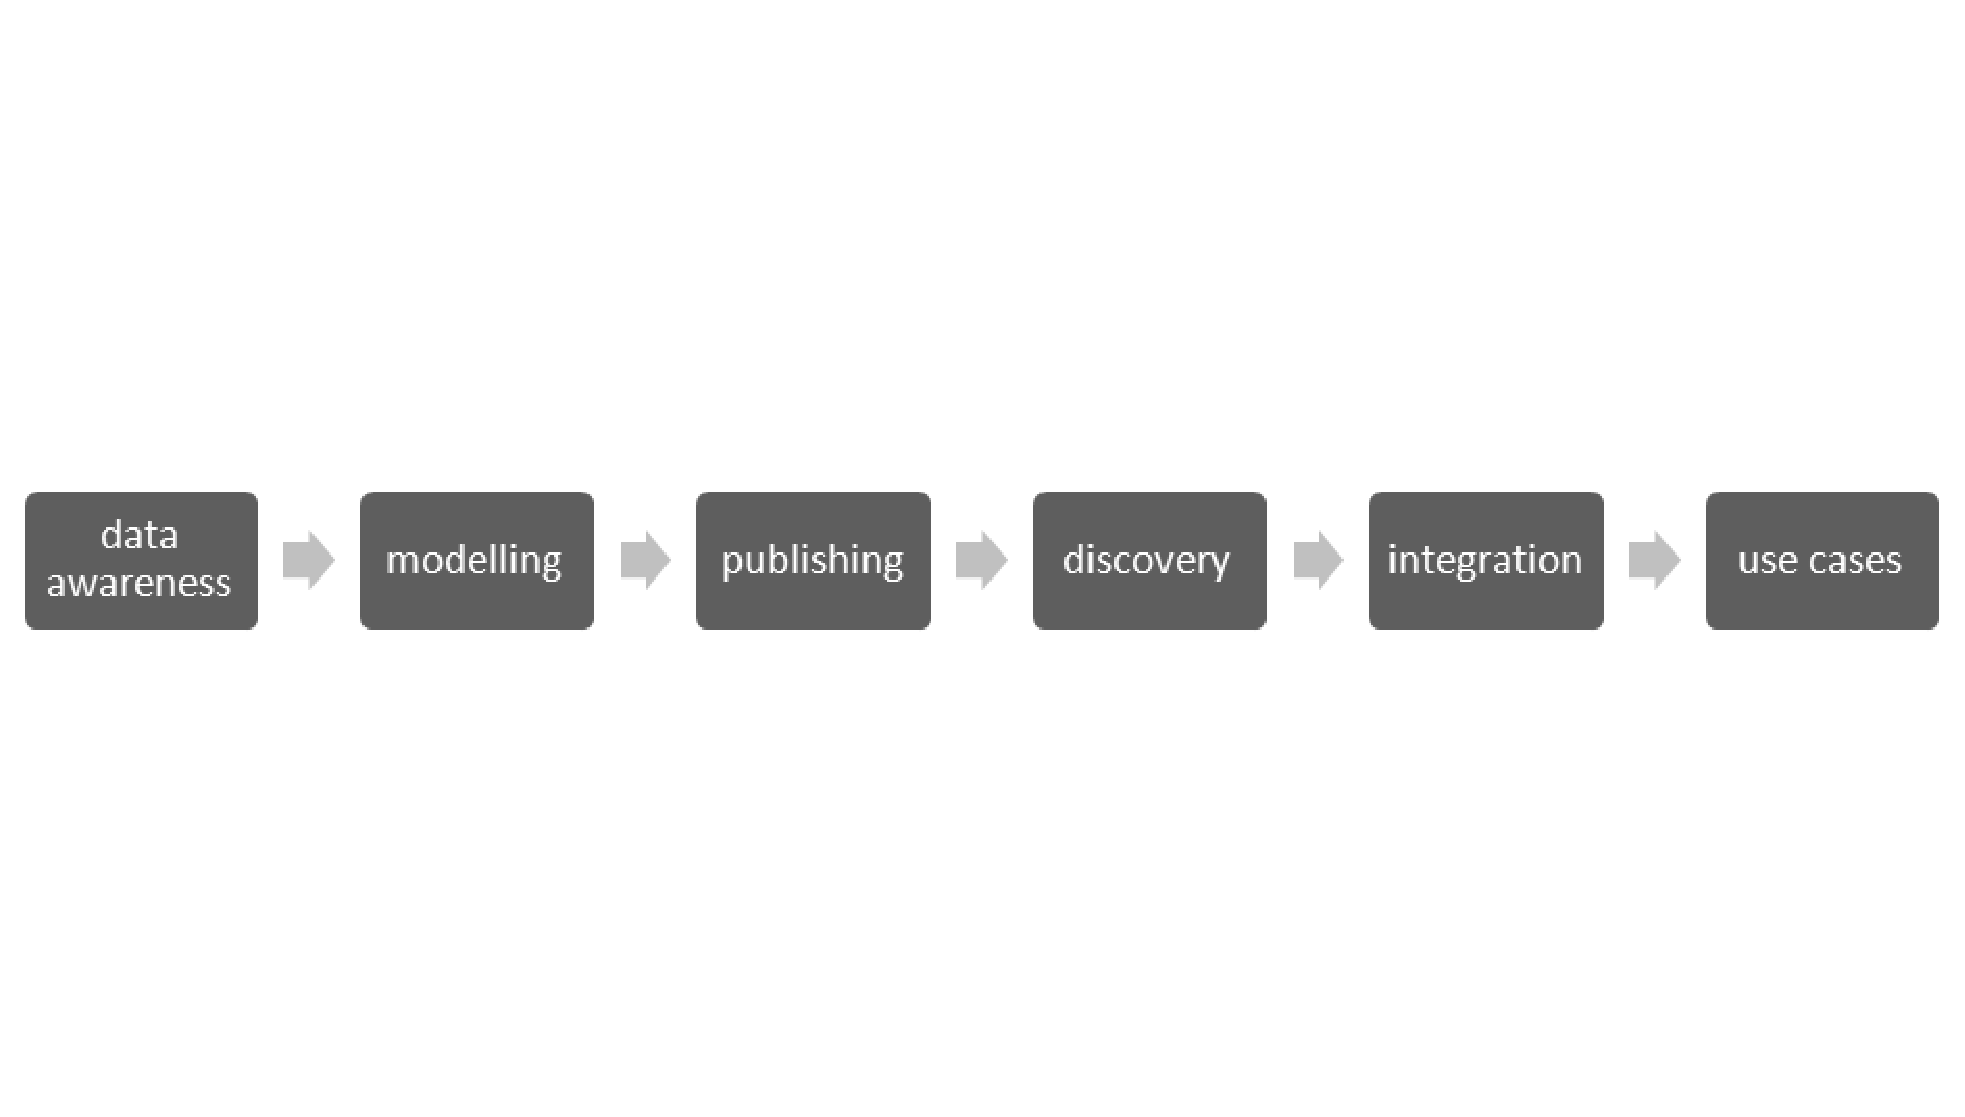
\includegraphics[width=14cm]{images/phd/Hausenblas}
\caption{\textit{Linked Data Lifecycle by M. Hausenblas}.}
\label{fig:hausenblas}
\end{figure}


 \item Boris Villazón-Terrazas, ver Figura~\ref{fig:boris}

\begin{figure}[!htb]
\centering
	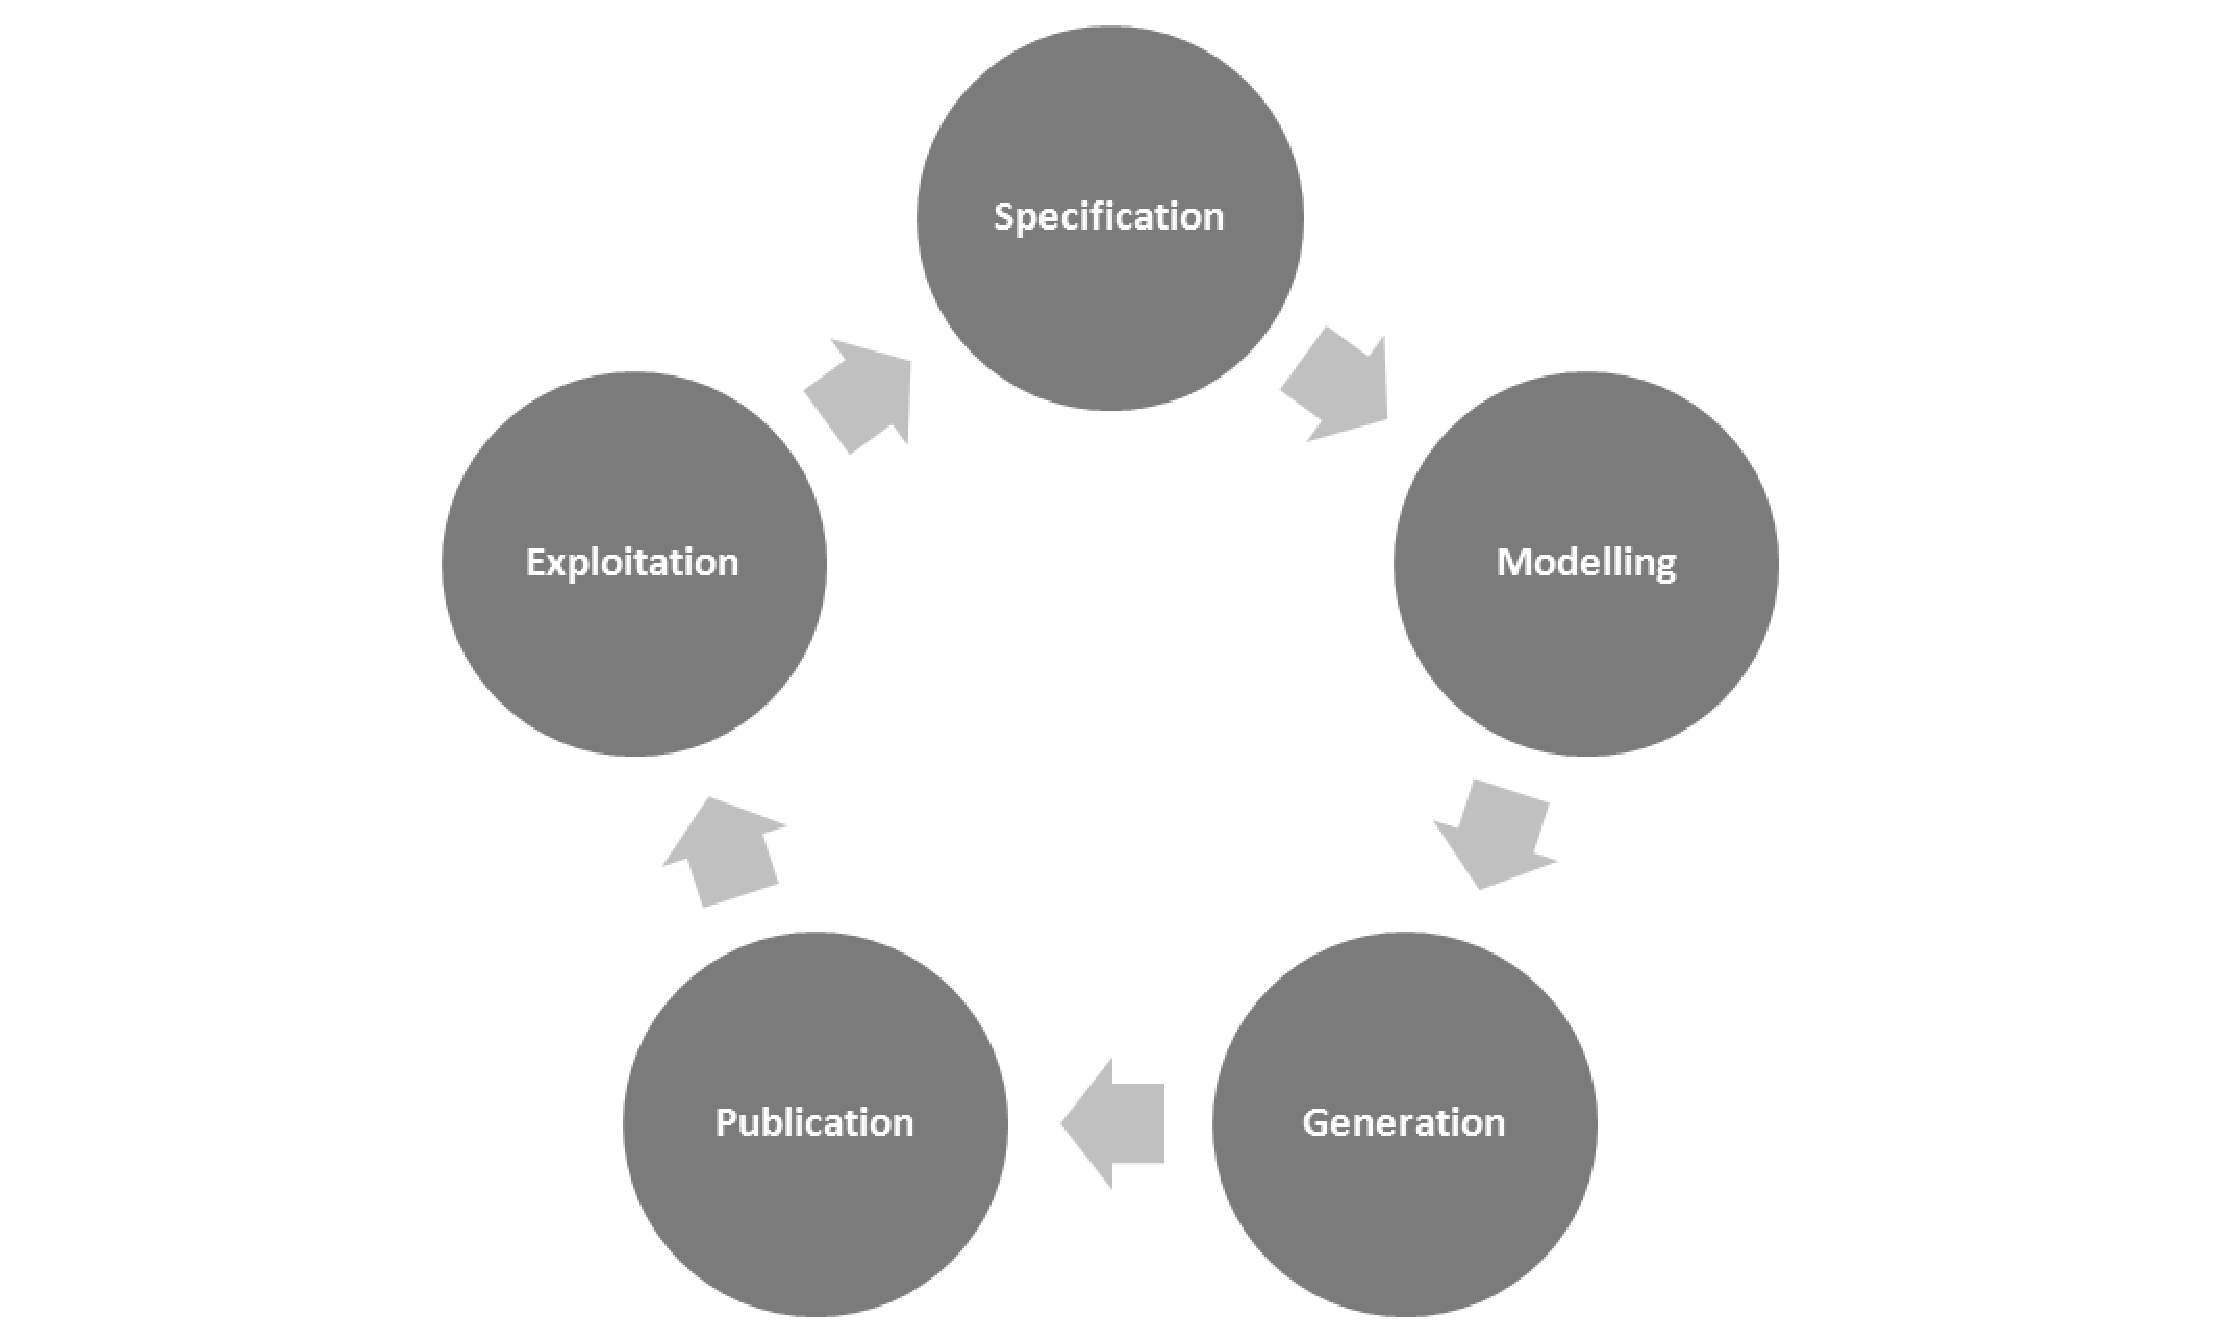
\includegraphics[width=14cm]{images/phd/Villazon-terrazas}
\caption{\textit{Linked Data Lifecycle by B. Villazón-Terrazas}.}
\label{fig:boris}
\end{figure}


 \item \textit{The DataLift Vision}, ver Figura~\ref{fig:datalift} 

\begin{figure}[!htb]
\centering
	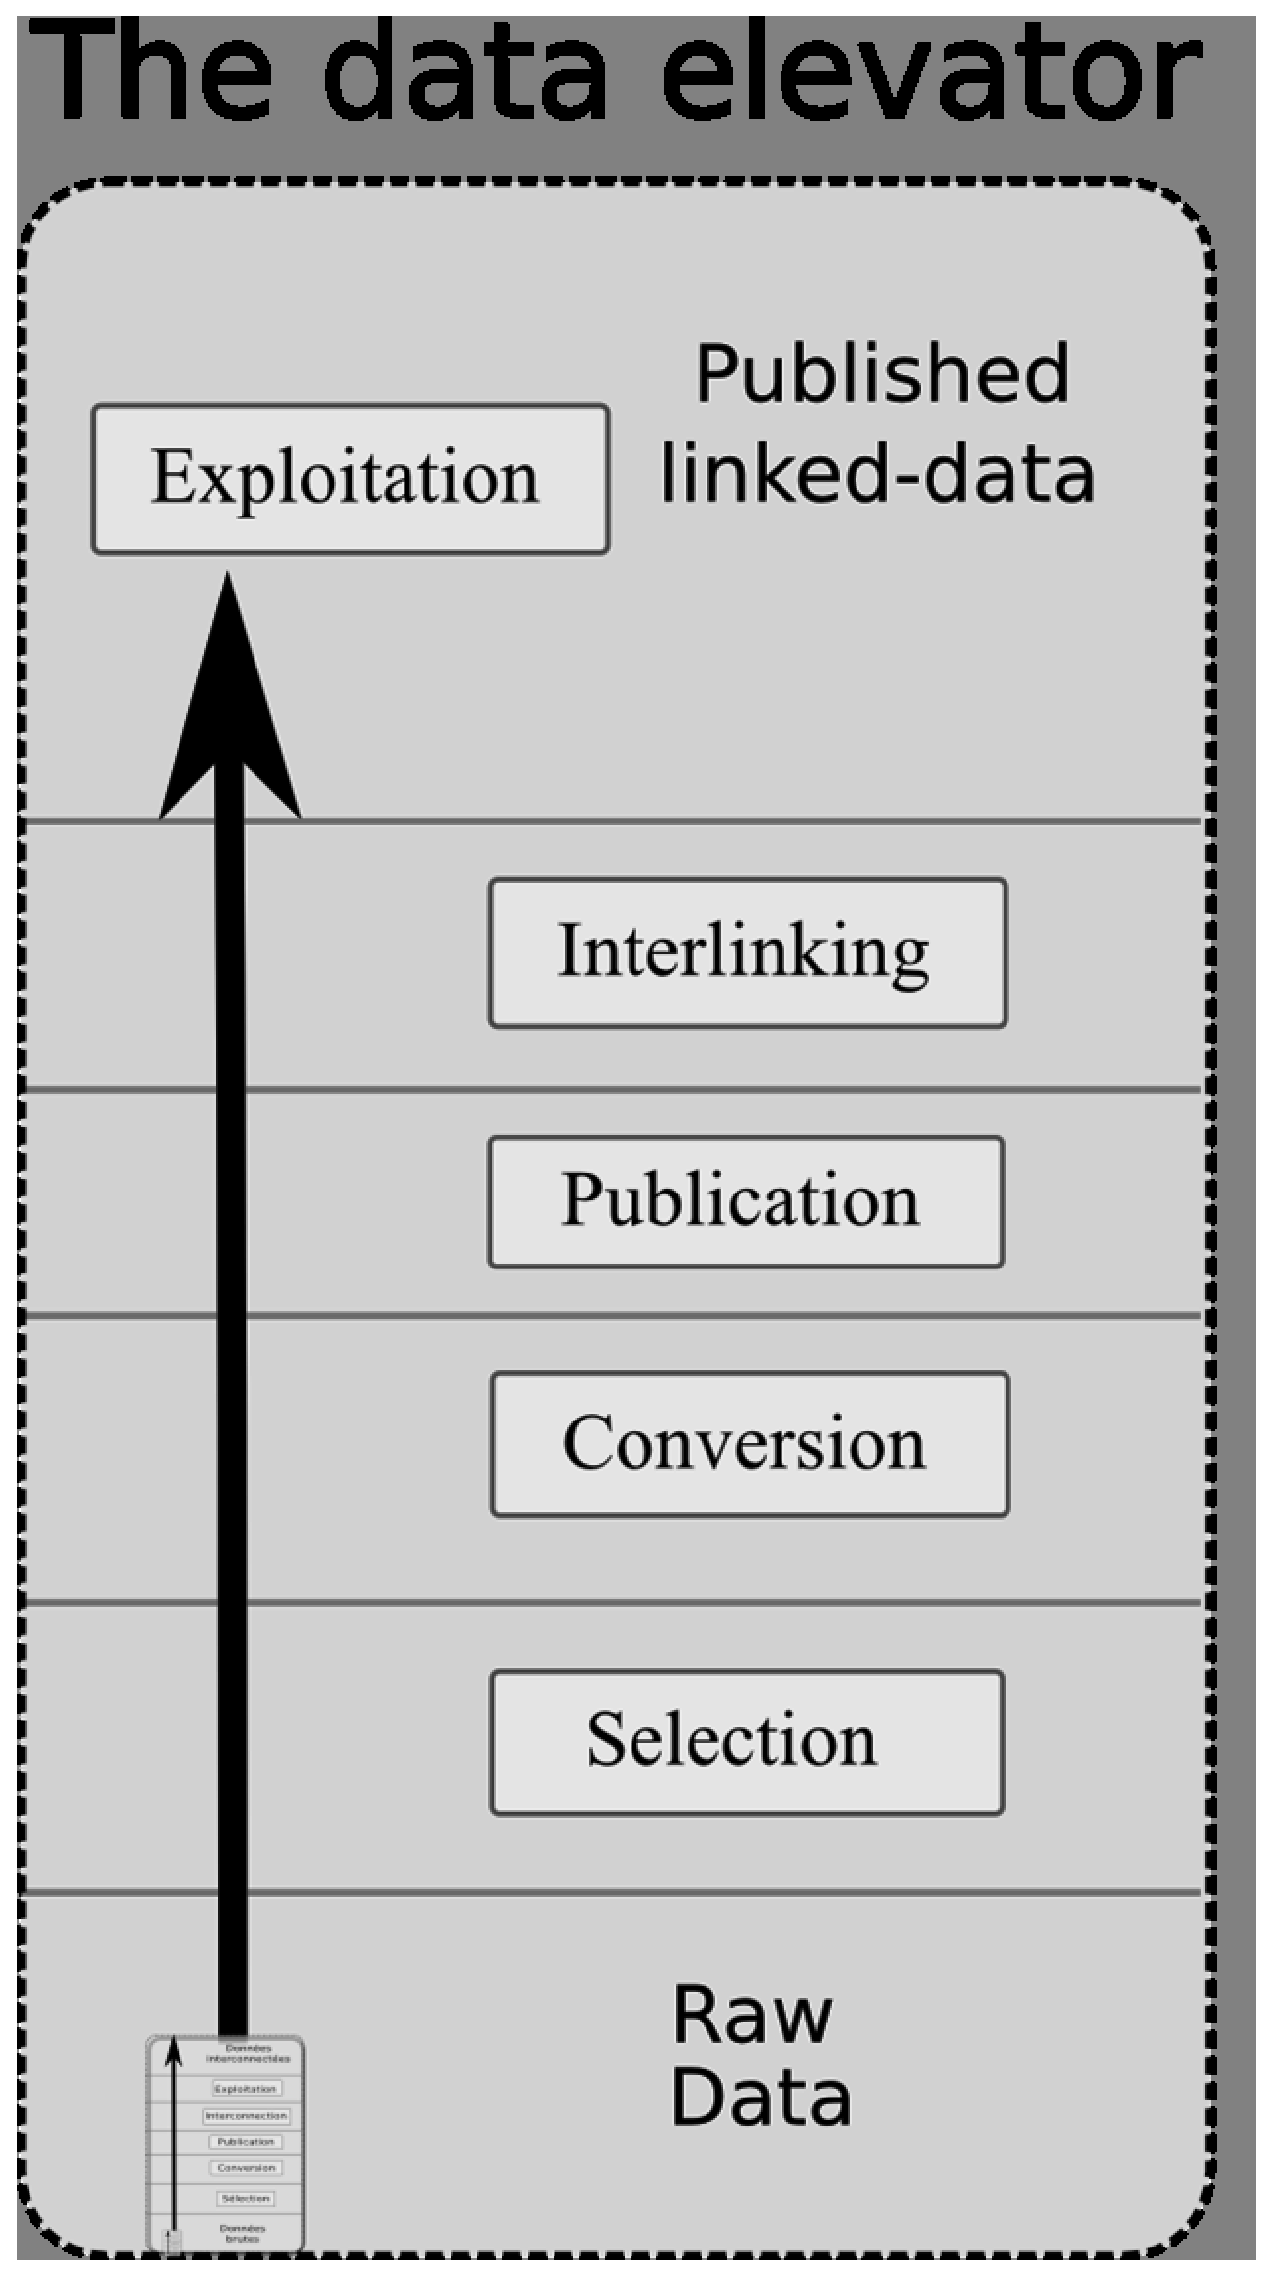
\includegraphics[width=6cm]{images/phd/Data_elevator}
\caption{\textit{DataLift Vision}.}
\label{fig:datalift}
\end{figure}
 \end{itemize}


En todos ellos se recogen en grandes procesos los pasos a seguir para desplegar el modelo de \linkeddata en una organización. Aunque
existan cambios en la denominación, en el nivel de abstracción o en el orden de algunos procesos, el objetivo coincide en todos ellos. No obstante, estos modelos han surgido, probablemente,
de la experiencia propia de los autores y aún estando en su etapa de desarrollo suponen un avance para afrontar la implantación
de \linkeddata como un proceso de ingeniería cuantificable.

\subsubsection{\textit{Publishing Open Government Data} del W3C}
Se trata de un borrador de trabajo~\cite{publishing-ogd} (\textit{W3C Working Draft 8 September 2009}) del grupo del \gls{W3C} \textit{\gls{eGovernment} Interest Group} en el cual
se hace una descripción somera sobre cómo publicar datos gubernamentales en la web. Reseñan fundamentalmente una serie de pasos 
para publicar datos sin grandes restricciones y de forma ágil, basándose en 3 pasos,
 ver Tabla~\ref{table:publish-ogd}, de carácter general pero que pueden servir especialmente a perfiles
no técnicos presentes en las instituciones públicas.

\begin{longtable}[c]{|l|p{7cm}|p{8cm}|} 
\hline
  \textbf{ID} & \textbf{Paso} & \textbf{Descripción} \\\hline
\endhead
  1 &  \textit{Step 1} & \textit{The quickest and easiest way to make data available on the Internet is to publish the data in its raw form.}\\ \hline
  2 &  \textit{Step 2} & \textit{Create an online catalog of the raw data (complete with documentation) so people can discover what has been posted.} \\ \hline
  3 &  \textit{Step 3} &   \textit{Make the data both human- and machine-readable.} \\ \hline
\hline
\caption{\textit{Straightforward Steps to Publish Government Data.}}\label{table:publish-ogd}\\    
\end{longtable}

De la misma forma, en el propio documento se exponen otros factores a tener en el momento
de publicación de los de datos y que van en la línea de la iniciativa de \linkeddata. Simplemente se trata
de una guía básica prácticamente de carácter divulgativo.

\subsubsection{\textit{LOD2 Stack}}\label{lod2-project}
Dentro del proyecto europeo LOD2~\cite{lod2-project} con nº de contrato: 257943, una duración desde septiembre de 2010
hasta agosto de 2014 y una financiación de más de $7$ millones euros se está desarrollando
una serie de documentos y tecnología asociada a la iniciativa de \lod con el objetivo de proveer
buenas prácticas y herramientas que den soporte a toda la cadena de producción, publicación y consumo
de datos enlazados en distintos dominios. Uno de los últimos resultados que han conseguido y que
se encuentra en continua evolución es la denominada \textit{LOD2 Stack}~\cite{lod2-stack} que contiene una
serie de herramientas para cada una de las etapas necesarias en la apertura de datos como \linkeddata.
Según la arquitectura de alto nivel, ver Figura~\ref{fig:lod-arch}, se identifican los siguientes componentes.

\begin{description}
 \item [\textit{OntoWiki}~\cite{tramp-s-2010-ekaw-demo}.] \textit{OntoWiki is a tool providing support for agile, distributed knowledge engineering scenarios}. 
 \item [\textit{PoolParty}~\cite{poolparty}.] \textit{PoolParty is a thesaurus management system and a SKOS editor for the Semantic Web including text mining and linked data capabilities.}
 \item [\textit{Sig.ma}~\cite{citeulike:8529753}.] \textit{Sig.ma is a tool to explore and leverage the Web of Data.}
 \item [\textit{Comprehensive Knowledge Archive Network (CKAN)~\cite{ckan}}.] \textit{CKAN is a registry or catalogue system for datasets or other ''knowledge'' resources.}
 \item [\textit{D2R Server}~\cite{Bizer_Cyganiak_2006}.] \textit{D2R Server is a tool for publishing relational databases on the Semantic Web. }
 \item [\textit{DBpedia Extraction}~\cite{Bizer:2009:D-C:1640541.1640848}.] \textit{DBpedia is a community effort to extract structured information from Wikipedia and to make this information available on the Web.}
 \item [\textit{DL-Learner}~\cite{lehmann2009}.] \textit{DL-Learner is a tool for supervised Machine Learning in OWL and Description Logics.}
 \item [\textit{MonetDB}~\cite{Boncz06monetdb/xquery:a}.] \textit{MonetDB is an open-source high-performance database system that allows to store relational, XML and RDF data}.
 \item [\textit{SemMF}.] \textit{SemMF is a flexible framework for calculating semantic similarity between objects that are represented as arbitrary RDF graphs.}
 \item [\textit{Silk Framework}~\cite{www2009227}.] \textit{The Silk Linking Framework supports data publishers in setting explicit RDF links between data items within different data sources.}
 \item [\textit{Sindice}~\cite{TummarelloDO07}.] \textit{Sindice is a state of the art infrastructure to process, consolidate and query the Web of Data. }
 \item [\textit{Sparallax}~\cite{Sparallax}.] \textit{Sparallax is a faceted browsing interface for SPARQL endpoints, based on Freebase Parallax.}
 \item [\textit{Triplify}~\cite{Triplify}.] \textit{Triplify provides a building block for the ``semantification'' of Web applications.}
 \item [\textit{OpenLink Virtuoso}~\cite{Virtuoso}.] \textit{Virtuoso is a knowledge store and virtualization platform that transparently integrates Data, Services, and Business Processes across the enterprise.}
 \item [\textit{WIQA}~\cite{wiqa}.] \textit{The Web Information Quality Assessment Framework is a set of software components that empowers information consumers to employ a wide range of different information quality assessment policies to filter information from the Web.} 
\end{description}

\begin{figure}[!htb]
\centering
	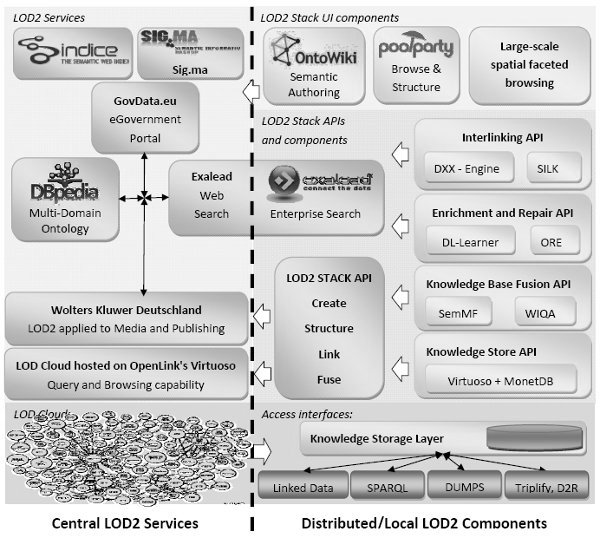
\includegraphics[width=10cm]{images/phd/lod2-high-level-architecture}
\caption{\textit{LOD2 high-level Architecturel} (extraída del portal del proyecto LOD2).}
\label{fig:lod-arch}
\end{figure}


Como se puede observar este grupo de herramientas dan soporte a todo el ciclo de vida de los datos enlazados y proveen
una plataforma genérica en la cual cualquier persona o entidad pueda integrar un nuevo conjunto de datos, desde
recursos ya disponibles en \gls{RDF} hasta documentos de texto. La realización de este proyecto es de una suma transcendencia
para la comunidad, ya que en el despliegue de una infraestructura basada en datos enlazados se suele incurrir en las mismas
dudas y problemas, por lo que el disponer de una guía que parta desde un punto de vista teórico hasta su realización práctica, 
supone una gran avance respecto a las especificaciones teóricas, recetas y buenas prácticas que se han mencionado en las
secciones anteriores. 

Por otra parte, las herramientas desarrolladas se encuentran enclavadas dentro de un proceso o ciclo de vida de datos enlazados,
ver Figura~\ref{fig:lod-lifecycle}. Se trata de un modelo iterativo y realimentado, en el cual se van pasando por distintas fases
para cumplir con la producción, publicación y consumo de datos, utilizando las herramientas previamente comentadas y atacando
las principales barreras que se suelen encontrar, así como aplicando los principios de diseño de \linkeddata.

\begin{figure}[!htb]
\centering
	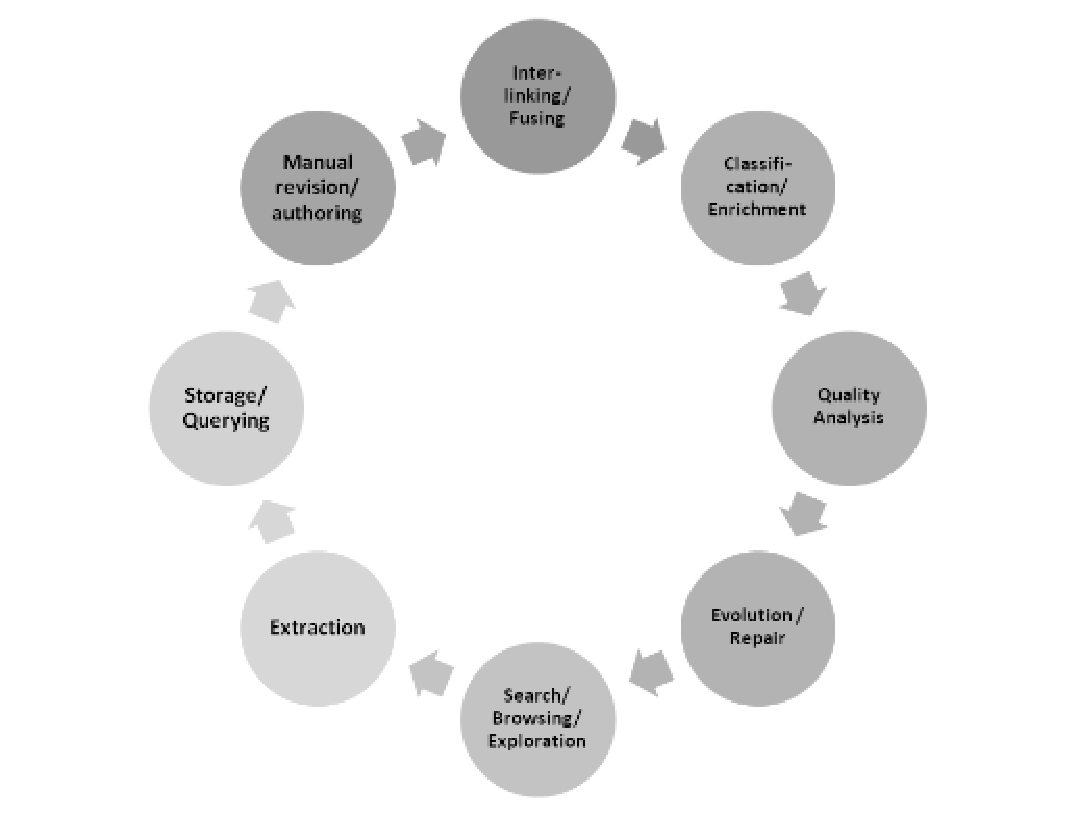
\includegraphics[width=12cm]{images/phd/lod-lifecycle-small}
\caption{\textit{Linked Data LifeCycle} (extraída de LOD2 Demo).}
\label{fig:lod-lifecycle}
\end{figure}

Para la aplicación de los principios de \linkeddata es realmente conveniente prestar atención al trabajo
desarrollado en este proyecto, no obstante, teniendo en cuenta que tan sólo se cuenta con un año de desarrollo
es complicado aplicar su enfoque de forma integral.

\subsubsection{\textit{Toward a Basic Profile for Linked Data} de IBM}
Dentro de la actividad de IBM en el campo de \linkeddata, se ha identificado
la necesidad de fijar una serie de reglas para aplicar esta iniciativa de forma
cuantificable. El objetivo de esta guía es llegar a introducir dentro de una herramienta
como \textit{Rationale} (también perteneciente a IBM) el modelo arquitectónico propuesto por los datos
enlazados, cumpliendo las directrices de la misma con la meta de obtener
la tecnología necesaria que sirva para integrar datos de forma ágil en las aplicaciones.

El término utilizado por IBM es ``Basic Profile Resources''~\cite{basic-profile-ibm} que se define como recursos \linkeddata accesibles mediante HTTP que siguen una serie de patrones
y convenciones comunes. En general, estos recursos dependen del dominio en el cual
estén definidos y tan sólo se delimitan como comunes unos pocos que se consideran
transversales a cualquier dominio. Estos recursos siguen una serie de reglas, ver Tabla~\ref{table:basic-ibm}, y reutilizan
vocabularios existentes con el objetivo de cumplir con la iniciativa de \linkeddata. 

\begin{longtable}[c]{|l|p{7cm}|p{8cm}|} 
\hline
  \textbf{ID} & \textbf{Rule} & \textbf{Descripción} \\\hline
\endhead
  1 &  \textit{Basic Profile Resources are \gls{HTTP} resources} & \textit{They can be created, modified, deleted and read using standard HTTP methods.}\\ \hline
  2 &  \textit{Basic Profile Resources use \gls{RDF} to define their states} & \textit{The state of a Basic Profile Resource (in the sense of state used in the REST architecture) is defined by a set of RDF triples.} \\ \hline
  3 &  \textit{You can request an RDF/XML representation of any Basic Profile Resource} &   \textit{The resource might have other representations.} \\ \hline
  4 &  \textit{Basic Profile clients use Optimistic Collision Detection during update} &   \textit{Because the update process involves getting a resource first, and then modifying it and later putting it back on the server, there is the possibility of a conflict (for example, another client might have updated the resource since the GET action). To mitigate this problem, Basic Profile implementations should use the HTTP If-Match header and HTTP ETags to detect collisions.} \\ \hline
  5 &  \textit{Basic Profile Resources use standard media types} &   \textit{ Basic Profile does not require and does not encourage the definition of any new media types.} \\ \hline
  6 &  \textit{Basic Profile Resources use standard vocabularies} &   \textit{Basic Profile Resources use common vocabularies (classes, properties, and so forth) for common concepts.} \\ \hline
  7 &  \textit{Basic Profile Resources set \texttt{rdf:type} explicitly.} &   \textit{A resource's membership in a class extent can be derived implicitly or indicated explicitly by a triple in the resource representation.} \\ \hline
  8 &  \textit{Basic Profile Resources use a restricted number of standard data types} &   \textit{RDF does not define data types to be used for property values, so Basic Profile lists a set of standard datatypes to be used in Basic Profile.} \\ \hline
  9 &  \textit{Basic Profile clients expect to encounter unknown properties and content} &   \textit{Basic Profile provides mechanisms for clients to discover lists of expected properties for resources for particular purposes.} \\ \hline
  10 &  \textit{Basic Profile clients do not assume the type of a resource at the end of a link} &   \textit{Many specifications and most traditional applications have a "closed model," by which we mean that any reference from a resource in the specification or application necessarily identifies a resource in the same specification.} \\ \hline
  11 &  \textit{Basic Profile servers implement simple validations for Create and Update} &   \textit{Basic Profile servers should try to make it easy for programmatic clients to create and update resources.} \\ \hline
  12 &  \textit{Basic Profile Resources always use simple RDF predicates to represent links} &   \textit{Basic Profile makes it very simple to know how links will appear in representations and also makes it very simple to query them.} \\ \hline
\hline
\caption{\textit{Basic Profile Resources.}}\label{table:basic-ibm}\\    
\end{longtable}

Repasando esta lista de reglas se puede observar como algunas afectan a los principios $2º$ y $3º$ de \linkeddata sin
modificar su significado pero especificando de forma más concreta el funcionamiento esperado. La importancia
de este reciente artículo reside en varios puntos: es realizado por IBM, es coherente con las reglas de \linkeddata y
ofrece un carácter práctico desde el punto de vista de la ingeniería para implementar, o en este caso, incluir
la arquitectura y modelo de trabajo de datos enlazados en una plataforma existente como es \textit{Rationale}.


\subsubsection{Metodología y Proceso de Adopción de \linkeddata en la Biblioteca del Congreso de Chile}
En este trabajo se propone una metodología~\cite{DBLP:conf/i-semantics/Cifuentes-SilvaSG11,methodologyCaepia2011} y proceso de adopción de la iniciativa de \linkeddata en el contexto
de las Administraciones Públicas y concretamente en la Biblioteca del Congreso de Chile para la publicación
de la legislación actual e histórica. En general, se trata en realidad de la especificación de una infraestructura
para dar soporte a los datos enlazados y un proceso de generación con diferentes etapas, que parten de un
caso particular motivador pero que se podrían aplicar a un contexto genérico. En la Figura~\ref{fig:bcn-infraestructura} se
pueden observar los distintos componentes que se proponen y que encajan con la infraestructura propuesta en 
el proyecto LOD2, ver Sección~\ref{lod2-project}. Una de las diferencias reside en las herramientas seleccionadas
para llevar a cabo los distintos procesos de producción, publicación y consumo de datos enlazados y por otra parte la
adición de servicios de consumo de datos especialmente dirigidos a los usuarios de la Administración, como es la visualización
de las normas.

\begin{figure}[!htb]
\centering
	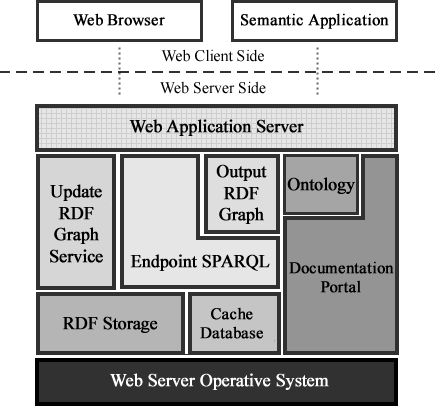
\includegraphics[width=10cm]{images/phd/infrastructure}
\caption{Infraestructra \linkeddata propuesta en la Biblioteca del Congreso de Chile.}
\label{fig:bcn-infraestructura}
\end{figure}

También, hay que destacar el proceso de adopción definido en este enfoque, ver Figura~\ref{fig:bcn-proceso}, en el cual
quedan recogidos los pasos para promocionar las bases de datos legislativas utilizando datos enlazados. Este proceso
es similar al propuesto por el \gls{W3C}, ver Sección~\ref{linked-data-cookbook}, y ciclo de vida definido en el proyecto LOD2, ver Figura~\ref{fig:lod-lifecycle}, 
difiere en el nombrado de los procesos y las herramientas a utilizar en cada una de las fases.

\begin{figure}[!htb]
\centering
	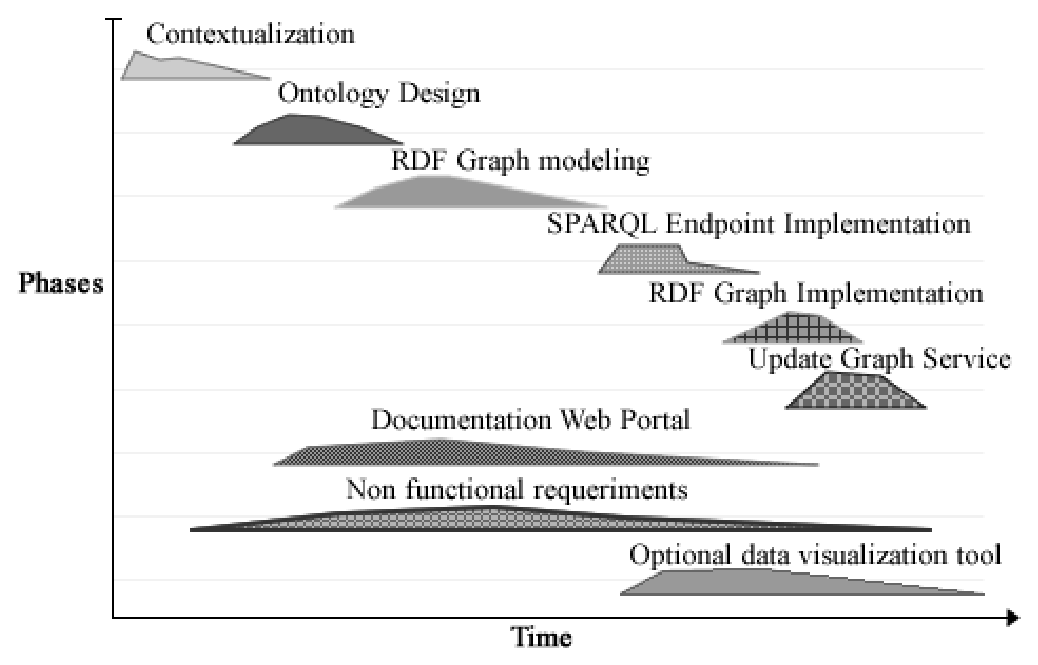
\includegraphics[width=10cm]{images/phd/process}
\caption{Proceso de implantación de \linkeddata en la Biblioteca del Congreso de Chile.}
\label{fig:bcn-proceso}
\end{figure}


\subsubsection{\textit{Talis Platform}}
En este caso la plataforma Talis~\cite{talis} es un servicio o producto que sirve para la creación de una
infraestructura de \linkeddata en la nube. Ha tenido un gran éxito ya que sus creadores son grandes
impulsores de la iniciativa (por ejemplo son los autores de ``Linked Data Patterns'') y han trabajado
en casos de enorme repercusión, como la apertura de datos públicos del Gobierno del Reino Unido. Ofrecen 
 una ``suite'' de herramientas y servicios para cumplir las directrices de \linkeddata, teniendo en cuenta 
la mayor parte de la casuística presente en la producción, publicación y consumo de datos enlazados. En resumen, se provee una plataforma
que cubre toda la cadena de valor de los datos enlazados y cumple todas las directrices necesarias.

Entre las características más llamativas que ofrecen dentro de esta plataforma se encuentran las
siguientes (extraídas de la propia página web de Talis):

\begin{itemize}
    \item \textit{A simple, consistent web API for storing, managing and retrieving both structured and unstructured data.}
    \item \textit{Flexible, schema-free metadata that allows applications to be easily evolved.}
    \item \textit{A range of data access and query options enabling easy integration into both new and existing applications.}
    \item \textit{Access control options to support hosting of both public and private data.}
    \item \textit{A data hosting solution that is founded on open internet standards and web architectural best practices.}
    \item \textit{Software as a Service, enabling rapid development with zero deployment costs.}
    \item \textit{Low, even free, utility based pricing for services and hosting allowing costs to grow with usage.}
    \item \textit{A highly available and scalable infrastructure to ensure that the repository grows in line with your applications needs.}
\end{itemize}

Evidentemente este tipo de soluciones son de extraordinario interés para las Administraciones Públicas, ya que consiguen
un producto llave en mano con todas las capacidades necesarias para disponer de una infraestructura de datos
enlazados de última generación. Es interesante destacar esta plataforma por dos motivos principales: sus creadores
son relevantes desde un punto de vista científico y han realizado una gran transferencia tecnológica desde
el campo de la investigación al industrial.

En la misma línea de la plataforma Talis podemos encontrar otras empresas que ofrecen productos y herramientas
de alto valor como son Virtuoso de OpenLink o ToqQuadrant. Todos ellos son miembros activos en la comunidad
de \linkeddata y están presentes en los principales grupos de trabajo de esta iniciativa en el \gls{W3C}.
 
\subsubsection{\textit{Linked Open Data: The Essentials}}\label{linked-data-spec}
Este libro~\cite{Bauer2012} realizado en colaboración entre \gls{REEEP} (\textit{Renewable Energy and Energy Efficiency Partnership}) y la compañía \textit{Semantic Web}
es un manual que da respuesta a algunas de las preguntas comunes que surgen en el despliegue de una infraestructura de datos enlazados
en el seno de una organización. En general, se trata de una recopilación de las buenas prácticas que se han revisado
en los anteriores apartados y que focaliza en los beneficios de la publicación de datos enlazados para las
organizaciones. La parte más destacada de este libro, ver Figura~\ref{fig:lod-essentials}, se centra en la descripción de las tareas
a realizar y de los posibles servicios haciendo hincapié en las tareas de publicación y consumo de datos enlazados.

\begin{figure}[!htb]
\centering
	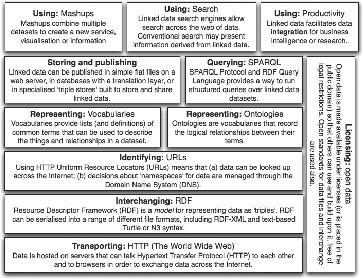
\includegraphics[width=10cm]{images/phd/lod-essentials}
\caption{\textit{Elementos of the Linked Open Data Puzzle}.}
\label{fig:lod-essentials}
\end{figure}


\subsubsection{Documentación específica}\label{linked-data-spec}
Desde distintas organizaciones tales como Administraciones Públicas y Universidades,
así como personalidades relevantes en esta materia se ha promovido la realización de proyectos, guías y artículos que tratan diversos aspectos
relacionados con la iniciativa de \linkeddata. Todos ellos tratan de aportar nuevos enfoques, herramientas y documentación
a los distintos procesos implicados en el despliegue de esta iniciativa, entre los que podemos destacar:

\begin{itemize}
 \item ``\textit{A Proposal for Governmental Data URIs}'' realizado por Gregory Todd Williams, Tim Lebo y Alvaro Graves.  % http://iw.rpi.edu/wiki/A_Proposal_for_Governmental_Data_URIs
 \item ``\textit{Designing \gls{URI} Sets for the UK Public Sector}''~\cite{uris-uk} realizado por ``The Cabinet Office'' del Reino Unido. 
 \item ``\textit{Federal Information Security Management Act (FISMA)}'' proyecto realizado por  el ``National Institute of Standards and Technology'' de Estados Unidos.
 \item La documentación disponible en la Biblioteca del Congreso de Estados Unidos.
 \item Los artículos de Jeni Tennison sobre distintos aspectos relativos al diseño de URIs, etc.
 \item El \textit{framework} SERIMI~\cite{Serimi} de reconciliación de entidades.
 \item Los documentos y software elaborados por la empresa Epimorphics.
 \item Las guías de datos abiertos y enlazados de las distintas Administraciones Públicas, tanto a nivel estatal 
España, Reino Unido, Francia, Alemania, etc., como a nivel regional, Asturias, País Vasco o Cataluña o incluso local como
en el Ayuntamiento de Zaragoza.
\end{itemize}

En general se trata de documentos o herramientas que nacen de la necesidad y experiencia en la resolución de ciertos
 problemas relacionados con la apertura de datos y su enlazado, que se reproducen en cada escenario en el cual se
aplica esta iniciativa. Todo este trabajo y esfuerzo supone un gran valor para la comunidad de desarrolladores
y de personas implicadas en aplicar estos principios.

\subsection{Escenarios y Casos de Uso de Éxito}
La irrupción de la corriente de \linkeddata ha conllevado la realización práctica y real de una parte de la denostada Web
Semántica. Muchas son las instituciones, administraciones públicas,
empresas privadas, universidades, hospitales, que bajo esta corriente están
liberando sus datos en el entorno web siguiendo las directrices  marcadas por
Tim Berners-Lee. El principal objetivo consiste en la apertura de datos, para que
una vez publicados sirvan como fuente para la creación de aplicaciones agregando
distintos recursos (\textit{mashups}), facilitando la transparencia de comportamiento en
ciertos organismos, suministrando servicios de valor añadido basados en el contexto
del usuario o simplemente desde un punto de vista de tendencia, para obtener
presencia en la nueva \wod. 

No obstante, este nuevo enfoque conlleva varios desafíos a nivel científico que están siendo
abordados actualmente, tales como el procesamiento de grandes cantidades de
datos de forma eficiente, gestión-formalización-explotación del conocimiento
subyacente mediante reglas, razonamiento distribuido, \textit{stream-reasoning}, \textit{real
time linked data}, \textit{complex event processing}, reconciliación de entidades,
visualización etc., los casos de uso de aplicación de estas investigaciones representan un abanico muy amplio: recomendación de recursos
(películas, libros, etc.), análisis de sentimientos y opiniones, domótica,
\textit{smart-cities}, computación ubicua, \textit{green computing}, sistemas de soporte a la
decisión en campos como \textit{e-Health}, etc.

Hasta el momento esta iniciativa ha estado muy ligada al mundo técnico, es decir, tanto la publicación como el 
consumo de los datos estaba muy orientado a un perfil fundamentalmente técnico. No obstante, al igual que con la web que hoy conocemos, 
la \wod todavía no trascendido al gran público, es por ello que surgen varios desafíos~\cite{DBLP:journals/semweb/DadzieR11} para conseguir que el despegue definitivo 
de esta corriente:

\begin{enumerate}
 \item Necesidad de una capa de presentación. Si una persona buscara cierto recurso 
 que tiene definido según unas necesidades, la expresión de esta consulta implicaría características de 
sistemas de \textit{Information Retrieval} o tareas de análisis de sentimientos. Más en concreto: a) descubrimiento de qué fuentes pueden tener 
disponible esa información; b) validación y cooperación entre las distintas fuentes de datos disponibles; c) consulta a 
las fuentes de datos seleccionadas y d) análisis, presentación y manejo de las vistas de los resultados. En este sentido, la tendencia actual 
reside en ``ocultar'' la existencia de varios datasets detrás de los sistemas de búsqueda, así como la consulta y manejo de los 
resultados, de tal manera que el usuario no es consciente de las oportunidades de explotación de datos de las que podría disponer. 
Es necesario aclarar que el conocimiento de la tecnología no debe ser la clave para la explotación de la misma por el usuario 
final, pero si que es necesario proveer los métodos y herramientas adecuadas para que el usuario obtenga el máximo partido de 
la información subyacente. De esta manera si la tendencia de \linkeddata supone una revolución respecto a la actual web de documentos, se 
deberían proveer nuevos mecanismos de acceso a la información y no restringirse a los tradicionales modelos de interacción con el 
usuario (por ejemplo un formulario de búsqueda). 
\item Combinación efectiva de los distintos \datasets. Teniendo en cuenta que existe un catálogo de datos y 
  vocabularios en constante crecimiento, es necesario proveer los mecanismos necesarios (alineación, \textit{mapeo} y fusión) para que 
la combinación de los mismos sea eficiente en el sentido de que la identificación de recursos similares, el 
encaje mediante propiedades o la mezcla de recursos sea intuitiva, tanto desde un punto de vista técnico como del usuario final. 
Las técnicas que permiten llevar a cabo este desafío no son deterministas y en muchos casos se basan en algoritmos que chequean 
la estructura de los recursos o bien realizan comparaciones basadas en procesamiento del lenguaje natural entre las descripciones de los recursos.
\end{enumerate}

En el contexto de \linkeddata surgen dos principales vías de actuación sobre los datos: publicación y consumo, concretamente en el campo de consumo de 
datos surgen varios interrogantes como:
\begin{itemize}
\item Gestión de datos a nivel web.
\item Procesamiento de consultas federadas~\cite{sparqlOpt}.
\item Búsqueda.
\item Descubrimiento de \datasets y recursos: URIs, datos adicionales o datasets relevantes para una consulta.
\item \textit{Datasets} evolutivos: cómo afectan los cambios en los datasets a las consultas, monitorización.
\item Razonamiento e inferencia de conocimiento en la \wod.
\item Calidad de los datos: evaluación de la calidad de la información, confianza y \textit{provenance}.
\item Interfaz de Usuario para la interacción con la \wod: interacción y usabilidad, visualización, interfaces basadas en lenguaje natural.
\end{itemize}


Por otra parte, en las Administraciones Públicas se está trabajando exhaustivamente en el campo de la reutilización de datos, en la actualidad 
se pueden señalar algunos ejemplos:
\begin{itemize}
\item Gestión de bibliotecas digitales, la Biblioteca del Congreso de Chile o del Congreso de Estados Unidos.
\item Gestión de flotas. Aplicación del Ayuntamiento de Gijón para el control de la línea urbana de autobuses .
\item Sistemas de búsqueda y recomendación basadas en perfiles usuario enlazados.
\item Sistemas de e-Health. Para el soporte a la decisión en el diagnóstico.
\item Sistemas de Información Geográfica. GIS+Linked Data.
\item Gestión y publicación de información financiera.
\item Otros múltiples campos de actuación: Turismo, Tráfico, Educación, Domótica, \textit{Semantic Sensors}, etc.
\end{itemize}

En último término todas las iniciativas basadas en \linkeddata convergen al objetivo principal de la misma:
\begin{Frame}
\textit{Linked Data is about using the Web to connect related data that wasn't previously linked, or using the Web to lower the barriers 
to linking data currently linked using other methods.} 
\end{Frame}


Teniendo en cuenta el valor añadido de la visualización de datos para Linked Data,
 se pueden establecer una serie de requisitos~\cite{journals/semweb/DadzieR11} a cumplir, que actualmente están parcialmente cubiertos 
por algunas herramientas, no obstante, se puede establecer una guía de características necesarias para el manejo de datos enlazados y su 
visualización, siendo uno de los grandes elementos de investigación actual.
\begin{itemize}
 \item Requisitos de alto nivel: a) capacidad para generar vistas agregadas de los datos; b) soporte para la creación de filtros y c) soporte para 
la visualización detallada de los recursos.
\item  Requisitos de consumo de datos: a) manejo de datos multidimensionales; b) manejo de datos jerárquicos;
c) generación de estructuras de representación: grafos, árboles, etc.; d) identificación de las relaciones significativas en los datos;
e) extracción de datos y nuevas relaciones y f) contextualización de usuario y multidispositivo.
\item Requisitos directamente relacionados con \linkeddata: a) navegación entre los distintos datasets; b) exploración de los datos 
para obtener consciencia de la estructura y de las relaciones; c) exploración que permita análisis con el objetivo de identificar incoherencias, etc.;
d) consulta transversal a través de los distintos datasets mediante un lenguaje formal y e) capacidad para extraer partes de los datos para su posterior reutilización.
\item Requisitos relacionados con la navegación semántica: a) navegación facetada y contextualizada del usuario; b) exploración del conocimiento, inferencia, etc.;
c) consulta avanzada con filtros de lenguaje natural; d) análisis detallado y explicación de las inferencias y e) presentación de resultados de análisis.
\end{itemize}





\chapter{\label{capitulo:eproc-sm}Tendencias actuales en Semántica} 
El creciente uso de Internet durante los últimos años ha puesto de manifiesto un
nuevo entorno de ejecución para las aplicaciones, utilizando como nueva
plataforma la web, el gran sistema distribuido. Nuevas tecnologías y paradigmas
están emergiendo para dar soporte al desarrollo y despliegue de aplicaciones y
servicios, así como para la publicación de datos e información. Los modelos de
desarrollo están cambiando a un estilo más colaborativo en el cual las empresas
ofrecen su software como servicios (\textit{Software as a Service}-\gls{SaaS}) materializado a
través del paradigma de \textit{cloud computing}~\cite{Armbrust09abovethe}, implementado con tecnología de
servicios con el objetivo de que terceros puedan utilizar estos servicios para
la construcción de aplicaciones agregadas con valor añadido. 

En este sentido, tal como se ha señalado, iniciativas como la Web Semántica, que a través de modelos y
formatos de datos de conocimiento compartido unificados, intentan elevar el
significado de los elementos y recursos que están disponibles en la web, con el
objetivo de mejorar la integración e interoperabilidad entre aplicaciones, están 
impulsando la implantación de este enfoque. Dentro de la iniciativa de Web
Semántica hay que destacar dos esfuerzos: 
\begin{enumerate}
 \item La iniciativa \linkeddata que tal y como se ha descrito propone la publicación de datos
enlazados siguiendo el modelo \gls{RDF} para facilitar la creación de una web de
datos en la que éstos se puedan mostrar, intercambiar y conectar a través de
URIs. La tendencia actual de publicación de datos enlazados está marcando una
evolución en la interoperabilidad de aplicaciones, con el consiguiente efecto que
conlleva para las relaciones \gls{B2B}, \gls{B2C} o \gls{A2A}. Entre los casos de éxito
podrían destacarse: administración electrónica (iniciativa de \textit{Open Government
Data}, contratación pública de bienes y servicios (\eproc), oferta formacional , contextualización de aplicaciones, \textit{mashups},
etc. 

\item El desarrollo de lenguajes y formalismos lógicos para representar el conocimiento sobre un universo de discurso, permitiendo la inferencia de nuevos
datos a partir de los datos ya publicados. En este contexto se ha impulsado nuevamente el uso de las técnicas de razonamiento y de sistemas basados en conocimiento, como 
las ontologías y los sistemas basados en reglas (Ontobroker, XSB, etc.) o de producción (Drools , JRules , etc.). 
La aplicación de estos sistemas está ampliamente asentada en la resolución de diversos problemas
(diagnóstico, planificación, reglas de negocio, etc.) pero siempre utilizando un enfoque para la representación del conocimiento y de los datos, en muchos casos
específico y no estandarizado. Por tanto, debe tenerse en cuenta la flexibilidad, tanto para la integración como para la interoperabilidad de las aplicaciones. Una arquitectura orientada a
servicios sobre la plataforma web, utilizando los protocolos actuales y que se beneficie de las iniciativas relativas a la Web Semántica puede dar respuesta a
este punto clave. La implantación de un sistema basado en conocimiento, concretamente de
sistemas basados en reglas y de razonamiento, que hagan uso de una infraestructura estandarizada y cooperativa redunda en gran beneficio para la
resolución de problemas basados en conocimiento declarativo y compartido, mejorando tanto la independencia tecnológica de las aplicaciones como la experiencia de usuario.
\end{enumerate}


Al amparo de la visión de la Web Semántica, el \gls{W3C} ha promovido la creación de varias recomendaciones que intentan ofrecer soluciones 
para las diferentes capas de la arquitectura. En concreto, RDF es el lenguaje de representación básico que 
permite representar tripletas de la forma sujeto-predicado-objeto. Dichas tripletas 
forman un grafo dirigido que puede integrarse automáticamente con otros grafos obtenidos de otros servidores. 
Otra de las tecnologías propuestas por el W3C es RDFS, que permite la definición de clases, propiedades e individuos y 
ofrece unos mecanismos básicos de inferencia mediante reglas. RDFS facilita la creación e integración de vocabularios 
pero carece de expresividad suficiente para describir relaciones avanzadas como complementos de conjuntos o cardinalidades. Las limitaciones 
expresivas de RDFS propiciaron la definición de \gls{OWL}, un lenguaje de definición de ontologías basado en lógica descriptiva. 
La versión 2 de OWL llegó a status de recomendación del W3C en octubre del año 2009. Una de las principales mejoras de esta versión, estaba 
encaminada a la resolución del compromiso entre la expresividad y la complejidad de los razonamientos, mediante la definición de perfiles o 
fragmentos computacionales. Los tres perfiles de OWL2: EL, QL y RL, son sublenguajes del mismo que permiten alcanzar una complejidad 
polinómica para tareas de razonamiento estándar limitando la expresividad. La combinación de OWL con lenguajes basados en 
reglas que incluyen la negación, como los \textit{dl-programs}~\cite{DBLP:conf/rr/Motik08} han sido desarrollados en las redes de excelencia 
\textit{REWERSE} y \textit{Knowledge web} y definen la interoperabilidad entre las reglas y las ontologías. 

El problema del intercambio de reglas entre los distintos sistemas de razonamiento e inferencia también ha sido abordado recientemente, 
así encontramos la recomendación del W3C RIF de 22 de junio del año 2010. 
\gls{RIF} es, de nuevo, una familia de lenguajes (\textit{Core},\textit{Production Rule Dialect, BLD Basic Logic Dialect, Datatypes and Built-Ins, Framework for Logic Dialects}, etc.) 
con diferente expresividad, cuyo objetivo es convertirse en \textit{lingua franca} para el intercambio de conocimiento basado en reglas en la web. 
El formato utilizado por RIF es \gls{XML} y su combinación con ontologías permite que las reglas y el modelo de datos sobre los que se van a aplicar 
las reglas se pueden intercambiar entre distintos actores. Para interpretar RIF es necesario realizar una traducción desde este vocabulario al motor de inferencia
deseado. En el ámbito de intercambio de reglas hay que resaltar el antecesor de RIF, RuleML que es una iniciativa internacional sin ánimo de lucro, que cubre
los aspectos del intercambio y la interoperabilidad de reglas. Esta iniciativa mantiene una estrecha relación con los grupos de OASIS en reglas, así como con
ISO Common Logic (estándar en el año 2007). RuleML, como grupo, también contribuye en \gls{OMG} a \gls{SBVR}, específicamente en el apartado de \textit{Production Rule Representation} (PRR) cuya última
versión data de diciembre del año 2009.

Para la consulta de datos \gls{RDF} se ha desarrollado \gls{SPARQL}, un lenguaje de consulta y un
protocolo de acceso que permiten definir un terminal (o \textit{endpoint}) en el que se publican conjuntos de datos (o \textit{datasets}) RDF y 
que están disponibles como servicios en la web. Actualmente se está trabajando en vocabularios para
definir datasets y poder enlazarlos entre sí de forma sencilla. Con el uso de
SPARQL han aparecido propuestas para la definición de reglas de producción con
este lenguaje (extensión \textit{SPARQL with Updates-\gls{SPARUL})} de modo que se ejecuten
directamente sobre una base de datos en RDF, como puede ser SPARQL-Rules~\cite{citeulike:1294570},
también existen enfoques para la consulta de ontologías OWL con SPARQL~\cite{Sirin07sparql-dl:sparql} y
en la especificación que se elabora actualmente, SPARQL 1.1, se
dispone de un vocabulario para definir los servicios disponibles. Finalmente y
con el objetivo de personalizar la vista de las aplicaciones por el usuario y su
contextualización se ha aplicado el uso de reglas en formato \gls{JSON}~\cite{conf/ki/GiurcaP08}. 


La evolución de los formalismos para definir ontologías lleva emparejado el
desarrollo de razonadores que puedan llevar a cabo las inferencias necesarias.
Desde el pionero KL-ONE hasta este momento, se han implementado múltiples
razonadores basados en lógica descriptiva siguiendo diferentes técnicas. En la
actualidad, se pueden destacar Fact++~\cite{Tsarkov2006}, Pellet~\cite{Sirin_Parsia_Grau_Kalyanpur_Katz_2007} y RacerPro~\cite{Rajeev2001Racer}
que se basan en la técnica conocida como \textit{semantic tableaux}. A pesar de las altas
complejidades, en el caso peor los algoritmos de razonamiento utilizados en estos sistemas son capaces de resolver muchas tareas prácticas gracias al uso de
diversas optimizaciones. Para resolver dichas limitaciones, especialmente, al
tratar con grandes cantidades de datos, se han buscado técnicas alternativas
como el algoritmo de resolución utilizado en KAON2~\cite{journals/ercim/Motik08}, el sistema
\textit{hipertableau} empleado en HermiT~\cite{msh09hypertableau}, las técnicas de eliminación de tipos~\cite{DBLP:conf/aaai/RudolphKH08}
 o las recientes técnicas basadas en eliminación de consecuentes~\cite{DBLP:conf/ijcai/SimancikKH11}.

La utilización de reglas se ha propuesto como una alternativa para la
implementación de razonadores. En este caso, las definiciones de la ontología
son compiladas a un conjunto de reglas, que se aplica al conjunto de datos para obtener las inferencias correspondientes. La principal
ventaja de estos razonadores es que se basan en técnicas ya conocidas en el
ámbito de la programación lógica con diversas implementaciones disponibles, constituye sin embargo una
desventaja, que generalmente es necesario utilizar subconjuntos de \gls{OWL}, como el
conocido OWL Horst~\cite{Horst2005}. Uno de los mayores retos de la Web Semántica es la búsqueda de técnicas que
mejoren la escalabilidad de los razonadores, en esta línea, han surgido
trabajos que proponen la utilización de tecnologías distribuidas para afrontar
dicha complejidad. Por ejemplo, en~\cite{SomaPrasanna2008}
se propone la implementación de un sistema de inferencia paralelizable sobre OWL
Horst, mediante un particionado de las reglas. Con el objetivo de mejorar la
escalabilidad, en~\cite{springerlink:10.1007/978-3-642-04930-9_43} se propone un algoritmo para realizar inferencias sobre
RDFS que se aplica a un \textit{benchmark} de $10.000$ tripletas, proponiendo como trabajo futuro la posible aplicación de MapReduce~\cite{citeulike:430834,DBLP:conf/semweb/UrbaniKOH09}. En~\cite{UrbaniMaassenBal2010} se describe una implementación basada en el algoritmo MapReduce
logrando realizar el cierre parcial de $864$ millones de tripletas en RDFS, en una
hora utilizando 32 procesadores. Recientemente, los mismos autores
desarrollaron el sistema WebPIE~\cite{Urbani2010WebPIE}, el cual ha sido capaz de
realizar inferencias sobre $1$ billón y medio de tripletas, en $6,1$ horas utilizando
$32$ nodos, mediante reglas de OWL Horst. El sistema SAOR se ha implementado para
dar soporte al buscador semántico SWSE, incorporando un razonador sobre OWL
Horst~\cite{HoganHarthPolleres2009}, dicho sistema ha diseñado un nuevo algoritmo
distribuido, mejorando la escalabilidad de la implementación~\cite{DBLP:conf/semweb/HoganPPD10}. Finalmente, también se está 
trabajando~\cite{HausenblasCloudLOD} en la conjunción de \linkeddata y \textit{cloud computing} para el procesamiento de grandes cantidades de datos.


\chapter{\label{capitulo:eproc-sm}\textit{e-Procurement} y Semántica} 
La construcción de un modelo semántico sobre un dominio de negocio concreto
consiste en el desarrollo de un sistema de conocimiento que describa las
entidades y propiedades, así como las relaciones lógicas que existen entre
las mismas. Un aspecto, muchas veces minusvalorado, es que en estos modelos de
dominio es necesario describir también los procesos, las restricciones y en
general, los aspectos dinámicos del dominio. Este tipo de modelos formalizados
mediante un lenguaje lógico, como ya se ha descrito, se denominan ``ontologías''. La selección de la lógica apropiada para la modelización de 
la base de conocimiento no es una cuestión sencilla y se deberán contemplar diferentes
factores tales como grado de computabilidad, decidibilidad, soporte razonadores, etc. Existen
diferentes vocabularios y lenguajes que permiten modelar un cierto dominio, algunos
de los cuales ya se han repasado (\gls{RDF}, RDFS, \gls{OWL} y \gls{WSML}) en la Sección~\ref{sect:arch-ws}, no obstante, existen otros estrechamente
ligados a entornos de negocio, que a continuación se presentan.


\begin{description}
\item[\gls{RIF} (\textit{Rule Interchange Format})~\cite{rif-core}.] RIF constituye una familia de lenguajes con diferente expresividad, 
cuyo objetivo es convertirse en \textit{lingua franca} para el intercambio de
conocimiento basado en reglas en la Web. Define la compatibilidad con
documentos RDF y OWL, además está especialmente diseñado para integrarse con
sistemas de inferencia basados tanto en reglas de producción, como de
Programación Lógica. La ventaja de RIF respecto de OWL es una mayor expresividad, 
que permite expresar conocimiento causal y procedimental. 


\item [\gls{SCOR} Model (\textit{Supply-Chain Operations Reference-Model}).] Es un modelo conceptual de
referencia para la especificación y formalización de los procesos de negocio
asociados a las cadenas de suministro. Este modelo define los procesos de
planificación, fabricación, entrega, evolución e inventarios de productos en una
cadena logística.

\item [\gls{SBVR} (\textit{Semantics of Business Vocabulary and Business Rules}).] Es un estándar
(ISO 704/1087) desarrollado por el \textit{Object Management Group} (\gls{OMG}). Define un
metamodelo para el desarrollo de modelos semánticos de vocabularios y reglas de
negocio. La idea es que a partir del lenguaje natural se puedan expresar
vocabularios y reglas de negocio en un dominio concreto. La construcción de un
modelo de negocio mediante el SBVR recoge el vocabulario de conceptos del
dominio y la definición de lógica formal asociada.

\item [Clasificaciones de productos de comercio electrónico~\cite{Leukel-ecatalog2005,Leukel-standard,Leukel-automating}.] Para
facilitar el intercambio automático de información y la anotación de los diferentes productos
y documentos que forman parte del comercio electrónico, distintos sectores de
actividad económica han desarrollado sus propias terminologías o
vocabularios~\cite{Norbert-class} controlados, para armonizar mediante códigos unívocos la identificación de
los objetos de negocio. Ejemplos de estos vocabularios son: el estándar eCl@ss o
la clasificación \gls{UNSPSC} entre otros, ver Sección~\ref{sect:pscs}.


\item [\gls{ebXML} (\textit{Electronic Business using eXtensible Markup Language}).] Es un lenguaje
\gls{XML} elaborado por \gls{OASIS} y UN/CEFACT, también consta de una infraestructura que permite la comunicación entre entidades
participantes en transacciones de negocio electrónico, favoreciendo la interoperabilidad y la seguridad de una forma homogénea entre las distintas partes.
La propuesta original cubría cinco capas: \textit{Business processes}; \textit{Collaboration protocol agreements};
\textit{Core data components}; \textit{Messaging} y \textit{Registries and repositories}.

eBXML ha sido aprobado por \gls{ISO} en un conjunto de especificaciones, ISO 15000:  ISO 15000-1: ebXML \textit{Collaborative Partner Profile Agreement};
ISO 15000-2: ebXML \textit{Messaging Service Specification}; ISO 15000-3: \textit{ebXML Registry Information Model}; ISO 15000-4: ebXML \textit{Registry Services Specification};
y ISO 15000-5: ebXML \textit{Core Components Technical Specification}, Version 2.01.

\item [\gls{XBRL} (\textit{extensible Business Reporting Language}).] 
Es una norma elaborada en el año 1998 por Charles Hoffman, contable y auditor, para
simplificar la automatización del intercambio de información financiera mediante
el uso del lenguaje XML. La familia de lenguajes XBRL se ha realizado para
satisfacer las exigencias principalmente de información financiera y
empresarial, permite aplicar etiquetas identificativas multilenguaje con
significado, por ejemplo indicando si es un valor monetario, también es posible
mostrar la relación que guardan los elementos entre sí, así se podría saber cómo se
calculan. Una característica muy importante es la capacidad de extensión, de
esta forma es capaz de adaptarse para casos particulares de empresas. 

\end{description}

\subsection{Actividades de aplicación de Semántica en \textit{e-Procurement}}
Desde la creación del movimiento de la Web Semántica, en concreto de la realización
práctica mediante \linkeddata, se han aplicado los principios de estas iniciativas a múltiples
dominios como ya se ha reseñado en las secciones anteriores. Evidentemente en un sector como 
la Administración Pública, caracterizado por su amplitud, casuística y carácter estratégico para todos los ciudadanos
es por lo que la semántica y sobre todo las corrientes de \opendata y \linkeddata han penetrado con mucha fuerza en los últimos años. 
En un principio los esfuerzos como en otros dominios, se centraban en el modelado de la administración
como organización y de sus procesos, con el objetivo de mejorar la interoperabilidad e integración
entre las aplicaciones y facilitar los trámites burocráticos. En muchos casos se han desplegado
soluciones flexibles basadas en la reutilización de información, procesos y conocimiento a través
de grandes bases de datos compartidas, servicios web y sistemas basados en reglas, no obstante la inmersión
de la semántica propiamente dicha se centraba en la realización de modelos para formalizar
cuestiones relativas a documentación y a procesos administrativos. Por ello,
la irrupción de \opendata y \linkeddata ha reorientado el esfuerzo de las Administraciones Públicas
para aprovechar la semántica en su beneficio. 

Por otra parte, también han surgido iniciativas~\cite{DBLP:journals/tcci/Alor-HernandezAJPRMBG10} relacionadas con \eproc, pero desde un punto de vista
de las cadenas de suministro, en las cuales se modelan de forma completa un entorno de proveedores y suministros mediante la coordinación
de los recursos software, hardware y humanos propios de un entorno de este tipo, como son \gls{ERP}s, robots o las propias personas. 

\subsubsection{Ontología de Contratos Públicos del proyecto LOTED}
El diseño de la ontología en el proyecto LOTED~\cite{loted-project}, es de suma importancia debido a su consideración 
como primer gran esfuerzo por aunar las iniciativas de \linkeddata y \opendata en el campo de la contratación 
pública electrónica. En este proyecto la propuesta principal consiste en la transformación directa 
de la información proveniente del \gls{RSS} de \gls{TED} a \gls{RDF} para su posterior indexado en un repositorio y acceso 
mediante un \textit{endpoint} de \gls{SPARQL}. Como sucede un muchos casos relacionados con la iniciativa 
de \linkeddata la ontología realizada, ver Figura~\ref{fig:public-contracts-ontology-loted}, está orientada a la representación de los datos en sí, estableciendo 
un modelo formal en el cual enclavar los recursos RDF generados, pero si bien este enfoque es válido, tan sólo 
representa una parte de la casuística presente en el dominio de la contratación pública electrónica. El intento 
realizado en TED se centra en el diseño de las entidades presentes en la información del RSS para así suministrar 
un modelo formal a los recursos RDF. Por todo ello, esta ontología sirve como una gran fuente de información 
para comprobar que tipo de entidades se recogen o publican en el RSS de TED, pero en un espectro más amplio 
se considera insuficiente para la representación de información teniendo en cuenta los modelos de datos 
disponibles en las plataformas de contratación o el propio de \gls{opXML} realizado en el proyecto ``10ders Information 
Services'', como ha quedado señalado en la Sección~\ref{data-model-eproc}. 

Por otra lado y desde el punto de vista del acceso a los datos, se ofrece la posibilidad de la realización 
de consultas en SPARQL seleccionando una serie de códigos y acotando los resultados por fechas, sin embargo este sistema 
parece desactualizado y no se han realizado cambios en los últimos dos años. 

\begin{figure}[h]
 \centering
    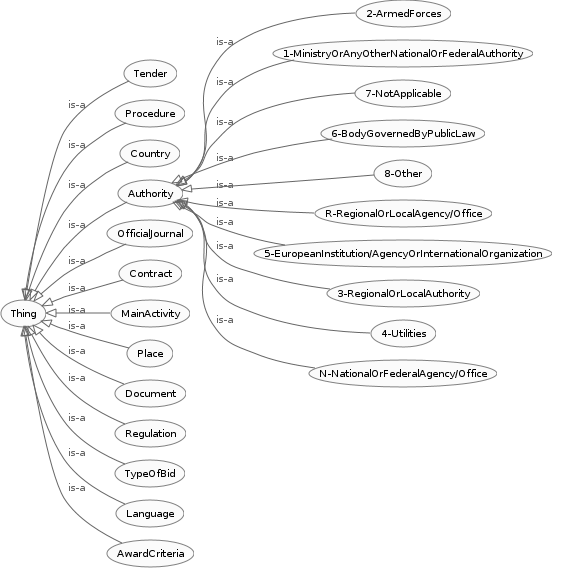
\includegraphics[width=14cm]{images/phd/loted-ontology}
  \caption{Ontología de Contratos Públicos del proyecto LOTED.}
 \label{fig:public-contracts-ontology-loted}
\end{figure}

\subsubsection{Ontología de Contratos Públicos de la República Checa}
Esta ontología está siendo desarrollada por el grupo \textit{Knowledge Engineering Group} 
de la \textit{Charles University} de Praga en la República Checa. Parte del esfuerzo está siendo
cubierto parcialmente dentro del proyecto europeo LOD2 en su paquete de trabajo \textit{WP9A – LOD2 for a Distributed Marketplace for Public Sector Contracts}, cuya descripción es la siguiente:

\begin{Frame}
\textit{The objective of this use case is to explore and demonstrate the application of linked data principles for procuring contracts in the public sector...}
\end{Frame}

Este trabajo enlaza perfectamente con el propósito de este documento, esto es cubrir el sector de los contratos
públicos con semántica y concretamente con la iniciativa \linkeddata. Es por ello que se ha establecido
contacto con los integrantes del grupo de investigación de esta Universidad para aprovechar y realimentar
esfuerzos, como fruto de esta colaboración han empezado a reutilizar los códigos CPV, resultado de este trabajo y del proyecto ``10ders Information Services''.

La ontología que se ha desarrollado en este grupo, ver Figura~\ref{fig:public-contracts-ontology}, tiene como intención recoger
la información y datos de los contratos públicos de forma estructurada, para que pueda ser consumida
automáticamente tanto por personas como por máquinas, desarrollándose también dentro del ámbito
de la iniciativa de \opendata de la República Checa. Desde un punto de vista del diseño reutiliza varios
vocabularios y ontologías ya disponibles, como \textit{Payments Ontology} del Reino Unido, lo que confiere a este modelo un carácter integrador y 
reutilizable. No obstante, abordar la descripción de toda la casuística del proceso de contratación pública electrónica parece
muy ambicioso y podría presentar problemas de interoperabilidad, integración y reutilización ya que 
puede estar muy orientada a la problemática de un entorno particular. Otro de los puntos importantes
que se deben abordar, y parcialmente recogidos en esta ontología y que deben servir de guía, están referidos a 
la adición de metainformación para \textit{provenance}, licencia, etc., que si bien en algunos
\datasets es importante, en la información de carácter público es fundamental y debe ser un requisito
para las propias entidades públicas.

\begin{figure}[h]
 \centering
    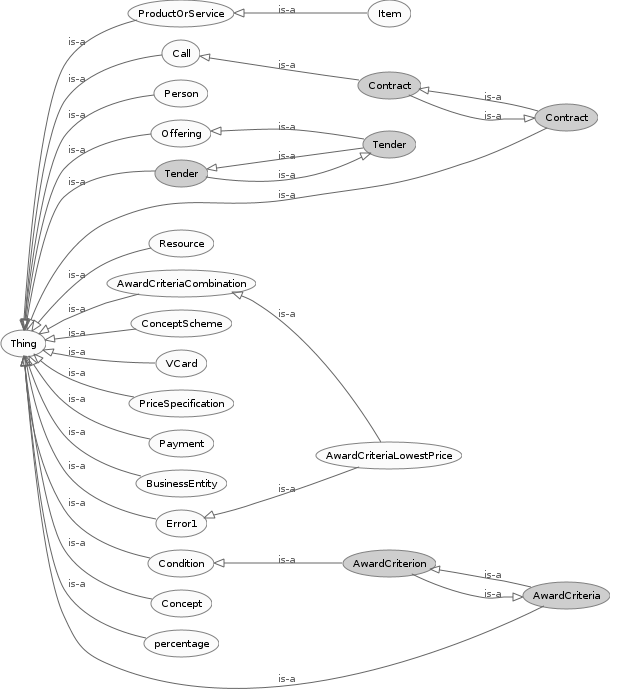
\includegraphics[width=14cm]{images/phd/public-contracts-ontology}
  \caption{\textit{Public Contracts Ontology from Czech Republic.}}
 \label{fig:public-contracts-ontology}
\end{figure}


\subsubsection{Clasificaciones Estándar de Productos}\label{semantica:pscs}
Las clasificaciones de productos, son instrumentos claves de estandarización~\cite{Leukel-standard} que nacen con el fin de
conseguir una clasificación común de productos y servicios. En general, son variadas~\cite{Leukel-ecatalog2005}
y obedecen a intereses particulares dependiendo del sector como e@Class o RossetaNET,
o bien de carácter global como \gls{UNSPSC} u otras destinadas a un dominio particular como el \gls{CPV} en la Administración Pública, ver Sección~\ref{sect:pscs}. Las diferencias
estriban en su alcance y cobertura sectorial, pero también en el grado de especificidad o nivel
de profundidad que existe para describir los productos o servicios.

Como señala Hepp\cite{HeppTrueComplexity,HeppEclass,HeppMethodology} todos estos
estándares reflejan una combinación de componentes variables, que pueden ser
utilizados para la construcción de una ontología derivada a partir de la clasificación.
Sin embargo, se puede identificar una estructura común subyacente a todas ellas y
que es fundamental señalar para proporcionar un modelo de datos semántico universal para este tipo de clasificaciones, consistente 
en que todas estas clasificaciones se ordenan jerárquicamente. 

\begin{description}
 \item [Categorías de productos.] Las clasificaciones se dividen en categorías o
clases de productos, agrupando los distintos elementos del catálogo.
\begin{itemize}
 \item Las categorías de la clasificación se organizan jerárquicamente.
 \item Cada elemento de la clasificación pertenece a una categoría de
productos.
 \item Cada elemento de la clasificación pertenece sólo una categoría de
productos, es decir, las categorías son disjuntas.
\end{itemize}

\item  [Estructura taxonómica.] Además de la división en niveles de jerarquía
de los elementos de la clasificación, su objetivo es organizar y agrupar los productos en
sectores verticales mediante algún tipo de criterio establecido por la comunidad
que desarrolla el estándar. 
 
\end{description}

Estas son características genéricas de las clasificaciones de productos. Sin
embargo, otras clasificaciones más sofisticadas incluyen un diccionario de propiedades
estándar que se puede utilizar para describir productos con más detalle.
Normalmente, estos diccionarios de propiedades también incluyen los tipos de
datos que pueden ser valor de las mismas, así como su referencia con respecto a estándares internacionales para establecer las unidades de medida, este es el caso
de la clasificación de productos de e@Class. En otras ocasiones, se construyen
clasificaciones multiling\"{u}es para la expresión de los descriptores de cada
elemento. 

La irrupción de la tecnología semántica y, sobre todo, la aparición de
lenguajes web para la representación de conocimiento y gestión de metadatos, ha
propiciado un creciente interés en el uso de las clasificaciones estándar de productos para mejorar tanto el
intercambio de información, como su capacidad para estructurar información. La construcción de ontologías de productos 
con alto nivel de detalle implican un coste que es muy difícil de asumir en muchos casos. 
Los autores~\cite{Yu:2009:CSI:1693684.1693743,FenselOmel2001,FenselDing2001} comparten la opinión de Corcho~\cite{CorchoECommerce} 
de que una ontología de productos sería muy útil para la organización conceptual del mercado, se entiende que estas ontologías tienen
más carácter privado, para la organización de la producción, los departamentos
de ventas y comerciales y, en general, para cualquier área de una empresa o
institución que deba tratar con la gestión de productos.

El desafío básico más importante que hay que afrontar cuando se deriva una
ontología de una clasificación de productos, se refiere a cómo interpretar la semántica original de la taxonomía.
No existe una definición formal de las relaciones taxonómicas que construyen
cada categoría de la clasificación y es tentador utilizar la propiedad de un
vocabulario de ontologías, como \textit{rdfs:subClassOf}, para intentar
representar estas relaciones semánticas, sin embargo, esta suposición es errónea. Como señala~\cite{HeppMethodology}, esta relación de jerarquía entre los elementos no se puede considerar
equivalente a una relación de subclase o de herencia. En primer
lugar, tomando el siguiente ejemplo: el elemento ``Partes y accesorios de
bicicleta'' del \gls{CPV} 2008 (34432000-4) tiene como antecesor a ``Bicicletas''
(34440000-0), donde la relación semántica entre los dos elementos no es
herencia, es decir, no se puede expresar que una \textbf{parte de una bicicleta}
sea una \textbf{bicicleta}. Para ser más precisos, debería modelarse como una relación de
composición o agregación. En este sentido, ocurre igual con la relación
taxonómica entre ``Tubos de resina Epoxi''(19522110-5) y ``Resina Epoxi''
(19522100-2), en el que es difícil justificar de nuevo una relación de herencia
clásica entre el primero y el segundo elemento del CPV, ya que en ningún caso
se puede considerar que el continente y el contenido de un objeto complejo tenga
el mismo estatus en una ontología de dominio, es decir, que un \textbf{tubo} no
es un tipo de \textbf{resina}.

Pero no sólo es complicado interpretar correctamente las relaciones semánticas
que codifica la taxonomía de una clasificación de productos, desde el punto de vista de las ontologías
como modelos de conocimiento de dominio, muchos elementos de una clasificación de productos son
difícilmente interpretables como conceptos de dominio, en este sentido, un elemento como ``Barras, varillas, perfiles y alambre de
estaño'' (27623100-9) del CPV 2003, que parece más una colección
artificial de productos que una clase estructural, en la que sus instancias
comparten algún tipo de propiedad común, estrictamente para
interpretar correctamente el elemento ``Barras, varillas, perfiles y alambre de
estaño'' como una clase, debería definirse como la unión de varias clases:
por ejemplo, ``Barras'', Varillas`` o ''Alambre de estaño``.

La problemática que presenta el modelado semántico de las clasificaciones de productos
conlleva dificultades intrínsecas que no se encuentran en otros dominios. En este
sentido han surgido vocabularios como \textit{GoodRelations} y \textit{ProductOntology}, que facilitan
estas tareas de modelado y reutilización de descripciones de productos. \textit{GoodRelations}
es un vocabulario estándar (esquema, diccionario u ontología) para productos y datos empresariales 
que pueden ser introducidos en páginas web, ver Figura~\ref{fig:rdf-gr} de las tripletas
extraídas utilizando el servicio \textit{Any23}, tanto estáticas como dinámicas, para permitir de esta forma el procesamiento automático por las máquinas. La principal ganancia
reside en el aumento de la visibilidad, por motores de búsqueda etc., de los productos y servicios 
etiquetados de esta manera, actualmente algunas de las empresas que utilizan este vocabulario
son: Google, Yahoo, Best Buy, O'Reilly, Volkswagen UK, Renault UK, etc., en general para etiquetar
sus productos y para que la información pueda ser procesada automáticamente.

\begin{figure}[!htbp]
\centering
  \begin{lstlisting} 
<http://www.renault.co.uk/ownerservices/shop/item/renaulttoys/pedalcar/eco2pedalcar/default.aspx> 
  dcterms:title "ECO2 Pedal Car - Renault Shop - Owner Services - Renault UK" .


<http://www.renault.co.uk/ownerservices/shop/item/renaulttoys/pedalcar/eco2pedalcar/default.aspx#offering> a 
  <http://purl.org/goodrelations/v1#Offering> .

<http://www.renault.co.uk/ownerservices/shop/item/renaulttoys/pedalcar/eco2pedalcar/default.aspx#offering> 
  gr:eligibleRegions  "GB"^^<http://www.w3.org/2001/XMLSchema#string> .


<http://www.renault.co.uk/ownerservices/shop/item/renaulttoys/pedalcar/eco2pedalcar/default.aspx#offering> 
	foaf:page <http://www.renault.co.uk/ownerservices/shop/item/RenaultToys/PedalCar/ECO2PedalCar/default.aspx> ;
	gr:availableDeliveryMethods <http://www.renault.co.uk/ownerservices/shop/deliverydetails.aspx#delivery> ;
	gr:hasPriceSpecification <http://www.renault.co.uk/ownerservices/shop/deliverydetails.aspx#deliverycharges> ;
	gr:name "ECO2 Pedal Car" ;
	gr:hasPriceSpecification _:node16kpidu7qx455 .

_:node16kpidu7qx455 a gr:UnitPriceSpecification ;
	gr:hasCurrency "GBP"^^<http://www.w3.org/2001/XMLSchema#string> ;
	gr:hasCurrencyValue "260"^^<http://www.w3.org/2001/XMLSchema#float> ;
	gr:valueAddedTaxIncluded "true"^^<http://www.w3.org/2001/XMLSchema#boolean> ;
	gr:validThrough "2012-02-03T17:22:43Z"^^<http://www.w3.org/2001/XMLSchema#datetime> ;
	gr:hasUnitOfMeasurement "C62"^^<http://www.w3.org/2001/XMLSchema#string> .

<http://www.renault.co.uk/ownerservices/shop/item/renaulttoys/pedalcar/eco2pedalcar/default.aspx#offering> 
      gr:hasBusinessFunction gr:Sell ;
	gr:hasInventoryLevel _:node16kpidu7qx456 .

_:node16kpidu7qx456 a gr:QuantitativeValue ;
	gr:hasMinValue "1"^^<http://www.w3.org/2001/XMLSchema#float> .

<http://www.renault.co.uk/ownerservices/shop/item/renaulttoys/pedalcar/eco2pedalcar/default.aspx#product> a gr:SomeItems ;
	gr:category "Pedal Car" ;
	gr:name "ECO2 Pedal Car" ;
	gr:description "Dimensions: 114 x 69 x 62cm. Weight: 10kg. Age 3 to 7 years." ;	
	foaf:page <http://www.renault.co.uk/ownerservices/shop/item/RenaultToys/PedalCar/ECO2PedalCar/default.aspx> .
  \end{lstlisting}
\caption{Ejemplo de tripletas de RDF en N3 extraídas de un producto de Renault utilizando \textit{GoodRelations}.}
\label{fig:rdf-gr}
\end{figure}  

Por otra parte, \textit{ProductOntology} se utiliza para enlazar cualquier producto con una descripción
que está disponible en la Wikipedia, de esta manera las instancias de la ontología obtienen una
definición dinámica que se puede reutilizar en cualquier contexto. Finalmente, cabe destacar
la iniciativa \textit{schema.org} desarrollada por los grandes proveedores de servicios de búsqueda, 
cuyo objetivo es encajar descripciones en las propias páginas web para que el descubrimiento
de la información por parte de los \textit{crawlers} sea más sencillo.

En cuanto a los escenarios o casos de uso en los que las catálogos de clasificaciones de productos
han sido utilizados son variados, pero podrían destacarse los siguientes: en servicios web semánticos
para el proceso de descubrimiento, para el intercambio y actualización automática de catálogos
de productos entre distintas aplicaciones, para el etiquetado de recursos mediante vocabularios
controlados, etc. Como conclusión, se puede observar que las clasificaciones de productos y servicios son sumamente interesantes
para la mejora de la interoperabilidad e integración de las aplicaciones, que ha sido ampliamente impulsada por la irrupción de la corriente 
de la Web Semántica y los datos enlazados.


%FIXME
% Nuestra postura es radicalmente distinta. Desde nuestro punto de vista, las PSCs
% fueron construidas para solucionar problemas de comunicación, proporcionar una
% forma de organizar tipos de productos y agruparlos acuerdo a unos conceptos y
% definiciones que funcionasen \textit{de facto} como un estándar en determinados
% entornos de actividad comercial e industrial. Las PSCs no fueron diseñadas como
% modelos conceptuales de dominio, en el sentido actual que tiene el término
% ``ontología'', sino como una forma de estructurar la terminología y la forma de
% nombrar a los productos. De ahí, que interpretemos las PSCs como simples
% esquemas conceptuales en el que la relación taxonómica que jerarquiza los
% distintos elementos de cada $T_{psc}$ no se interpreta como una relación de
% herencia o subtipo, sino como una relación de mayor o menor especificidad de los
% elementos. Resumiendo, consideramos las PSCs como simples vocabularios
% controlados y utilizaremos una ontología RDF/OWL, SKOS Core, como modelo de
% datos común.


\subsubsection{Información sobre Organizaciones}\label{sect:orgs}
En el caso de las organizaciones la tarea de búsqueda de propuestas relacionadas
con semántica se complica debido a que existen numerosas ontologías que tienen
definido el concepto de ``Organización''. Por ejemplo \gls{FOAF} hace uso de esta entidad
para referirse a la compañía a la que pertenece una persona, \textit{Inference Web} que 
está estrechamente relacionada con procesos de inferencia en la web, en el ámbito de \textit{trust} y \textit{provenance}~\cite{prov-group}, 
utiliza las organizaciones para establecer la relación de confianza que existe entre las diferentes entidades. En todos los casos
la representación y cobertura del concepto ``Organización'' es mínimo y adaptado
para el caso particular.

Según la evaluación realizada por Dave Reynolds (Epimorphics Ltd) en un informe web~\cite{org-ontology}, convertido 
en los últimos tiempos en borrador~\cite{dave-w3c} del \gls{W3C}, se han desarrollado muchos enfoques los cuales estaban dirigidos por distintos objetivos, algunos centrados 
en la noción de organización como ente superior, así aparece en \textit{upper-ontologies} como Proton, Sumo o SmartWeb. Estos modelos están construidos con múltiples objetivos, 
por lo que en principio no se adaptan fácilmente a la estructura de modelos pequeños y reutilizables 
para la descripción de las organizaciones, aunque evidentemente deben ser revisados. Por otra parte,
si se utilizan los motores de búsqueda para obtener los trabajos relacionados con las organizaciones, Swoogle obtiene 
alrededor de $3.900$ resultados, Falcons $15,881$ del concepto ``Organization''
estando presente en 15 vocabularios diferentes y Google ofrece: 1) la ``Organization Ontology 1.0'' desarrollada
en SHOE la cual proporciona una idea de la jerarquía básica de una organización, industrias y roles posibles de los empleados;
2) una ``Organization Ontology for Enterprise Modelling'', más orientada a entornos de cadenas
de suministros y 3) ``Enterprise Ontology'', que es una ontología para representar la actividad de negocio
de las empresas en Ontolingua. También \textit{Jeni Tennison}, a través de su blog, ha apuntado a la ontología
desarrollada por TSO para ``London Gazette \gls{RDFa} markup'', en la cual se incluyen los conceptos de ``Gazzete Organization''
y ``Gazette Person''. 

En general, se pueden sintetizar que los enfoques llevados a cabo en AKT Portal Ontology, Proton,
\textit{GoodRelations}, \gls{FOAF}, \gls{SIOC}, \textit{Enterprise Modelling Ontology}, \textit{Enterprise Ontology}, \textit{Gazzete}, \textit{Provenance Vocabulary Ontology}
y otros orientados al ambiente académico como ECS (Universidad de Southampton) o ``Academic Institution Internal Structure Ontology'' (\gls{AIISO}), 
deben ser tenidos en cuenta para obtener una enseñanza común y un vocabulario que pueda describir de forma genérica
y extensible la casuística que surge para modelar la información empresarial. En conclusión, existe 
un amplio conjunto de vocabularios destinados a describir entidades similares pero con distintos objetivos
y que se han reutilizado en la ontología de Organizaciones, ver Figura~\ref{fig:org-ontology}, desarrollada por Dave Reynolds. Este trabajo
es un excelente punto de partida para el modelado de organizaciones en la \wode ya que ha condensado el conocimiento
previo.

\begin{figure}[h]
 \centering
    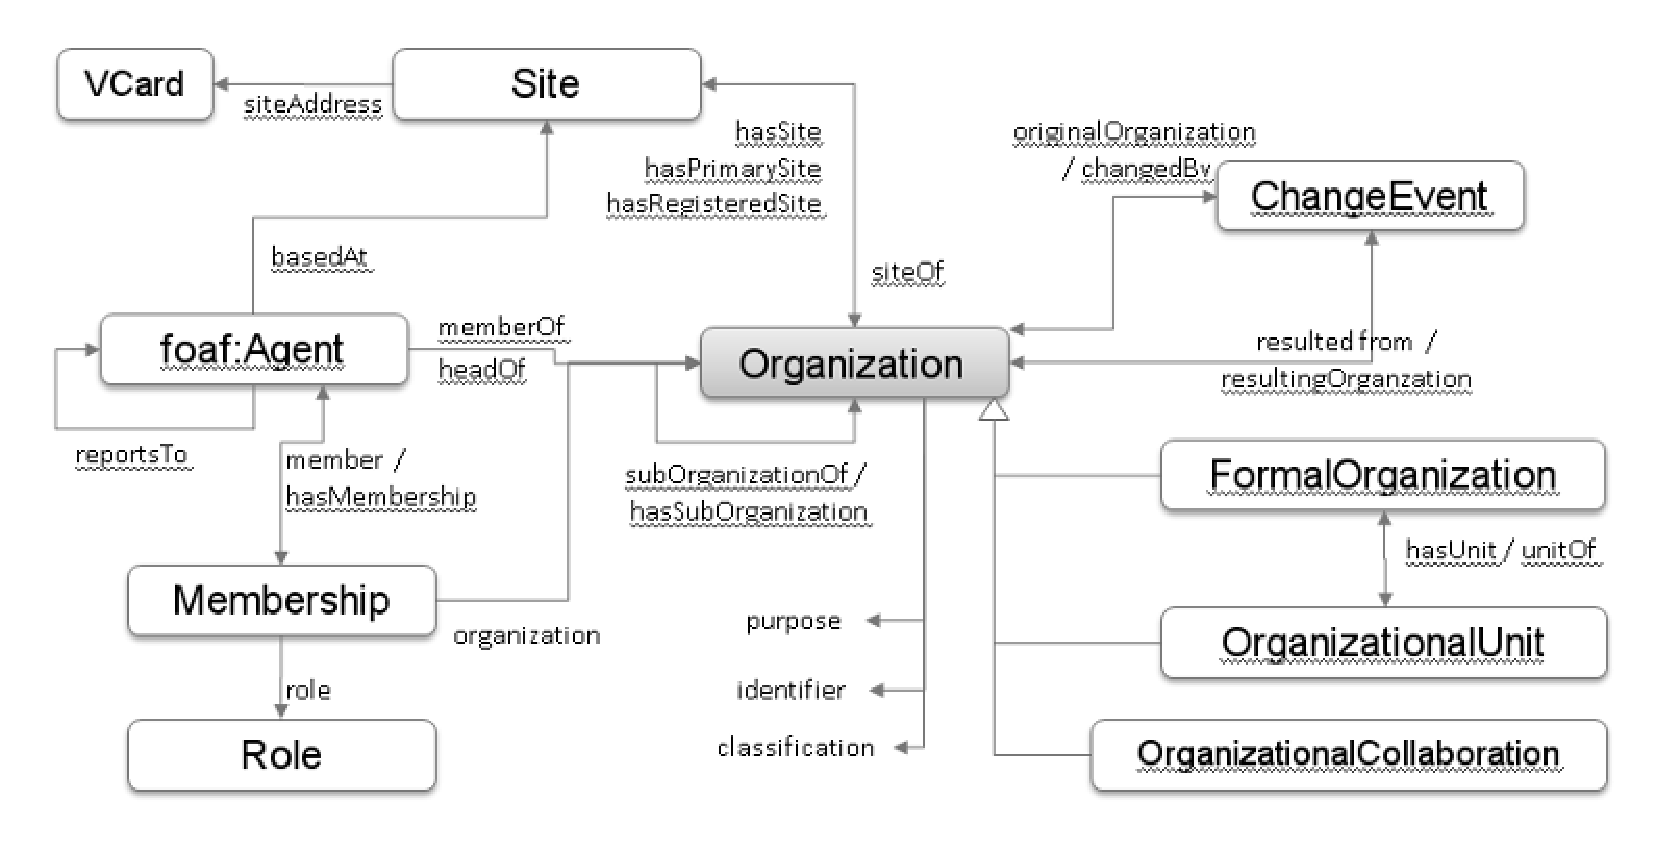
\includegraphics[width=14cm]{images/phd/org}
  \caption{\textit{Organizations Ontology. Overview.}}
 \label{fig:org-ontology}
\end{figure}

Desde otro punto de vista no tan centrado en la corriente de Web Semántica y ontologías, hay que referenciar 
la propuesta de datos abiertos realizada por \textit{OpenCorporates} a través ``\textit{The Open Database Of The Corporate World}'', han utilizado
técnicas de \textit{screen scrapping} y \textit{crawling} para extraer información de más de $12$ millones de compañías. Esta
información, ver Figura~\ref{figure:open-org}, tiene un alto valor para reutilizar y trazar la actividad de una empresa ya que disponen en la mayoría
de los casos del identificador de la empresa. La información de esta base de datos sigue un enfoque mixto entre \opendata y \linkeddata, 
pero el gran problema reside en la ausencia de un modelo formal para la descripción de los datos, es por ello que disponer de un modelo formal 
que integre esta información es clave para la posible reutilización de la información y explotación de la misma de una forma estándar.

\begin{figure}[!h]
\begin{center}
\begin{lstlisting}[language=SPARQL]
    <http://opencorporates.com/companies/nl/37136346.rdf?id=5828504>    
      a <http://purl.org/dc/dcmitype/Text>,
                foaf:Document;
         dct:format "application/rdf+xml";
         dct:isFormatOf 
	  <http://opencorporates.com/companies/nl/37136346?id=5828504>;
         dct:title "Linked Data in RDF format for Benuma";
         foaf:primaryTopic 
	  <http://opencorporates.com/id/companies/nl/37136346> .
	  ...
        <http://opencorporates.com/id/companies/nl/37136346>     
	a <http://s.opencalais.com/1/type/er/Company>;
         :label "Benuma" 
\end{lstlisting}
\caption{Información (parcial) sobre una Organización de ``Open Corporates'' en N3.}
\label{figure:open-org}
\end{center}
\end{figure}

\cleardoublepage
\subsubsection{Proyectos de Investigación}
Los proyectos de investigación de los principales programas competitivos
también se han visto involucrados en el despliegue de sistemas de contratación
pública electrónica utilizando semántica y datos enlazados. Entre ellos
se pueden destacar los siguientes:
\begin{description}
 \item [\textit{LOTED Project}~\cite{loted-project}] \textit{Linked Open Tenders Electronic Daily} realizado
por el grupo KMI de la \textit{Open University} del Reino Unido permite la consulta en \gls{SPARQL} de anuncios de licitación
publicados a través de los \gls{RSS} de \gls{TED}. Se trata del tradicional enfoque de \textit{Rdfizar}, información
ya publicada y hacerla disponible a través de un \textit{endpoint} de SPARQL. Sin duda se trata
de una importante iniciativa tanto por su carácter innovador, como por tratarse de la primera apuesta
real de utilización de semántica en los anuncios de licitación, sin embargo, tan sólo llega a los anuncios
de licitación publicados en TED y también parece que el demostrador oficial ha dejado de ser 
mantenido por los autores. No obstante, es necesario considerar esta propuesta para aprovechar
el efecto experiencia de la misma.
 \item [\textit{LOD2 Project}~\cite{lod2-project}.] Este proyecto europeo al que se ha referenciado en la
Sección~\ref{lod2-project} por su esfuerzo en la iniciativa \linkeddata desde un punto de vista genérico, también ha seleccionado la contratación pública electrónica como un caso de uso estratégico, es por ello
que han aumentado los paquetes de trabajo para incluir el esfuerzo de la \textit{Charles University} de la República Checa y su investigación sobre la aplicación de \linkeddata y semántica en el campo
del \eproc. Esto se ha manifestado en la constitución del paquete de trabajo \textit{WP9A – LOD2 for a Distributed Marketplace for Public Sector Contracts}.
La importancia del seguimiento de este proyecto reside tanto en las personas como en las instituciones implicadas, ya que generan 
una gran cantidad de tecnología y \textit{know-how} especialmente relevante para el estudio objeto de este documento y para las iniciativas
de \linkeddata y \opendata en general.
 \item [\textit{LATC Project}~\cite{latc-project}.] \textit{Linked open data around-the-clock} es un proyecto europeo,
una \textit{Specific Support Action} en el contexto del 7º Programa Marco-ICT formado por más de 58 instituciones
en los que se realizan y coordinan proyectos, personas. etc. El objetivo de este proyecto es gestionar la información
y datos generados a través de distintas fuentes proveyendo la infraestructura y documentación necesaria para
desplegar arquitecturas que den soporte a los datos enlazados. Prueba de su ingente capacidad es la cobertura y 
asesoramiento a proyectos y a investigadores de Europa (74\%) y de Estados Unidos (25\%). El consorcio
está formado por instituciones y empresas tan relevantes en este campo como: \textit{Digital Enterprise Research Institute} (DERI), \textit{NUI Galway}, Irlanda;
\textit{Vrije Universiteit Amsterdam} (VUA), Países Bajos; \textit{Freie Universit\"{a}t Berlin} (FUB), Alemania; \textit{Institute for Applied Informatics} e.V. (InfAI), Alemania y
\textit{Talis Information Ltd.}, Reino Unido.

\item [\textit{PlanetData Project}~\cite{planet-data-project}.] Se trata de una Red de Excelencia en el 
ámbito europeo (FP7-257641) con un presupuesto total de $3.72$ millones de euros y en la que participan los principales 
organismos de investigación con el objetivo de sumar los esfuerzos de la comunidad de investigadores para ofrecer 
a las organizaciones interesadas en la iniciativa de \linkeddata soporte con la publicación de sus datos. Evidentemente 
cuentan con un estrecho lazo con los proyectos anteriores y su actividad cubre las cuestiones relacionadas con datos enlazados 
en diferentes ámbitos: \textit{data streams, (micro) blog posts, digital archives, eScience resources, public sector data sets, and the Linked Open Data Cloud}.

\item [\textit{WebDataCommons.org}~\cite{web-data-commons-project}.] Es una iniciativa conjunta realizada por el grupo 
de investigación \textit{Web-based Systems Group} en la \textit{Freie Universit\"{a}t} de Berlín y el 
\textit{Institute AIFB} perteneciente al \textit{Karlsruhe Institute of Technology}, en el cual se han extraído 
y generado tripletas \gls{RDF} de más de $65$ millones de sitios web, contando un número de 
\textit{$3.2$ billion RDF quads} a fecha de febrero del año 2012, cubriendo información sobre productos, 
personas, organizaciones, lugares, eventos y recetas de cocina entre otros. Para la realización de este 
experimento se han utilizando técnicas de extracción de información de \gls{HTML} que utilizan microformatos, RDFa, etc. 
Toda esta información y datos está disponible para su descarga y uso por terceros en RDF. La importancia de este proyecto 
reside tanto en las personas y organizaciones implicadas como en la magnitud de los datos que han conseguido extraer.

\item [Otros proyectos.] Estas iniciativas trabajan con tecnología semántica y de datos enlazados en diferentes contextos suministrando servicios
a instituciones públicas o bien realizando investigación e innovación. Entre otros, se pueden citar: \gls{FP7} project SEALS (\textit{Semantic Evaluation at Large Scale}), FP7 project SpitFIRE (\textit{Semantic-Service Provisioning for the Internet of Things using Future Internet Research 
by Experimentation}), French DataLift project y Semic.EU.
\end{description}

Igualmente a nivel nacional se han impulsado diferentes iniciativas
y proyectos, como los de la República Checa y ``10ders Information Services'', que intentan elevar el significado de la información
de los anuncios de licitación utilizando tecnologías semánticas. También hay que considerar que la reutilización
de vocabularios ya establecidos e impulsados por las distintas Administración Públicas, por ejemplo la iniciativa Joinup~\cite{joinup-europe} de la Unión Europea, 
es de suma relevancia para proporcionar información utilizando datos enlazados, en este sentido todas las iniciativas y proyectos reseñados en las secciones anteriores ayudan a 
disponer de los \textit{building blocks} necesarios para afrontar la aplicación de semántica a los procesos de contratación pública electrónica.

% 10-15


\printindex
\printglossaries


% Bibliografía
\insertbibliography
\end{document}
